\documentclass[
    bachelor,
    % bigskip, % sets linespread factor to 1.5
    % nofont, % remember to manally set the fonts
    truefont,
    % sourcefont,
    pdflinks,
    %colorlinks,
    %compact,
]{xjtuthesis}

\graphicspath{{figures/}}

\usepackage{tikz}
\usepackage{etoolbox}
\usetikzlibrary{shapes.arrows}
\definecolor{redtop}{HTML}{ffebee}
\definecolor{redfront}{HTML}{ffebee}
\definecolor{redright}{HTML}{ffcdd2}
\definecolor{redline}{HTML}{ef9a9a}

\definecolor{bluetop}{HTML}{e0f7fa}
\definecolor{bluefront}{HTML}{e0f7fa}
\definecolor{blueright}{HTML}{b2ebf2}
\definecolor{blueline}{HTML}{80deea}

\definecolor{greentop}{HTML}{e8f5e9}
\definecolor{greenfront}{HTML}{e8f5e9}
\definecolor{greenright}{HTML}{c8e6c9}
\definecolor{greenline}{HTML}{a5d6a7}

\definecolor{yellowtop}{HTML}{fff176}
\definecolor{yellowfront}{HTML}{fff176}
\definecolor{yellowright}{HTML}{ffee58}
\definecolor{yellowline}{HTML}{ffeb3b}

\definecolor{orangetop}{HTML}{fffde7}
\definecolor{orangefront}{HTML}{fff3e0}
\definecolor{orangeright}{HTML}{ffe0b2}
\definecolor{orangeline}{HTML}{ffcc80}

\definecolor{browntop}{HTML}{efebe9}
\definecolor{brownfront}{HTML}{efebe9}
\definecolor{brownright}{HTML}{d7ccc8}
\definecolor{brownline}{HTML}{bcaaa4}

\definecolor{darkbluetop}{HTML}{f5f5f5}
\definecolor{darkbluefront}{HTML}{eeeeee}
\definecolor{darkblueright}{HTML}{e0e0e0}
\definecolor{darkblueline}{HTML}{bdbdbd}

\definecolor{purpletop}{HTML}{f3e5f5}
\definecolor{purplefront}{HTML}{f3e5f5}
\definecolor{purpleright}{HTML}{e1bee7}
\definecolor{purpleline}{HTML}{ce93d8}

\newcommand\cube[7]{
    \ifstrequal{#7}{blue}{
        \def\top{bluetop}
        \def\front{bluefront}
        \def\right{blueright}
        \def\line{blueline}
    }{\ifstrequal{#7}{red}{
        \def\top{redtop}
        \def\front{redfront}
        \def\right{redright}
        \def\line{redline}
    }{\ifstrequal{#7}{yellow}{
        \def\top{yellowtop}
        \def\front{yellowfront}
        \def\right{yellowright}
        \def\line{yellowline}
    }{\ifstrequal{#7}{orange}{
        \def\top{orangetop}
        \def\front{orangefront}
        \def\right{orangeright}
        \def\line{orangeline}
    }{\ifstrequal{#7}{green}{
        \def\top{greentop}
        \def\front{greenfront}
        \def\right{greenright}
        \def\line{greenline}
    }{\ifstrequal{#7}{brown}{
        \def\top{browntop}
        \def\front{brownfront}
        \def\right{brownright}
        \def\line{brownline}
    }{\ifstrequal{#7}{darkblue}{
        \def\top{darkbluetop}
        \def\front{darkbluefront}
        \def\right{darkblueright}
        \def\line{darkblueline}
    }{\ifstrequal{#7}{purple}{
        \def\top{purpletop}
        \def\front{purplefront}
        \def\right{purpleright}
        \def\line{purpleline}
    }{
        \def\top{bluetop}
        \def\front{bluefront}
        \def\right{blueright}
        \def\line{blueline}
    }}}}}}}}
    \fill[fill=\front,draw=\line,shift={(0,0,0)}](#1,#2,#3)--(#1+#4,#2,#3)--(#1+#4,#2+#5,#3)--(#1,#2+#5,#3)--cycle;
    \fill[fill=\top,draw=\line,shift={(0,#5,0)}](#1,#2,#3)--(#1+#4,#2,#3)--(#1+#4,#2,#3-#6)--(#1,#2,#3-#6)--cycle;
    \fill[fill=\right,draw=\line,shift={(#4,0,0)}](#1,#2,#3)--(#1,#2,#3-#6)--(#1,#2+#5,#3-#6)--(#1,#2+#5,#3)--cycle;
}

\newcommand\featuremap[1]{
    \cube{0}{0}{0}{8}{24}{6}{#1}
    \foreach \x in {0, ..., 7} {
        \foreach \y in {0, ..., 23} {
            \cube{\x}{\y}{0}{1}{1}{1}{#1}
        }
    }
}

\newcommand\pcb{
    \foreach \x in {0, ..., 7} {
        \foreach \y in {0, ..., 3} {
            \cube{\x}{\y+0}{0}{1}{1}{6}{blue}
            \cube{\x}{\y+0}{0}{1}{1}{1}{blue}
        }
    }
    \foreach \x in {0, ..., 7} {
        \foreach \y in {0, ..., 3} {
            \cube{\x}{\y+4}{0}{1}{1}{6}{red}
            \cube{\x}{\y+4}{0}{1}{1}{1}{red}
        }
    }
    \foreach \x in {0, ..., 7} {
        \foreach \y in {0, ..., 3} {
            \cube{\x}{\y+8}{0}{1}{1}{6}{purple}
            \cube{\x}{\y+8}{0}{1}{1}{1}{purple}
        }
    }
    \foreach \x in {0, ..., 7} {
        \foreach \y in {0, ..., 3} {
            \cube{\x}{\y+12}{0}{1}{1}{6}{green}
            \cube{\x}{\y+12}{0}{1}{1}{1}{green}
        }
    }
    \foreach \x in {0, ..., 7} {
        \foreach \y in {0, ..., 3} {
            \cube{\x}{\y+16}{0}{1}{1}{6}{brown}
            \cube{\x}{\y+16}{0}{1}{1}{1}{brown}
        }
    }
    \foreach \x in {0, ..., 7} {
        \foreach \y in {0, ..., 3} {
            \cube{\x}{\y+20}{0}{1}{1}{6}{orange}
            \cube{\x}{\y+20}{0}{1}{1}{1}{orange}
        }
    }
    \foreach \y in {0, ..., 5} {
        \draw[draw=black, line width=0.06em, shift={(0, 4*\y, 0)}] (0,0) -- (8,0) -- (8,4) -- (0,4) -- cycle;
    }
}

\newcommand\colvector{
    \cube{0}{1.5+0 }{0}{1}{1}{6}{blue}
    \cube{0}{1.5+4 }{0}{1}{1}{6}{red}
    \cube{0}{1.5+8 }{0}{1}{1}{6}{purple}
    \cube{0}{1.5+12}{0}{1}{1}{6}{green}
    \cube{0}{1.5+16}{0}{1}{1}{6}{brown}
    \cube{0}{1.5+20}{0}{1}{1}{6}{orange}
    \foreach \y in {0, ..., 5} {
        \draw[draw=black, line width=0.06em, shift={(0, 1.5+4*\y, 0)}] (0,0) -- (1,0) -- (1,1) -- (0,1) -- cycle;
    }
}

\newcommand\classify[3]{
    \draw[draw=#3,line width=0.15em,rounded corners=0.4em] (#1-3,#2-3) rectangle (#1+21,#2+3);
    \draw[line width=0.15em] (#1+0,#2+0) circle[radius=2];
    \draw[line width=0.15em] (#1+6,#2+0) circle[radius=2];
    \draw[font=\fontsize{20em}{6}\selectfont] node at (#1+12,#2+0) {...};
    \draw[line width=0.15em] (#1+18,#2+0) circle[radius=2];
}

\newcommand\softmax{
    \classify{0}{0}{blueline}
    \classify{0}{8}{redline}
    \classify{0}{16}{purpleline}
    \classify{0}{24}{greenline}
    \classify{0}{32}{brownline}
    \classify{0}{40}{orangeline}
}

\newcommand\notes[3]{
    \node[draw, single arrow,
          minimum height=11em, minimum width=8em,
          single arrow head extend=0.5em,
          anchor=west] at (#1,#2) {};
    \node[font=\fontsize{5em}{6}\selectfont] at (#1+1.5, #2+3) {#3};
}

\tikzset{global scale/.style={
    scale=#1,
    every node/.append style={scale=#1}
}}

\newcommand\figarchpcb{
    \begin{tikzpicture}[line join=round, line width=0.05em, global scale=0.18]
        \begin{scope}[shift={(0,1.5,0)}]
            \node[anchor=south west]{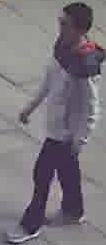
\includegraphics[width=26em]{person}};
        \end{scope}
        \begin{scope}[shift={(20,0,0)}]
            \featuremap{darkblue}
        \end{scope}
        \begin{scope}[shift={(40,0,0)}]
            \pcb
        \end{scope}
        \begin{scope}[shift={(60,0,0)}]
            \colvector
        \end{scope}
        \begin{scope}[shift={(75,3,0)},global scale=0.5]
            \softmax
        \end{scope}
        \notes{13}{12}{ResNet50}
        \notes{33}{12}{均匀分块}
        \notes{53}{12}{区域池化}
        \notes{66.5}{23}{}
        \notes{66.5}{19}{}
        \notes{66.5}{15}{}
        \notes{66.5}{11}{}
        \notes{66.5}{7}{}
        \notes{66.5}{3}{}
        \node[font=\fontsize{5em}{6}\selectfont] at (68, 26) {分类};
    \end{tikzpicture}
}

\usepackage{wrapfig} % 多张图片
\usepackage{overpic} % mask_rcnn
\usepackage{algorithm} % 算法框图
\usepackage{algorithmicx}
\usepackage{algpseudocode}
\floatname{algorithm}{算法}
\renewcommand{\algorithmicrequire}{\textbf{输入:}}
\renewcommand{\algorithmicensure}{\textbf{输出:}}

% \let\cite=\supercite

% 将引用的文献的 BibTeX 放入 bibliography.bib
\addbibresource{bibliography.bib}

\begin{document}

    % 主要信息
    % 标题,中文
\ctitle{面向多CPU集群的深度行人重识别研究}
\covertitlefirst{面向多CPU集群的}
\covertitlesecond{深度行人重识别研究}
\cschool{电信}
\cactualinstitution{电信学院}
\cmajor{计算机科学与技术}
\cclass{计算机44}
\cyear{\the\year}
\cmonth{\the\month}

% 作者,中文
\cauthor{李源勋}
\stuid{2140505083}

% 学科,中文,本科生不需要
\csubject{}

% 导师姓名,中文
\csupervisor{何\quad 晖}

% 关键词,中文。用全角分号「;」分割
% 研究生的应首先从《汉语主题词表》中摘选
\ckeywords{行人重识别;深度学习;强化学习;多CPU集群}

% 提交日期,本科生不需要
\cproddate{\the\year 年\the\month 月}

% 论文类型,中文,本科生不需要
% 从理论研究、应用基础、应用研究、研究报告、软件开发、设计报告、案例分析、调研报告、其它中选择
\ctype{}

% 论文标题,英文
\etitle{Research for Multi-CPU Cluster Based Person Re-Identification}

% 作者姓名,英文
\eauthor{Yuanxun Li}

% 学科,英文,本科生不需要
\esubject{}

% 导师姓名,英文
\esupervisor{Hui He}

% 关键词,英文。用半角分号和一个半角空格「; 」分割
\ekeywords{Person Re-Identification; Deep Learning; Reinforcement Learning; Multi-CPU Cluster}

% 学科门类,英文
% 从Philosophy(哲学)、Economics(经济学)、Law(法学)、Education(教育学)、Arts(文学)、
%   Science(理学)、Engineering Science(工学)、Medicine(医学)、Management Science(管理学)中选择
\ecate{Engineering Science}

% 提交日期,英文,本科生不需要
% 应当和 cproddate 保持一致
\eproddate{\monthname{\month}\ \the\year}

% 论文类型,英文,本科生不需要
% 从Theoretical Research(理论研究)、Application Fundamentals(应用基础)、Applied Research(应用研究)、
%   Research Report(研究报告)、Software Development(软件开发)、Design Report(设计报告)、
%   Case Study(案例分析)、Investigation Report(调研报告)、其它(Other)中选择
\etype{}

% 摘要,中文。段间空行
\cabstract{
    随着视频监控技术的发展,无人值守的视频监控设备被越来越普遍地部署在国民社会的各个方面,在公安、交通、智能楼宇、金融、司法、教文卫等领域都有着不可替代的作用。具体的应用场景包括平安城市、卡口系统、工地监控、自助银行、监狱劳教和学前教育等。

    在视频监控领域一个很重要且极具挑战性的问题是行人的重识别。行人重识别,指的是在多个视野不重叠的监控视频中,重新识别那些之前出现过的行人,即把当前行人与之前已标记的人物相对应。该工作的实现可以为人物搜索、特定人物跟踪等应用提供强有力的支持,进而应用在平安城市、工地监控、学前教育等场景。

    要实现行人的重识别需要借助计算机视觉领域的技术。目前的计算机视觉算法的前沿关注点主要集中在深度学习技术。由于深度学习的海量计算需求和GPU强大的并行计算能力,大部分深度学习算法都是借助GPU来调整模型参数。然而目前的GPU的RAM十分有限,这就约束了深度神经网络的深度和训练速度,限制了其对于很多具体问题,包括行人重识别问题,的研究空间和具体应用。

    超级计算机是计算机中功能最强、运算速度最快、存储容量最大的一类计算机,多用于国家高科技领域和尖端技术研究,是一个国家科研实力的体现,它对国家安全,经济和社会发展具有举足轻重的意义。目前由于成本问题,基于超算的深度学习架构还不够流行,这既限制了科研理论的发展,又没有使超算发挥其应有的作用。

    因此,本项目将探索在多CPU集群上的深度行人重识别问题,致力于在项目过程中发现和解决问题,推动理论的发展和实际的应用。
}

% 摘要,英文。段间空行
\eabstract{
    With the development of video surveillance technology, unattended video surveillance devices are being deployed more and more widely in various aspects of the civil society, and are irreplaceable in fields such as public security, transportation, intelligent buildings, finance, justice, and education. The role. Specific application scenarios include Pingan City, bayonet system, site monitoring, self-service banking, prison labor camps and pre-school education.

    A very important and challenging issue in video surveillance is pedestrian recognition. Pedestrian re-identification refers to the re-identification of pedestrians who have previously appeared in multiple surveillance videos that do not overlap, that is, to associate the current pedestrian with the previously marked person. The implementation of this work can provide strong support for applications such as character search and specific person tracking, and it can be used in scenes such as safe city, site monitoring, and preschool education.

    To achieve pedestrian re-identification requires the use of computer vision technology. The frontier focus of current computer vision algorithms is mainly on deep learning techniques. Due to the massive computing requirements of deep learning and the GPU's powerful parallel computing capabilities, most of the deep learning algorithms use GPUs to adjust model parameters. However, the current GPU has very limited RAM, which limits the depth and training speed of deep neural networks, and limits its research space and specific applications for many specific issues, including pedestrian re-identification issues.

    The supercomputer is a type of computer with the most powerful functions, the fastest computing speed, and the largest storage capacity. It is mostly used in the research of high-tech fields and cutting-edge technologies of the country. It is a manifestation of the strength of scientific research in a country. It is a national security, economic and social development. Has a significant significance. At present, because of the cost problem, the deep learning framework based on super-calculation is not yet popular enough. This not only limits the development of scientific research theory, but also does not make super-calculation play its due role.

    Therefore, this project will explore in-depth pedestrian re-identification issues on multi-CPU clusters, commit to discovering and resolving problems during the project process, and promote theoretical development and practical application.
}

    % 任务书信息
    \taskmajor{计算机科学与技术}
\taskpresident{唐亚哲}
\taskapprovaldate{2018-03-05}
\taskschool{电子与信息工程}
\taskclass{计算机~44}
\taskauthor{李源勋}
\tasktitle{面向多CPU集群的深度行人重识别研究}
\taskfromyear{2018}
\taskfrommonth{2}
\taskfromday{26}
\tasktoyear{2018}
\tasktomonth{6}
\tasktoday{1}
\taskplace{西安交通大学}

\taskbackground{
    \uline{随着视频监控技术的发展,无人值守的视频监控设备被越来越普遍地部署在国民社会的各个方面,在公安、交通、智能楼宇、金融、司法、教文卫等领域都有着不可替代的作用。具体的应用场景包括平安城市、卡口系统、工地监控、自助银行、监狱劳教和学前教育等。}

    \uline{在视频监控领域一个很重要且极具挑战性的问题是行人的重识别。行人重识别,指的是在多个视野不重叠的监控视频中,重新识别那些之前出现过的行人,即把当前行人与之前已标记的人物相对应。在此基础上,对于现实场景中监控设备的部署位置,也是一个非常值得研究的问题,该工作的实现可以为监控设备的部署位置提供参考,为人物搜索、特定人物跟踪等应用提供更加准确、高效的性能,进而应用在平安城市、工地监控、学前教育等场景。}

    \uline{要实现行人的重识别需要借助计算机视觉领域的技术。目前的计算机视觉算法的前沿关注点主要集中在深度学习技术。由于深度学习的海量计算需求和GPU强大的并行计算能力,大部分深度学习算法都是借助GPU来调整模型参数。然而目前的GPU的RAM十分有限,这就约束了深度神经网络的深度和训练速度,限制了其对于很多具体问题,包括行人重识别问题,的研究空间和具体应用。}

    \uline{超级计算机是计算机中功能最强、运算速度最快、存储容量最大的一类计算机,多用于国家高科技领域和尖端技术研究,是一个国家科研实力的体现,它对国家安全,经济和社会发展具有举足轻重的意义。目前由于成本问题,基于超算的深度学习架构还不够流行,这既限制了科研理论的发展,又没有使超算发挥其应有的作用。}

    \uline{因此,本项目将探索在多CPU集群上的深度行人重识别问题,致力于在项目过程中发现和解决问题,推动理论的发展和实际的应用。}
}

\taskrawmaterial{
    \uline{在行人重识别领域公认的用于评定一个模型效果的数据集有:VIPeR~\mbox{\cite{gray2007evaluating}}、CUHK01~\mbox{\cite{li2012human}}、CUHK03~\mbox{\cite{li2012human}}、Market-1501~\mbox{\cite{zheng2015scalable}}、DukeMTMC-reID~\mbox{\cite{ristani2016MTMC}}。}

    \uline{毕业设计的资料包括国际上前沿的计算机视觉领域,特别是有关行人重识别问题的期刊、会议论文。~\mbox{\cite{ren2015faster,li2014deepreid,ristani2016MTMC,sun2017beyond,he2017mask,he2016deep,chen2018person}}}
}

\taskmaintask{
    \begin{enumerate}
        \item \uline{将目前的深度行人重识别工程改造为适用于多CPU集群的形式。}
        \item \uline{将工程部署在天河二号集群中,解决过程中遇到的具体问题。}
        \item \uline{采集同一地点不同视角的摄像头监控录像,作为实验数据。}
        \item \uline{研究摄像头的部署位置对于行人重识别算法性能的影响,求解最优部署方案。}
        \item \uline{对工程进行速度和正确率方面的性能优化。}
        \item \uline{总结经验和结论。}
    \end{enumerate}
}

\taskrequirement{
    \begin{enumerate}
        \item \uline{能够将现有的行人重识别算法运行在多CPU集群上。}
        \item \uline{采集的监控录像符合实验要求。}
        \item \uline{对于摄像头部署位置的研究能够得出合理的实验结果。}
        \item \uline{对于实验结果得出合理的经验和结论。}
    \end{enumerate}
}

\taskfinalmaterial{
    \uline{毕业设计论文不少于 15000 字,英文文献翻译不少于 5000 字。}
}

\taskothertaskreference{
}
    % 评审意见信息
    \reviewschool{电子与信息工程}
\reviewmajor{计算机科学与技术}
\reviewclass{计算机44}
\reviewauthor{李源勋}
\reviewtitle{面向多CPU集群的深度行人重识别研究}
\reviewteachercomment{
    论文针对无人值守的视频监控,实现了行人重识别领域最新的研究成果,同时推出了一个全新的、包含多个摄像头的数据集的初始版本,提出了基于强化学习的摄像头部署方案选择模型。论文还展示了将模型部署在多CPU 集群上训练的结果,研究了多CPU 集群对于深度神经网络的训练过程的影响。论文工作难度较大,工作量饱满。\\
    该生在毕业设计工作中学习态度积极主动,工作认真努力。从论文完成情况看,该生掌握了扎实的专业基础理论和专业知识,具有较强的独立工作能力。论文达到了工学学士学位要求。专业英语文献翻译良好。
    }
\reviewteachergrade{优秀}
\reviewteachername{何晖}
\reviewteacheryear{2018}
\reviewteachermonth{6}
\reviewteacherday{11}

\reviewercomment{}
\reviewergrade{}
\reviewername{侯迪}
\reviewertitle{副教授}
\revieweryear{2018}
\reviewermonth{6}
\reviewerday{11}

\resultschool{电子与信息工程学}
\resultmajor{计算机科学与技术}
\resultauthor{李源勋}
\resulttitle{面向多CPU集群的深度行人重识别研究}
\resultcomment{}
\resultgrade{}
\resultprincipal{}
\resultmenberaname{}
\resultmenberatitle{}
\resultmenberbname{}
\resultmenberbtitle{}
\resultmenbercname{}
\resultmenberctitle{}
\resultyear{2018}
\resultmonth{6}
\resultday{11}

    % 封面
    \xjtuchead
    % 任务书
    \ctaskdescription
    % 评审意见
    \creviewopinion
    % 答辩结果
    \cfinalresult
    % 中文摘要
    \xjtucinfopage
    % 英文摘要
    \xjtueinfopage
    % 目录
    \xjtutoc

    % 主要符号表,可以没有
    \begin{denotation}
    \item[$A$]              智能体所能采取的行动的集合
    \item[$\mathcal{D}^{src}$]    行人重识别源数据集
    \item[$\mathcal{D}^{src}$]    行人重识别目标数据集
    \item[$\mathcal{E}$]    模型效果评估指标
    \item[$\mathcal{F}$]    行人重识别模型
    \item[$\mathcal{I}$]    视频画面帧集合
    \item[$P$]              智能体采取行动的策略
    \item[$r$]              智能体从环境中得到的反馈
    \item[$S$]              摄像头方案(当前状态)集合
    \item[$V$]              当前状态的长期价值
    \item[$\alpha$]         智能体的参数学习率
    \item[$\gamma$]         智能体的远见性
    \item[$\pi$]            状态转移概率
\end{denotation}


    % 正文
    \xjtucontent
    \newrefsection
        % 绪论
        \chapter{绪论}\label{sec:introduction}

本章首先阐述了论文的研究背景,说明论文的动机和主要观点。接着介绍了与论文主题密切相关的前人工作,分析评价其贡献与不足。然后形式化地对要解决的问题进行定义,明确研究工作的界限和规模。最后介绍论文的主要工作,以及论文的组织结构。

\section{研究背景}

随着视频监控技术的发展,无人值守的视频监控设备被越来越普遍地部署在国民社会的各个方面,在公安、交通、智能楼宇、金融、司法、教文卫等领域都有着不可替代的作用。具体的应用场景包括平安城市、卡口系统、工地监控、自助银行、监狱劳教和学前教育等。

在视频监控领域一个很重要且极具挑战性的问题是行人的重识别。行人重识别,指的是对多个视野不重叠的监控摄像头拍摄的同一个行人的图片进行匹配\cite{chen2018person},即重新识别一些之前出现过的行人。该工作的实现可以为人物搜索、特定人物跟踪等应用提供强有力的支持,进而应用在平安城市、工地监控、学前教育等场景。

行人重识别技术在实际应用中受诸多因素的影响,包括摄像头的部署位置、成像质量以及摄像头数量等等。面对一个从未部署过摄像头的监控场景,一个优秀的摄像头位置部署方案可以实现监控范围无死角、行人重识别准确率高以及跨摄像头持续跟踪的连续性强的效果。影响摄像头成像质量的因素有很多,包括摄像头自身的性能参数,摄像头部署角度不同导致的不同视野范围,以及摄像头的部署位置不同导致的不同光线条件。在理想情况下,摄像头的数量越多,得到的行人信息就越多,更有利于行人重识别算法的实施。但是在预算有限的情况下,摄像头的数量不可能无限增加。因此,如何选择摄像头的数量及其部署位置,使得行人重识别算法的性能最大化,便成为一个极具现实意义的研究问题。

要实现行人的重识别需要借助计算机视觉领域的技术。目前的计算机视觉算法的前沿关注点主要集中在深度学习技术。由于深度学习的海量计算需求和GPU强大的并行计算能力,大部分深度学习模型都是借助GPU来调整模型参数。然而使用GPU进行运算也存在许多问题,例如GPU设备通常比较昂贵,且少见于嵌入式设备中。同时GPU的显存普遍不高,限制了模型的规模以及每一批次数据的规模。与此同时,多CPU集群具有硬件成本低、搭建方式灵活以及部署广泛等优点,然而对于深度学习算法在多CPU集群上的研究与应用少之又少。因此,有必要对深度学习算法在多CPU集群上的性能表现进行深入的调查、分析和研究。

\section{研究现状}
本节介绍了与本课题密切相关的三个领域,行人重识别、多摄像头选择以及多CPU集群,其中的前人工作以及研究现状。

\subsection{行人重识别}

行人重识别的任务是将多个视野不重叠的监控摄像头所拍摄的同一行人进行匹配\cite{chen2018person}。与用于身份认证的人脸识别技术不同的是,行人重识别技术不是针对某个特定的行人进行建模,因为测试环节的数据可能没有在训练环节出现过。因此,行人重识别模型需要学习到一种判别两张图片空间特征和语义特征相似度的能力。要拥有该能力,则需要行人重识别模型具有强大的特征提取功能和距离度量功能。一个优秀的特征提取模型能够将行人图片中最具有判别性的特征很好地提取和表示,使得在所构造的特征空间内,不同行人所对应的特征的分界面尽可能地宽阔。一个优秀的距离度量模型能够使得相同行人的特征之间的距离尽可能近,不同行人的特征之间的距离尽可能远,即在特征空间内能够很好的将行人的特征进行正确地聚类。基于这样两个通用的建模阶段,在行人重识别领域研究的方法也主要分为两大类:基于表征学习(Representation Learning)的方法和基于度量学习(Metric Learning)的方法。

基于表征学习的方法将主要精力用于使模型拥有强有力的特征表示能力,使模型能够发现并表示行人图片中具有判别性的空间特征(如肤色、头发、衣着等)和语义特征(如性别、姿态、行为等)。得益于近年来深度学习\cite{simonyan2014very},尤其是深度卷积神经网络\cite{krizhevsky2012imagenet}(Convolutional Neural Network, CNN)的发展,现有的CNN已经能很好地抽取图片中的空间特征和语义特征,并将其用于特定的学习任务。因此,当前的基于表征学习的方法越来越多地将目光转向了基于CNN的特征表示。基于表征学习的方法所表示的特征根据其表达所涵盖的范围,又可分为全局特征和局部特征。全局特征指的是将整张图片看作一个整体,模型一次性地将图片的特征表示出来,最终生成的特征表示虽然也有可能会有图片局部的特征,但该局部的位置不是固定的,并不能稳定、有效地表达人体各个部位有别于其他行人的特征。与此相反,局部特征是将行人图像划分切块后,对于每个局部进行特征提取,划分的方式可以是简单的均匀划分\cite{sun2017beyond},也可以是不均匀的(例如根据人体姿势骨架关键点\cite{zheng2017pose})划分。在Sun等人\cite{sun2017beyond}的工作中,既实现了一个基于均匀分块的强有力的基线模型(baseline model),使用非常简单、直观的方法取得了非常稳定、出色的效果;又提出了一种将行人图片中不同的像素块分类到行人不同部分的方法,使得行人的特征表示在基线模型的基础上更加稳健,该模型是行人重识别领域中的最新成果(state-of-the-art)。

基于度量学习的方法致力于找到一种合理的度量方式,使得相同行人特征之间的距离尽可能近,不同行人特征之间的距离尽可能远。基于度量学习的方法主要分成两大类:注重可解释性的传统的字典学习方法,以及基于深度学习的损失方法。字典学习方法将原始行人图片的特征向量映射到一个新的向量空间,在该向量空间中相同行人特征向量之间的距离普遍小于不同行人特征向量之间的距离。字典学习经常使用稀疏编码\cite{lee2007efficient}的思想实现。字典学习的训练过程通常会配合一个带有明确目的性的损失函数来实现,例如在Li等人\cite{li2018discriminative}的工作中通过半耦合的字典学习方法,设计了一个能够降低同一行人的不同分辨率图片之间的特征差异的损失函数,提升了行人重识别算法在不同分辨率下的识别效果。基于深度学习的损失方法主要将精力用于构造一个适合的损失函数,利用损失函数来引导深度神经网络的训练。常见的损失函数包括分类损失、三元组损失\cite{schroff2015facenet}、四元组损失\cite{chen2017beyond}以及边界挖掘损失\cite{xiao2017margin},这些损失函数大多受人脸识别领域研究的启发,为特定的研究目标针对性地设计损失函数,借助深度神经网络强大的学习能力,取得了优异的效果。

从当前的研究形势来看,基于度量学习的方法同样依赖一个强大的表征学习模型,才能从原始行人图片中提取到合适的特征表达。同时目前基于度量学习的方法也越来越多地使用深度神经网络来作为前端,也可以把前端看作是一个特征提取的过程。因此,深度神经网络这一工具将会越来越多地被用于行人重识别领域,同时也会促进表征学习和度量学习的融合。然而基于深度学习的行人重识别方法也存在一些问题,例如其训练和预测过程的计算量过于庞大,且高度依赖GPU,不适合部署在实时视频监控场景。

\subsection{多摄像头选择}

近年来,在行人重识别领域出现了一些多摄像头的数据集,如Zheng等人公开的Market1501\cite{zheng2015scalable}和Gou等人公开的DukeMTMC4ReID\cite{gou2017dukemtmc4reid}数据集,它们分别包含6个和8个摄像头。然而这些数据集的评估协议(Evaluation Protocol)与双摄像头的行人重识别数据集的评估协议一脉相承,最大的区别仅仅在于多摄像头评估协议会将排序结果中来自同一摄像头的同一行人图像排除。这样的评估方式没有很好地利用多个摄像头的信息,且与多摄像头在实际监控场景中的需求不符。例如在实际的监控场景中,往往要求多个摄像头所拍摄的同一行人图片都识别准确,才算这一个行人的识别结果正确,这样的要求大大提高行人重识别问题的难度和挑战性,也更符合实际应用。

多摄像头选择问题虽然在行人重识别领域尚欠研究,但是在目标追踪领域已有不少研究成果。在多摄像头目标追踪领域,多个摄像头会组成一个摄像头网络,各摄像头同步地拍摄视频画面,并与其它摄像头交换信息,以提升目标追踪的准确率。Bernab{\'e}等人\cite{de2012entropy}提出了基于信息熵的算法,该算法动态地选择一些摄像头,在一定的传输带宽限制、传输错误率限制以及运算量限制下,达到最优的准确率。如果选择某个摄像头所带来的准确率收益大于该摄像头产生的传输和运算量负担,那么就会选择该摄像头。Bhuvana等人\cite{bhuvana2016multi}提出了新颖度(surprisal)的概念,每个摄像头可以独立地计算其所拍摄的画面中的信息量,并且根据期望的摄像头数量,动态确定一个信息量阈值,只有当该摄像头画面中的信息量大于该阈值,才会选择该摄像头。在目标追踪领域的多摄像头选择研究也存在着一些不适用于行人重识别问题的情况和假设,例如在目标追踪问题中多个摄像头的视野都是重叠的,行人视频画面都是同步的,如此一来多个摄像头仅仅是同一行人、同一时刻的不同角度信息,不符合行人重识别领域中视野不重叠的要求。更进一步地,在同一时刻各摄像头只会拍到一个行人,所以摄像头之间不存在行人重识别的问题,只需要准确定位目标的位置。

要研究摄像头的数量与部署位置对行人重识别算法的影响,数据集需要满足以下要求:一、数据集中摄像头数量大于10,以便控制增减摄像头的进行分析对比,分析摄像头的拍摄位置对于监控效果的影响;二、存在视野重叠或拍摄位置接近的摄像头,以便分析同一位置、不同拍摄角度的拍摄方案对于监控效果的影响。三、行人需要出现在多个(而不仅仅是两个)摄像头画面内,且摄像头的分布呈路线状(可以存在分支),这样更符合行人跟踪的定义,更好地评估摄像头部署位置的监控效果。

目前主流的行人重识别数据库包括VIPeR\cite{gray2007evaluating}、CUHK01\cite{li2012human}、Market1501\cite{zheng2015scalable} 和 DukeMTMC4reID\cite{ristani2016MTMC},其摄像头数量分别为2、2、10、6和8个,由于摄像头的数量较少,不利于分析增减摄像头以评估摄像头数量对监控效果的影响。同时,包括 CUHK03\cite{li2014deepreid} 在内的所有数据集都缺乏单个行人持续追踪的场景,不利于实现监控效果的评估。

行人重识别领域的多摄像头选择问题是一个非常具有现实意义的问题,但由于以往数据库中摄像头个数的限制,以及现有的评估方式的不足,所以该问题至今还没有被深入地研究。因此,有必要针对上述需求重新采集一个数据库,满足研究和实验的需求。

\subsection{多CPU集群}

自上个世纪以来,半导体技术和制造工艺飞速发展,芯片制造成本大大降低,当前的半导体技术和制造工艺也越来越接近经典物理定律的极限,因此人们把目光由单核处理器转向了多核处理器,以及多CPU集群计算。在解决CPU集群中各节点通信问题时,主要采用两种方案:MPI\cite{sur2006high}和OpenMP\cite{dagum1998openmp}。其中MPI是一个消息传递接口,OpenMP是共享内存编程的工业标准。基于这些接口和标准,出现了很多运行在多CPU集群上的应用\cite{rabenseifner2009hybrid,ayguade2009design}。然而多CPU集群在深度学习方面的应用少之又少,其重要原因为GPU强大的并行计算能力。然而GPU计算也存在不足之处,如价格昂贵、配置复杂、显存不足等。这些问题正好是多CPU集群的优势。因此,分析、研究深度学习在多CPU集群上的性能表现是一件非常有意义的事情。

\section{研究问题}

本节对论文要解决的问题进行形式化表述。

给定源数据集$\mathcal{D}^{src}$,包含多标签、多摄像头、标注质量高的行人重识别数据集,用于行人重识别基线模型的训练。数据集$\mathcal{D}^{src}$需要包括训练集$\mathcal{D}_{train}^{src}$、测试查询集$\mathcal{D}_{query}^{src}$以及测试候选集$\mathcal{D}_{gallery}^{src}$。其中训练集$\mathcal{D}_{train}^{src}$为包含行人标签的图片集,方便用于训练阶段的标签分类任务。测试查询集$\mathcal{D}_{query}^{src}$包含多张标注有标签和摄像头的ground truth的图片,在模型评估阶段,将每张图片$\mathcal{D}_{query,\,(i)}^{src}$输入模型,模型从测试候选集$\mathcal{D}_{gallery}^{src}$中抽取出与$\mathcal{D}_{query,\,(i)}^{src}$相似的图片,并按照相似度进行排序,作为行人重识别任务的结果。

给定目标数据集$\mathcal{D}^{des}$,包含至少10个摄像头的行人重识别数据集,用于研究多摄像头选择问题。与源数据集中用于评估模型的部分类似,目标数据集$\mathcal{D}^{des}$也包含测试查询集$\mathcal{D}_{query}^{des}$以及测试候选集$\mathcal{D}_{gallery}^{des}$。考虑到更具有挑战性的行人追踪问题,目标数据集$\mathcal{D}^{des}$中的每张行人图片需要包含其摄像头信息,以及其在原视频中的帧序号信息。

评估指标$\mathcal{E}:\,\mathcal{F}(\mathcal{I})\mapsto\mathbb{R}$,其中$\mathcal{I}$是多个视野不重叠、时间连续的摄像头所拍摄的画面帧的集合,记录了某个行人从第一个摄像头走到最后一个摄像头的过程。$\mathcal{F}(\mathcal{I})$表示模型的预测结果。评估指标$\mathcal{E}$对于模型给出的预测结果,给出一个合理的、与摄像头选择目的相一致的评价。

本文的目标是在一定的约束下(如摄像头个数、成本、物理空间分布),探索摄像头部署方案。每一个摄像头部署方案将会对应一个目标数据集$\mathcal{D}^{des}$中的视频画面帧$\mathcal{I}$,使用经源数据集$\mathcal{D}^{src}$预训练的模型$\mathcal{F}$得到行人重识别结果,由评估指标$\mathcal{E}$对结果进行评价,找到评价最高的摄像头部署方案。

\section{论文的主要工作和创新点}

本节介绍了论文的主要工作和创新点。其中本文的主要工作如下:

首先,本文实现了行人重识别领域最新的研究成果\cite{sun2017beyond},并在数据集\cite{zheng2015scalable}达到了预期的结果,同时将算法应用在多CPU集群中,并与单机以及GPU进行比较。

其次,本文推出了一个全新的、包含多个摄像头的数据集的初始版本,该数据集包含16个摄像头,一共有5个场景,每个场景存在2$\sim$4个摄像头,适用于研究行人重识别领域中多摄像头选择问题。该数据集通过重新定义评估协议,规定所有摄像头的行人重识别结果同时正确才算正确,从而用于普通的行人重识别模型评估,增加行人重识别问题的挑战性和实用性。

最后,本文提出了基于强化学习的摄像头部署方案选择模型,面对一个未知的状态空间环境,模型中的智能体能够通过强化学习的方式认识到当前的状态的长期价值,并主动向长期价值更高的状态转移。该模型在上述数据集上取得了预期的结果,能够为摄像头部署方案的选择提供帮助,特别是在大规模摄像头部署过程中,能够有效降低运算量。

\section{论文的组织结构}

论文剩余部分的结构如下:第~\ref{sec:theory}~章讲述了本文主要工作的理论框架、模型和算法,第~\ref{sec:algorithm}~章详细讲述了项目中各工作的算法及其实现,以及实现过程中使用的协议和参数。第~\ref{sec:experiment}~章展示了详细的实验结果,并做了详细地分析和讨论。第~\ref{sec:conclusion}~章总结了项目和论文,以及介绍了今后的工作。
        % 理论框架
        \chapter{理论框架}
项目的理论框架主要包括当前行人重识别领域state-of-the-art的算法思想、摄像头部署方案的评价指标以及强化学习模型在项目中的应用。

\section{行人重识别领域state-of-the-art的算法思想}

\subsection{Part-based Convolutional Baseline (PCB)}
这篇论文的Baseline采用了最近很热门的Part的思想,但不同于计算图片中的Attention,而是简单地将图片在垂直方向上分块,获取每一个块的特征。

图\ref{fig:baseline} 是Baseline的架构图。在Baseline中,模型以ResNet50作为Backbone Network。ResNet50模型首先在ImageNet数据集上训练至收敛,然后去掉为ImageNet分类任务而设计的全局池化层(Global Average Pooling Layer)及其后面的全连接层(Fully Connected Layer),使ResNet50模型成为一个高效的图像特征提取器,其中的特征既包括颜色、纹理、形状等视觉特征,也包括类别、姿势、性别等语义特征。作为一个端到端(End-to-End)的特征提取器,其输入为包含RGB通道的原始图像,输出为包含2048个通道(2048 Channels)的Feature Maps。

将ResNet50模型输出的Feature Maps在竖直方向上分成$p=6$个水平条(Horizontal Stripes),每个通道(Channel)保持独立。每个水平条通过一个尺寸与水平条尺寸相同全局池化层,使得原本为矩形的水平条变为一个$1\times1$的像素点,再将其与同一水平条其他通道的像素点拼接起来得到一个$2048\times1\times1$的向量。因为每个水平条会得到一个特征向量,所以经过全局池化层之后可得到$p$个向量,每一个向量都能表示原图像在对应的水平条范围内的局部特征。此方法的优点是简单、高效、易实现,缺点是每个人各部位的分布不同,人物上所具备的关注点也千差万别,将Feature Maps在竖直方向上均匀分割不能很好地体现人与人之间的这些差异。

得到$p$个2048维的特征向量之后,再使用核尺寸为$1\times1$的卷积层将每个2048维的向量降为256维,以减少之后分类任务的计算量。每一个局部特征向量后接一个$n$分类器以预测该图像的类别,其中$n$为训练集中label的个数。训练的损失函数(Loss Function)使用交叉熵损失(Cross Entropy Loss)。

在测试阶段,也即特征提取阶段,将最后的$p$个$n$分类器去掉,直接将$p$个256维的向量拼接(concatenate)为向量$\boldsymbol{g}$或将$p$个2048维的向量拼接为向量$\boldsymbol{h}$作为原始行人图像的特征表示。

\subsection{Refined Part Pooling (RPP)}
Part-based Convolutional Baseline (PCB) 将Feature Maps在竖直方向上均匀分成$p$个水平条,以获得行人各部位的特征。此方法有操作简单、运算量少、易于实现的优点,但忽略了人与人之间各部位的位置差距。因此,有必要在Baseline的基础上进行改进,不再局限于一个规范的矩形,而是通过计算判断每一个像素点「应该属于」哪一个部分。如图\ref{fig:refined}所示。对于不同通道、相同位置的像素点,进行统一处理。

于是目标就成了:给定一个列向量(column vector,表示不同通道、相同位置的像素点),判断其属于哪一个部分。这就变成了一个分类问题。在这里使用一个线性神经网络层,来将所有的列向量分类。线性神经网络层有权重$W$和偏置$b$组成,为了简化表示,这里省略偏置$b$。对于一个列向量$f$,其属于第$i$个部分的概率$P(p_i\,\vert\,f)$为:
\begin{equation}
P(p_i\,\vert\,f)=\mathop{\rm softmax}\left(W_i^{\rm T}f\right)=\frac{\exp\left(W_i^{\rm T}f\right)}{\sum_j^p\exp\left(W_j^{\rm T}f\right)}
\end{equation}
其中$p_i$表示Feature Map的第$i$部分。

在PCB中,列向量$f$只绝对的属于某一个部分。在求得$P(p_i\,\vert\,f)$后,则可将原始的列向量$f$按照概率分布分配到各部分。对于第$i$个部分$p_i$,其计算方式为:
\begin{equation}
p_i=\frac{1}{H\times W}\sum_{j=1}^{H\times W}P(p_i\,\vert\,f_j)\times f_j
\end{equation}
其中$H$、$W$分别代表Feature Map的高和宽。

如此一来即可得到与PCB算法等价的输出,再经过与PCB算法后半部分相同的$1\times1$卷积层和分类器,便完成了Refined Part Pooling (RPP)算法的训练模型。完整的PCB+RPP架构图如图\ref{fig:structure2}所示。

\begin{figure}
\centering
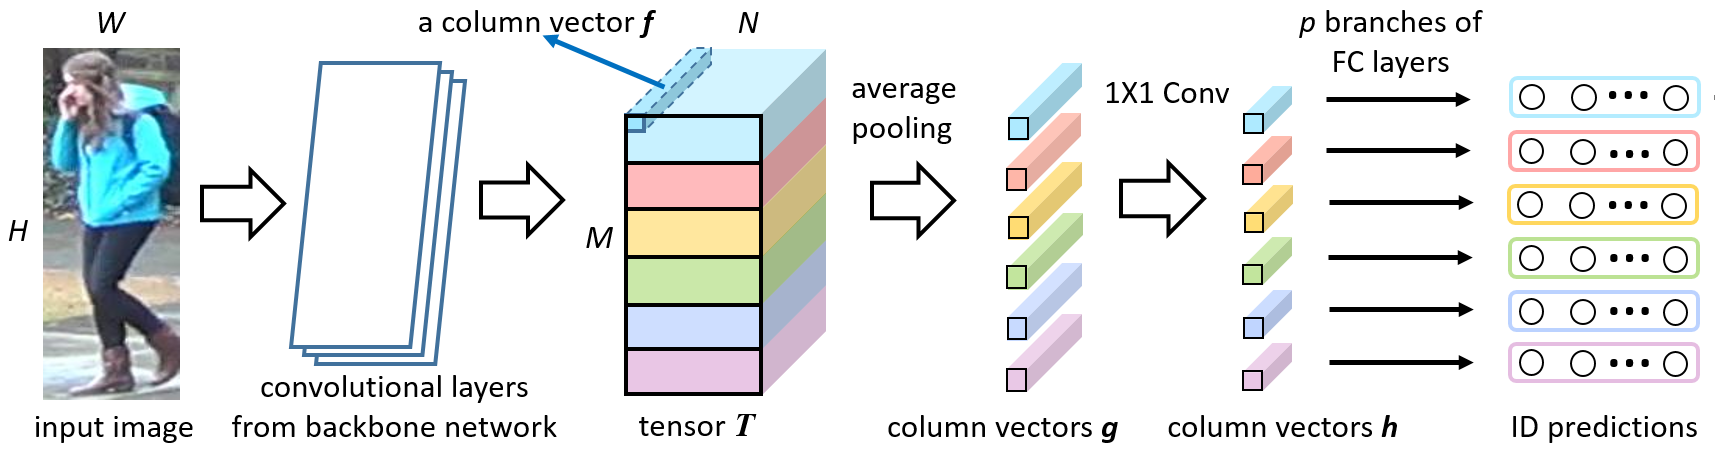
\includegraphics[width=1\textwidth]{structure}
\caption{Baseline架构图}
\label{fig:baseline}
\end{figure}

\section{监控摄像头部署方案的评价指标}
监控摄像头的部署方案包括摄像头的数量以及部署位置。摄像头的部署位置会影响监控场景的完整性、监控画面的光线质量以及监控目标的呈现角度。而监控摄像头数量受成本预算的限制,不可能无限增加,因此在预算有限的约束下,如何设计监控摄像头的部署位置,使得监控效果最优,便成为一个值得研究的问题。而在研究优化问题之前,需要定义监控摄像头部署方案的评价指标。

监控效果的优劣可以定义为在当前的监控方案下,跨摄像头追踪特定行人的能力。当前在多摄像头多行人追踪(Multi-Target Multi-Camera Tracking,Multi-Target Multi-Camera Tracking)领域主流的评价指标有多目标跟踪准确度($\mathit{MOTA}$)和识别F值($\mathit{IDF_1}$)。

\subsection{多目标跟踪准确度($\mathit{MOTA}$)}
多目标跟踪准确度(Multiple Object Tracking Accuracy,$\mathit{MOTA}$)是衡量多目标追踪效果的常见指标。对于一段视频,其画面帧的总数为$T$,那么该段视频的多目标追踪准确度($\mathit{MOTA}$)的定义为:
\begin{equation}
\mathit{MOTA}=1-\frac{\mathit{FP}+\mathit{FN}+\Phi}{T}
\end{equation}
其中$\mathit{FN}$是视频所有帧中将负样本预测为正的总数,$\mathit{FP}$是视频所有帧中将正样本预测为负的总数,$\Phi$是预测序列中标签跳变的次数。MOTA指标的值域为$(-\infty,1]$,越接近1代表跟踪的效果越好。

\begin{figure}
\centering
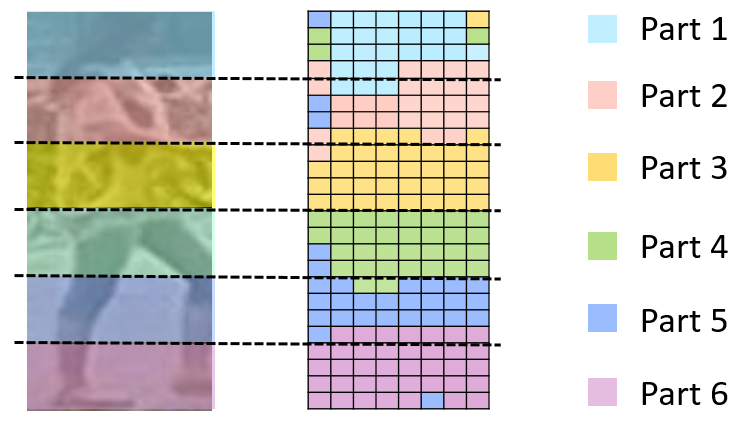
\includegraphics[width=0.6\textwidth]{outliers1}
\caption{Refined Part Pooling示意图}
\label{fig:refined}
\end{figure}

\begin{figure}
\centering
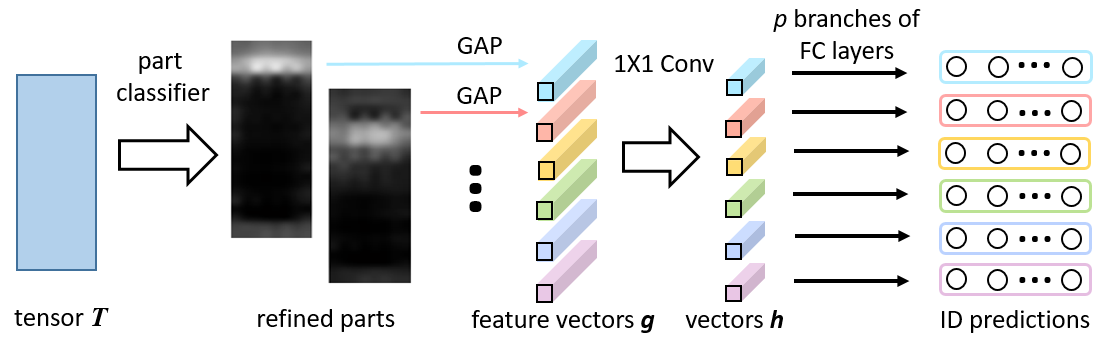
\includegraphics[width=1\textwidth]{structure2}
\caption{PCB+RPP架构图}
\label{fig:structure2}
\end{figure}

\subsection{识别F值($\mathit{IDF_1}$)}
相比与$\mathit{MOTA}$中更多地关注目标人群的召回率以及目标追踪的稳定性,识别F值(Identification F-Score,$\mathit{IDF_1}$)更关注多摄像头多行人追踪过程中,行人标签的准确率。对于一段总帧数为$T$的视频,其识别F值($\mathit{IDF_1}$)定义为:
\begin{equation}
\mathit{IDF_1}=\frac{2\times\mathit{IDTP}}{2\times\mathit{IDTP}+\mathit{IDFP}+\mathit{IDFN}}
\end{equation}
其中$\mathit{IDTP}$是视频所有帧中将人物标签预测准确的总和,$\mathit{IDFP}$是视频所有帧中将正样本的人物标签预测错误的总和,$\mathit{IDFN}$是视频所有帧中将负样本的人物标签预测错误的总和。

\subsection{评价指标与当前的数据库结合}
结合本项目的实际情况,以及第一次预拍摄收集到的数据集的特点,将原始的17个摄像头中的第1个作为行人重识别算法的图库图片来源,其余16个摄像头按照物理位置和拍摄画面分为$G=5$组,每组摄像头个数为2至4个不等,定义$N=16$为待分配的摄像头总数,第$i$组的摄像头个数为$C_i$,同一组内摄像头大致拍摄到同一个物理位置,代表人物监控追踪场景中重点关注的位置。第$i$组的第$j$个摄像头定义为$c_{i,j}$,摄像头$c_{i,j}$的画面帧集合为$I_{c_{i,j}}$。假设在预算有限的前提下,每个位置(每个分组)只能选择1个摄像头,如何从组内选择合适的摄像头,使得监控效果最佳,便是需要解决的问题。该优化问题可以用数学语言形式化表示为:
\begin{equation}
\max \left\{\mathop{\rm eval}\left(\sum_{i=1}^G I_{c_{i,j}}\right)\,\middle\vert\, 1\leq i \leq G, 1\leq j \leq C_i\right\}
\end{equation}
其中$I_1+I_2$表示摄像头1的视频数据与摄像头2的视频数据在时序上依次拼接。$\mathop{\rm eval}(I)$表示对视频数据$I$做多目标跟踪准确度($\mathit{MOTA}$)或识别F值($\mathit{IDF_1}$)评估。

\section{强化学习模型}
强化学习(Reinforcement Learning)是近年来十分流行的人工智能算法,相比于监督学习(Supervised Learning),强化学习不需要整个环境(Environment)所有情况的监督信息,只需要环境在某种特定的情况下给出相应的反馈(Reward)。在很多现实问题当中,优化空间的状态个数可能是个非常大的数字,且很证明是否收集到足够多样本,可以用来近似代表位置环境状态的分布。同时,在围棋问题中\cite{silver2016mastering},各状态空间很难用监督的方法给每个状态评估价值,而强化学习只需要环境在每次动作(Action)之后给出相应的反馈,即可逐渐向更优的方向前进。强化学习也不属于无监督学习(Unsupervised Learning),无监督学习对于出现在测试集却不在训练集的样本没有处理能力,只能错误地分到已有的类中,而强化学习可以应对没有遇到的情况。

强化学习模型中的一般形式是一个智能体(Agent)在一个客观的环境(Environment)中,每一个时刻处于一个状态(State),当前状态存在一个短期价值和长期价值,短期价值可以是采取某种动作(Action)之后得到的反馈(Reward),长期价值(Value)则表示当前状态到最终状态能够得到的所有反馈总和的最大值。智能体根据当前状态的短期或长期价值和某种策略(Policy)采取某种动作,可立刻得到得到环境的反馈(Reward),并据此按照状态转移规则转移到下一个状态。在本项目中,根据要解决的具体问题,将上述概念相应定义如下:

当前的状态的集合$S=\left\{\boldsymbol{s}\,\middle\vert\,\boldsymbol{s}\in\mathbb{R}^{N}, s_i\in\{0, 1\}\right\}$,其中$s_i=1$表示选择了第$i$个摄像头。智能体可以采取的动作集合为$A=\left\{\boldsymbol{a}\,\middle\vert\,\boldsymbol{a}\in\mathbb{R}^N,\boldsymbol{a}_i \in \{0,1\}\right\}$,按照策略 $P$ 来选择动作, 1 表示选择该摄像头,0表示不选该摄像头。在本项目中,进行了动作之后, 状态是确定的,不存在一个动作可能导致几个不同的后续状态的情况,即状态转移概率 $\pi\left(\boldsymbol{s}^t\,\middle\vert\,\boldsymbol{s}^{t-1}, \boldsymbol{a}\right)\equiv1$。执行动作之后得到的反馈$r=\mathop{\rm{eval}}\left(I^{(t+1)}\right)-\mathop{\rm{eval}}\left(I^{(t)}\right)$,其中$I^{(t)}$表示$t$时刻的视频数据,由$t$时刻的状态$\boldsymbol{s}^{(t)}$决定。当前状态 $S$ 的长期价值$V:S\to \mathbb{R}^N$,是一个可学习的变量,代表智能体对于当前环境的认识程度。智能体应对当前状态的策略$P:V \to A$,是长期价值 $V$ 到动作 $A$ 的映射,可以简单地用贪心的策略,即选择概率最高的 5 个摄像头。也可以用 Policy Network ,即深度神经网络来实现。在本项目中采用简单的贪心策略实现。

按照以上定义,智能体的一个动作就是选择一个合法的摄像头部署方案。对于一个动作,它的反馈就是下一个状态的性能指标($\mathit{MOTA}$ 或 $\mathit{IDF_1}$)减去当前状态的性能指标。在反馈已知的前提下,适合用 Q-Learning\cite{watkins1989learning} 算法。在Q-Learning算法中,智能体关于当前状态的长期价值表示为一个价值矩阵$Q$。Q-Learning算法首先随机初始化各个状态的长期价值,让智能体在环境中随机游走,每走一步会得到一个反馈,根据反馈更新当前状态的长期价值,直到收敛。智能体从而可学习出一个对于该环境的认知。本项目中使用Q-Learning算法求当前状态的长期价值如算法\ref{alg:qlearning}所示,其中最关键的算法在于如何更新长期价值$Q$,更新的公式中包含两个参数学习率$\alpha$和远见性$\gamma$,学习率$\alpha$表示$Q$的更新速度,远见性$\gamma$的取值范围为$(0, 1)$,表示智能体对于当前反馈与长远价值的重视程度,$\gamma$越大,代表越重视长远价值。

\begin{algorithm}
    \caption{Q-Learning 算法求当前状态的长期价值}
    \label{alg:qlearning}
    \begin{algorithmic}[1]
        \Require 状态集合$S$、动作集合$A$、生命周期数$N$、学习率$\alpha$、远见性$\gamma$
        \Ensure 长期价值矩阵$Q$
        \Function {QLearning}{$S, A, N, \alpha, \gamma$}
            \State 随机初始化长期价值矩阵$Q$
            \For{$i=0\to N$}
                \State $\boldsymbol{s}^{(0)}\gets\boldsymbol{s}^\star$,$\boldsymbol{s}^\star$为从状态集合$S$中随机初始化的智能体的状态
                \State $t\gets1$
                \Repeat
                    \State $\boldsymbol{a}^{(t)}\gets \boldsymbol{a}^\star$,$\boldsymbol{a}^\star$为从动作集合$A$中随机选取的动作
                    \State $\boldsymbol{s}^{(t+1)}\gets \pi\left(\boldsymbol{s}^{(t)}, \boldsymbol{a}^{(t)}\right)$
                    \State $r^{(t)}\gets R\left(\boldsymbol{s}^{(t+1)},\boldsymbol{s}^{(t)}\right)$
                    \State $Q\left(\boldsymbol{s}^{(t)},\boldsymbol{a}^{(t)}\right)\gets(1-\alpha)\times Q\left(\boldsymbol{s}^{(t)},\boldsymbol{a}^{(t)}\right)+\alpha\times\left[r^{(t)}+\gamma\times\max_{\boldsymbol{a}'}Q\left(\boldsymbol{s}^{(t+1)}, \boldsymbol{a}'\right)\right]$
                    \State $\boldsymbol{s}^{(t)}\gets\boldsymbol{s}^{(t+1)}$
                    \State $t\gets  t+1$
                \Until{$\boldsymbol{s}^{(t)}=\boldsymbol{s}^{(0)}$}
            \EndFor
            \State\Return $Q$
        \EndFunction
    \end{algorithmic}
\end{algorithm}

\section{面向CPU集群的分布式深度学习训练框架}

\begin{figure}
\centering
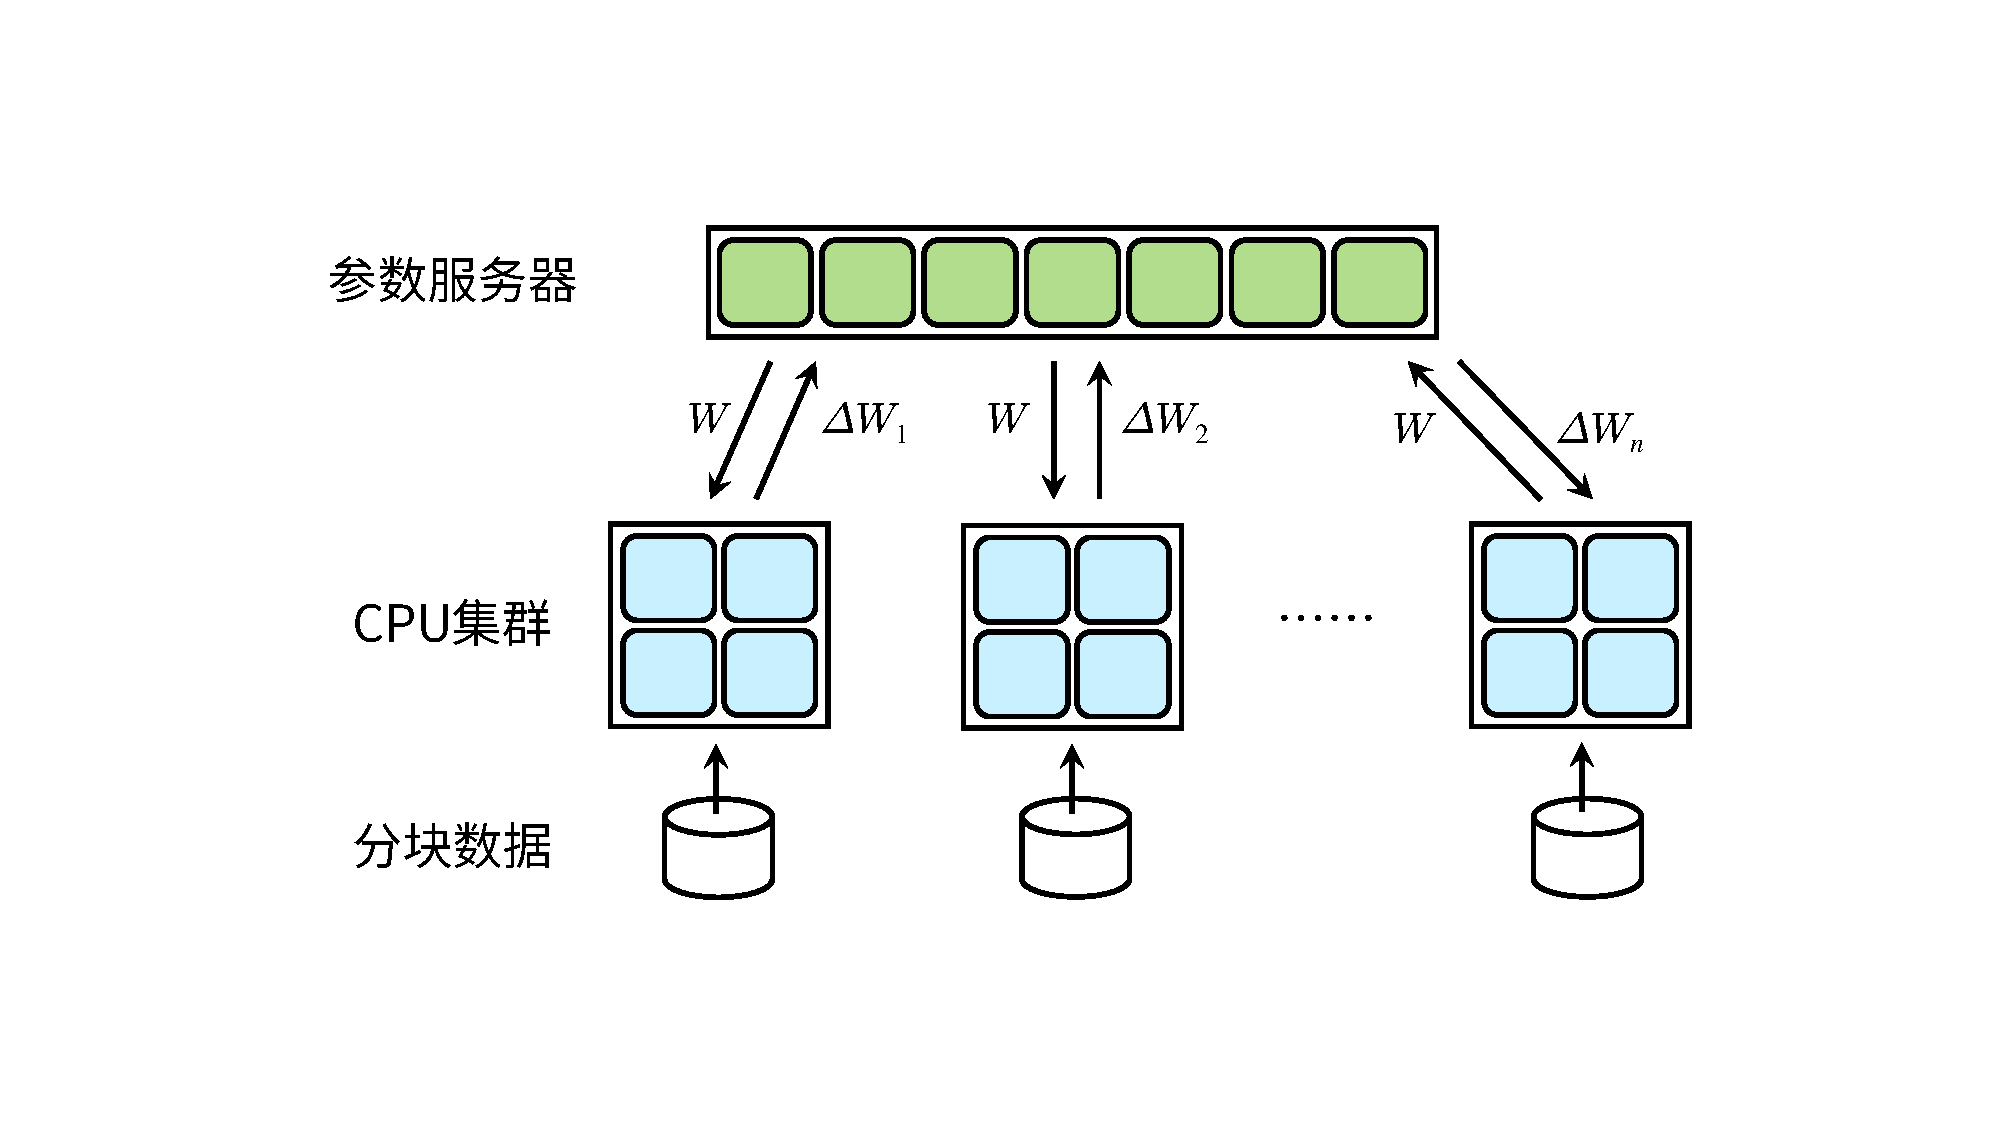
\includegraphics[width=0.7\textwidth]{dist}
\caption{分布式神经网络训练架构图}
\label{fig:dist}
\end{figure}

计算机集群是一种计算机组织的物理形态,它是由一组彼此连接的计算机组成的,这些计算机一般协同完成同一项计算任务。在同一集群中每台计算机的内部结构可以不同,特别地,若集群中每台计算机主要的算力提供者是CPU,那么称该集群为CPU集群。分布式计算是计算的一种工作方式,它将一个计算任务划分成多个子任务,每一个子任务与其它子任务相对独立,可以在时间上并行计算,以缩短计算时间。CPU集群提供了一组在物理上相对独立的计算机,所以可以很自然地考虑将分布式计算中的各个子任务部署到CPU集群中,充分利用CPU集群的计算资源。

深度神经网络模型的训练过程一般可分为前向计算(Forward)、误差反向传播(Loss Backpropagation)和参数更新。其中前向计算和反向传播的计算量很大,而且可以针对不同的训练集进行同步计算,因此深度神经网络模型的训练过程在结构上很适合进行分布式训练。在本项目中,集群的数量$n=5$,每个节点属于天河二号的GPU分区,具备高性能的CPU和GPU计算资源,节点之间通过千兆网络连接,避免各节点的通信速度成为分布式计算的性能瓶颈。

分布式训练架构如图\ref{fig:dist}所示,将训练数据通过随机采样的方式平均分成$n$份,分别输入集群中的各计算机。每一台计算机内存中包含一个独立的深度神经网络模型,进行该份训练数据的前向计算和反向传播计算,得到该批次训练数据在当前模型下的各参数梯度。参数服务器的计算任务是收集集群中各计算机回传的梯度,更新模型参数,并将新参数分发给各计算机,各计算机得到新参数后进行下一批次训练数据的计算。更新模型参数的方法为:
\begin{eqnarray}
\Delta W=\frac{1}{n}\sum_{i = 1}^{n}\Delta W_i \\
W=W-\eta\Delta W
\end{eqnarray}
其中$\eta$是参数的学习率。

        % 算法实现
        \chapter{项目内容及算法实现}\label{sec:algorithm}

本章介绍了项目在准备阶段和项目主体部分各算法的实现细节。项目的准备阶段包括原始视频处理、行人检测以及人工标注行人标签。项目的主体部分包括行人重识别算法的复现、多CPU集群分布式训练的实现以及强化学习算法的实现。

\section{数据采集和预处理}

\subsection{数据采集}

经过路线规划、场地布置、演员召集等工作,完成了数据库第一次预拍摄以及正式拍摄工作。数据集的正式拍摄于 2018 年 5 月 19 日和 20 日进行,召集了 500 余名演员,实际到场的人数为463人。由于正式拍摄的视频数据还需要长时间的整理和标注,所以本项目使用第一次预拍摄数据作为目标数据集$\mathcal{D}^{des}$。第一次预拍摄过程的详细情况如下:

第一次预拍摄的参与者为 19 人,其中有 15 人完整地走完了路线,全程拍摄时长大约为 25 分钟。视频拍摄的地点位于中山大学数据科学与计算机学院楼外停车场与楼内 1、2、3、4、6 楼的大厅和走廊。视频拍摄过程中需要在若干个关键点(某个摄像头或者某一楼层)设置人员负责时间点记录和人流控制,记下每一个演员进入视频画面的时间点,用于之后的视频分割。

第一次预拍摄一共使用了 21 个摄像头,最终 20 个摄像头有视频输出。视频的分辨率为1920$\times$1080(1080P)或1280$\times$720(720P),帧率均为 25 FPS。最终用于本项目的数据集包含 17 个摄像头的视频数据,每个摄像头的视频数据包含在一个视频文件内,视频的长度约为 10 分钟,出现的演员有 15 人。

\subsection{原始视频处理}

\subsubsection{视频转码}

由于拍摄设备的规格不一致,且设备编码视频的质量也参差不齐,出现了许多问题:原有的摄像头输出的视频文件的时间轴有误,原本时长为 20 分钟的视频却显示有 13 个小时。部分原始视频文件偶尔会出现一两帧丢失的情况,不是准确的 25 FPS。原始视频被分割成了 2 $\sim$ 3 个视频文件。因此需要用 FFmpeg 对原始视频进行转码。转码保持原有的分辨率不变,填补少量的丢失帧,修正视频的时间轴信息、文件头信息,拼接多个视频,将音频轨道删除,最终输出正常的视频文件。此阶段的输出是:每个摄像头对应一个视频文件。

\subsubsection{时间点校正和估计}

在视频拍摄过程中需要多名记录员记录演员进入视频画面的时间点和演员的标签,以便后期的视频处理。将记录员记录的第一个时间点与视频中第一个演员出现的时间点对齐,即可得到每个演员进入视频画面的时间点。对于那些没有记录员的摄像头,则采用“进入上一个摄像头的时间 + 两摄像头之间平均行走时间”的方法来估计。由于记录的时间并不是完全准确,且估计的结果也不是完全精确,所以有部分的记录数据需要对照视频重新调整时间点。此阶段的输出是:每一个演员的进入每一个摄像头的时间点。

\subsubsection{视频切割}

有了每一个演员演员进入每一个摄像头的时间点,然后再分别估计每一个摄像头画面中演员停留的平均时间,即可得到每一个演员在每一个视频文件中的时间段,从而利用 FFmpeg 将每一个演员在没一个摄像头的视频片断切割出来。此阶段的输出是:每个演员在每个摄像头的视频片断。

\subsection{行人检测}

行人检测属于计算机视觉领域中的目标识别(Object Detection)问题,目前目标识别问题state-of-the-art 是何凯明等人的Mask RCNN~\cite{he2017mask}模型。Mask RCNN在Faster RCNN~\cite{ren2015faster}的基础上,添加了一条网络分支,以实现在目标检测的同时,将每个像素分割出来,得到高质量的分割结果。

在本项目中,使用了Mask RCNN作者公开的源代码项目Detectron~\cite{Detectron2018}作为行人检测工具,该项目中包含预训练的网络参数和目标检测API,预训练模型在训练过程中使用了COCO 2014~\cite{lin2014microsoft}数据集,模型的后端深度神经网络使用了ResNet-101~\cite{he2016deep}网络。

对于每个视频文件,遍历其所有的画面帧,调用Detectron API检测画面当中的行人,再根据记录员的记录得到画面中行人的标签。由于画面中可能存在多于一个行人,所以此步骤会将不属于演员的路人也打上演员的标签,需要后期的修正。对于画面中的每一个行人,输出一条记录,其包含的字段分别为:摄像头ID、演员ID、当前帧数、当前帧内行人个数、Bounding Box的左上角与右下角坐标、行人的概率。

\subsection{人工标记行人的标签}

由于 Detectron 无法区分在同一帧内的演员和路人,暂时输出了相同的标签,所以需要进一步地用人工把那些路人的标签标记为 -1。

人工标记的过程借助了事先实现的行人重识别模型,具体过程如下:

将记录中当前帧内行人个数为1的记录挑选出来并按照标签分组,由于该帧中行人数量为 1,所以可以确定当中行人标签的正确性。把每个 Bounding Box 输入行人重识别模型,得到该人的特征。再求标签相同的特征的均值,得到可以代表每一个演员的特征向量。

对于记录中当前帧内行人个数大于1的部分,按照摄像头ID、标签、当前帧数分组,每一组内就是同一摄像头下同一帧内的所有行人的记录。计算每个行人的特征向量与该标签演员的特征向量之间的距离,将距离最近的那条记录的标签标记不变,其它记录的标签改为-1。此时每一个当前帧内行人个数大于1的组内只有一条记录的标签不为-1。

将每个组内标签不为 -1 的图像输出文件,摄像头ID及标签相同的图片放入同一个文件夹,人工评估每个文件夹内的标注结果。删除标注出错的图片,剩余的图片最能代表该场景、该演员的特征,所以求该文件夹内剩余图片的特征向量的均值,作为代表该演员在该场景下的特征向量。

扫描每个文件夹内缺失的图片(文件缺失代表在上一步被删除了,自动标注出错,需要进一步标注),按照与之前步骤类似的做法,找出与对应文件夹内特征向量最近的记录,将其它记录的标签标记为 -1,再次输出图片到文件,人工检查结果。

将每个文件夹内标注出错的结果人工删除。用代码扫描被删除的图片,将原始记录中该帧图像中所有的记录删除。因为到此步骤标注出错的情况很少,所以仅删除了少量的记录,对最终的数据集完整性影响不大。

\section{行人重识别模型复现}

\subsection{读入训练/测试数据}

Market1501数据集的格式是原始的JPG图片,所以需要加载自己的训练集,这种情况下如果使用PyTorch框架,最好还是继承 Dataset 类。Dataset 类的本质是定义了数据所在的位置,以及数据需要预处理的方法。至于数据的位置是在硬盘里面还是提前加载到内存里面,由该类的内部实现决定。由于Market1501数据集过大,所以本项目采用了分批次读取的做法,在训练和测试过程中使用20个进程将数据从硬盘加载到内存中。

\subsection{模型训练}\label{sec:modeltraining}

在本项目中,模型的训练使用了Market1501~\cite{zheng2015scalable}数据集,数据集使用了水平平移翻转和正则化作为数据扩充的方法。训练模型分为三个阶段,第一阶段是标准的PCB训练,即均匀地分割特征图张量的各个部分。此阶段一共包含60个Epoch,Batch Size为64,模型新增的卷积层的参数初始化为服从正态分布$N(0, 0.001^2)$的随机数。ResNet50网络参数的学习率为0.01,其它参数的学习率为0.1,当Epoch大于或等于40时,各学习率分别缩小为初始的$1/10$。训练模型的第二阶段将PCB中均匀分割改为分类,并且固定第一阶段训练的所有参数,只学习分类层的参数,训练的Epoch数和Batch Size与第一阶段相同。分类层的参数同样初始化为服从正态分布$N(0, 0.001^2)$的随机数,初始学习率为0.01,当Epoch大于或等于40时,学习率缩小为初始的$1/10$。训练模型的第三阶段为调整整个网络中所有的参数,训练的Epoch数和Batch Size与第一阶段相同。所有参数的初始学习率为0.01,当Epoch大于或等于40时,学习率缩小为初始的$1/10$。

\subsection{特征提取}

在特征提取阶段,将最后用于分类任务的全连接层移除,并将全连接层移除后网络最后一层或倒数第二层输出的$p$个向量拼接起来,得到行人的特征表示。在测试阶段,采用欧氏距离衡量各特征之间的相似度。

\section{强化学习框架实现}

强化学习框架实现了Q-Learning算法以及监控摄像头部署方案评价指标计算函数。Q-Learning算法的伪代码如算法~\ref{alg:qlearning}~所示,由于逻辑比较简单,所以没有利用现有的深度强化学习框架,而是使用基本的\texttt{numpy}库实现。监控摄像头部署方案评估指标$\mathcal{E}$选择了$\mathit{MOTA}$的值,计算方法如式~\ref{eq:mota}~所示,在实现过程中使用了\texttt{PyTorch}的API。在Q-Learning算法中,智能体的生命周期数$N$为100000,状态的长期价值$Q$的学习率$\alpha$为0.01,智能体的远见性$\gamma$为0.2。

\section{面向多CPU集群的分布式深度学习训练框架}

将原本只能单机训练的深度学习模型改造成能够在多CPU集群上运行的分布式深度学习模型,经历了以下过程:

\begin{enumerate}
    \item 实现数据分组策略算法,在每一个Epoch中,数据分组策略算法需要随机地将整个数据集划分成份数与节点数相同的子数据集,以便在接下来的过程中分发给各节点。
    \item 实现各节点之间通信。在本项目中各节点只需与主节点进行的通信,子节点之间不需要通信,因此只需保证各子节点知道主节点的IP地址,以及主节点监听的端口号,使用TCP协议实现数据通信。
    \item 实现各节点计算过程同步进行。在训练过程中需要保证各节点的Epoch一致性,所以在每次进入一个新Epoch都要跟主节点进行通信,确保各节点当前计算的Epoch一致才进行接下来的计算。在每次误差反向传递之后,各节点都要将本次计算的梯度与主节点同步,主节点根据各梯度更新模型参数。
\end{enumerate}
        % 实验结果
        \chapter{实验结果}\label{sec:experiment}

\section{自采集数据呈现}

本项目中自采集数据分为第一次预拍摄数据Multi-Cameras1和正式拍摄数据Multi-Cameras2,两次拍摄得到的数据集与现有行人重识别领域主流数据集的比较如表\ref{tab:reiddataset}所示。我们的数据集是唯一包含大量持续跟踪行人的数据集,同一行人至少会出现在17个视野不重叠的摄像头视野内,非常适合用于要求更苛刻的行人重识别以及行人追踪任务。需要注意的是,我们现阶段统计的行人数量,只包括完整地出现在所有摄像头内的人数,而实际视频画面中还出现了很多无标签的路人,若为这些路人打上正确的标签,那么数据集中行人数量会大大增加。

\begin{table}[!htb]
\centering
\caption{行人重识别领域常见数据库情况统计}
\label{tab:reiddataset}
\begin{threeparttable}
\begin{tabularx}{\textwidth}{ccccccc}
\toprule
数据集名称   & 公布时间 & 行人数量 & 摄像头数量 & 图片数量  & Multi-shot~\tnote{a} & Tracking~\tnote{b} \\ \midrule
VIPeR\cite{gray2007evaluating}  & 2007 & 632  & 2     & 1264  & 否  & 否 \\
CUHK01\cite{li2012human} & 2012 & 971  & 2     & 3884  & 否  & 否 \\
CUHK03\cite{li2014deepreid} & 2014 & 1467 & 10    & 13164 & 是  & 否 \\
Market1501\cite{zheng2015scalable} & 2015 & 1501 & 6     & 32217 & 是  & 否 \\
DukeMTMC4reID\cite{gou2017dukemtmc4reid}  & 2017 & 1852 & 8     & 46261 & 是  & 否 \\
Multi-Cameras1 &  -~\tnote{c}   & 15~\tnote{d}   & 17     & 98543 & 是  & \textbf{是} \\
Multi-Cameras2 &  -~\tnote{c}   & 463~\tnote{d} & 24     & -~\tnote{e} & 是  & \textbf{是} \\
\bottomrule
\end{tabularx}
\begin{tablenotes}
    \footnotesize
    \item[a] 同一行人是否有超过 2 张图片。
    \item[b] 是否持续追踪同一行人。
    \item[c] 未来会公布数据库,时间待定。
    \item[d] 该数字只包含完整走完全程的演员,还有大量无标签的路人未计入。
    \item[e] 数字具体尚未统计,但预计会远大于100k。
\end{tablenotes}
\end{threeparttable}
\end{table}

\subsection{摄像头分布与分组}

表\ref{tab:cameraslayout}展示了16个摄像头的拍摄画面和分组情况。在本次采集的数据集中一共有5个场景,分别为楼外停车场、一楼庭院、二楼走廊、三楼电梯出口、三楼走廊。这5个地点分布在一条连续路线上,每个地点存在2$\sim$4个摄像头,是十分适合用于研究行人追踪的场景。

从表\ref{tab:cameraslayout}可以看出,相同拍摄地点的不同摄像头所拍摄的画面之间存在较大差异,如角度方面的差异:第2组场景一楼庭院,第1个摄像头拍摄的是行人的正背面,第2个摄像头拍摄的是行人的右俯视角度画面,第3个摄像头拍摄的是行人的左俯视角度画面。光线方面的差异:第3组场景二楼走廊,第1、4个摄像头距离行人很近,但是画面光线很暗,成像质量也很模糊,第2、3个摄像头光线较好。拍摄范围与通过时长的差异:第4组场景三楼电梯,第1、2个摄像头距离电梯门较近,行人出电梯后会在1$\sim$2秒内走出画面范围,因此相比于第3个摄像头所获得的信息相对较少。

\begin{table}[!ht]
\centering
\caption{摄像头拍摄画面及分组}
\label{tab:cameraslayout}
\renewcommand{\arraystretch}{1.5}% Spread rows out...
\begin{tabularx}{\textwidth}{>{\centering\bfseries}m{0.2\textwidth} >{\centering\arraybackslash}m{0.7\textwidth}}
\toprule
分组(场景名称) & \textbf{摄像头画面} \\
\midrule
1. 楼外停车场 & 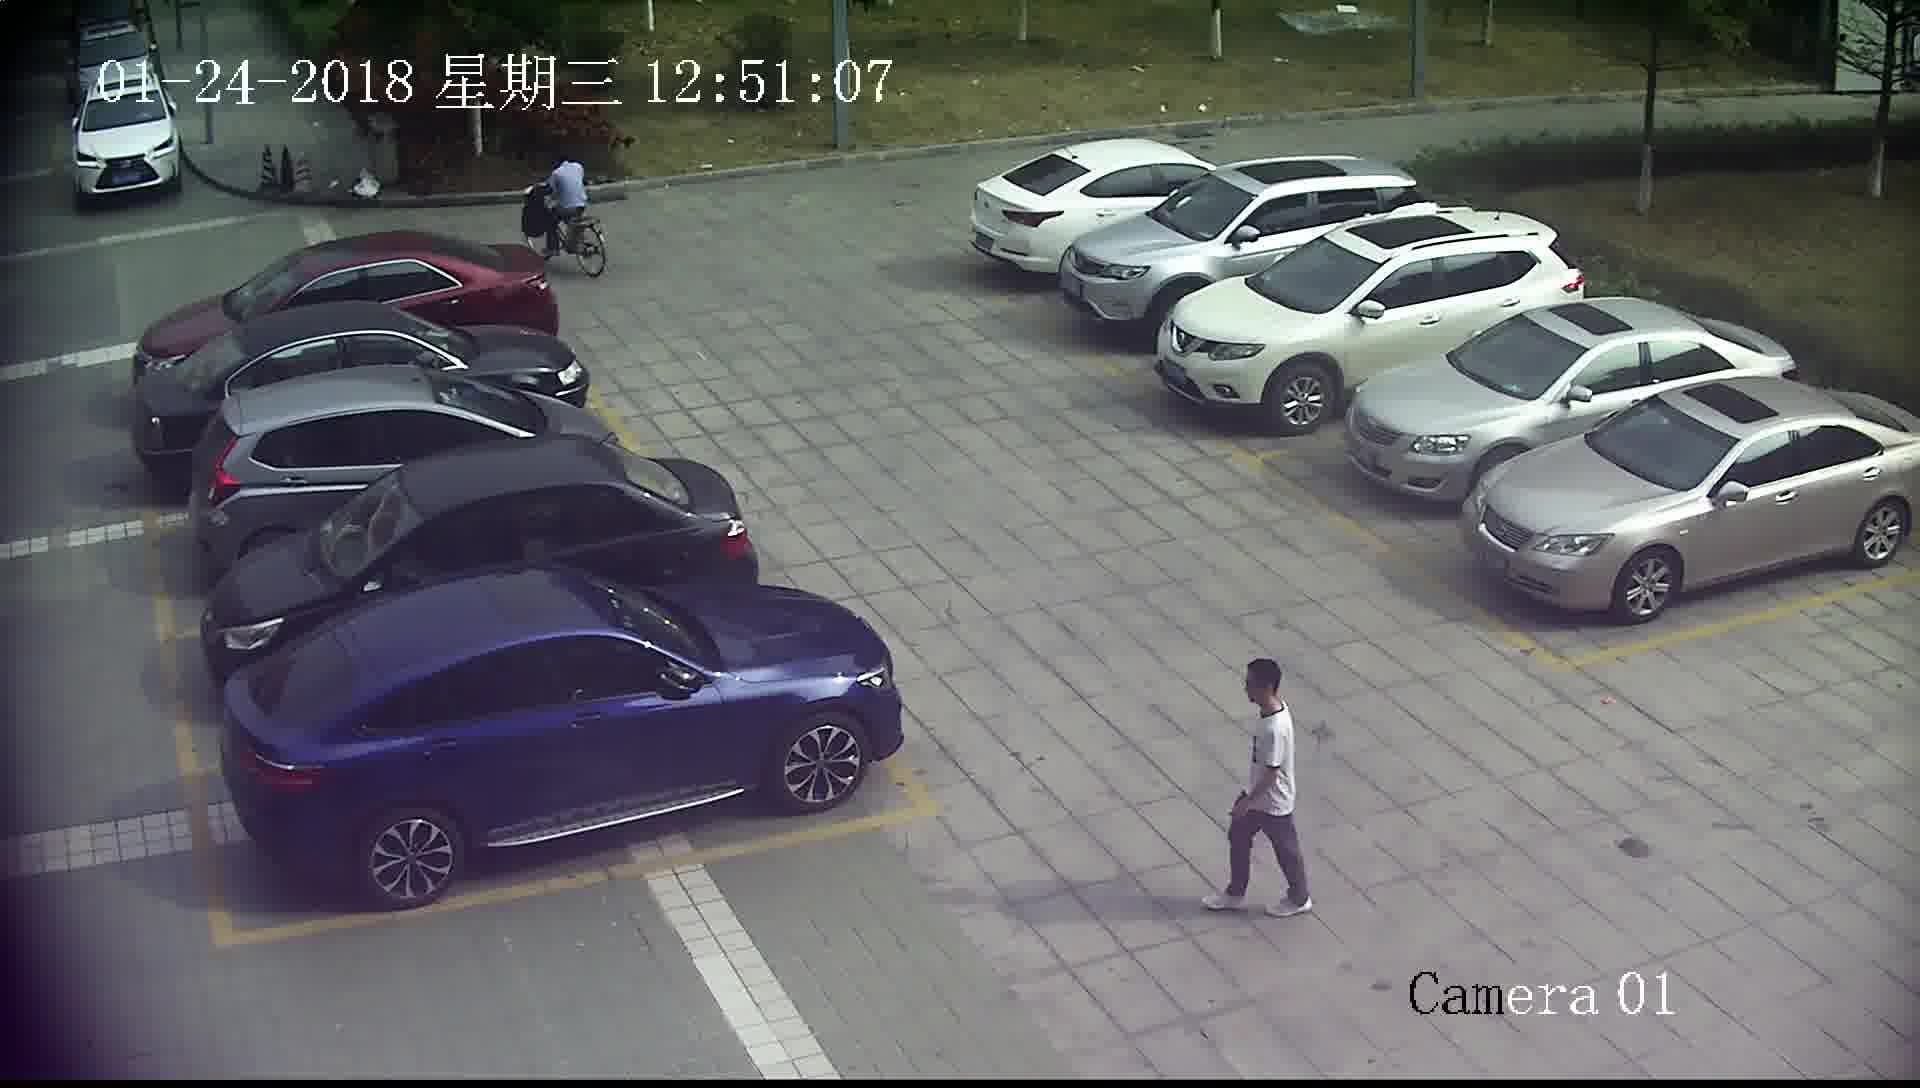
\includegraphics[width=25mm]{1-1}~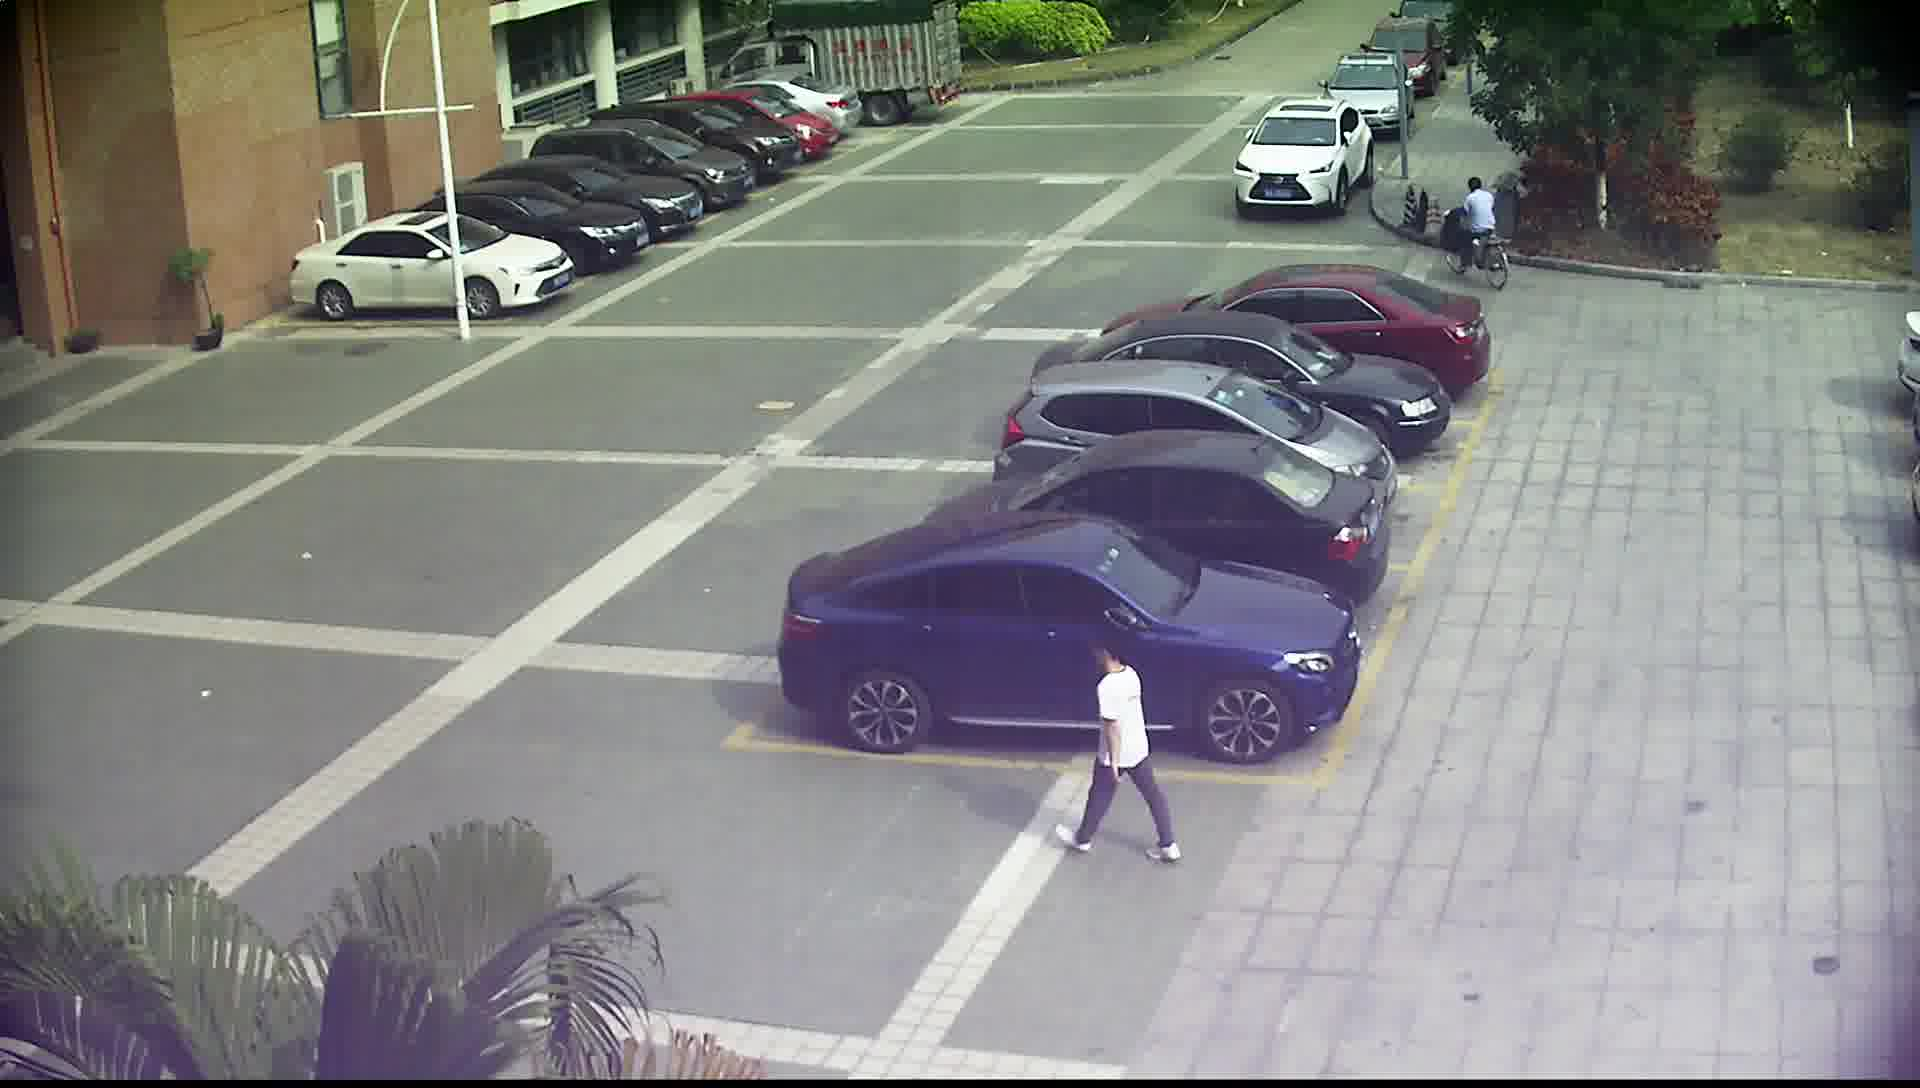
\includegraphics[width=25mm]{1-2} \\
2. 一楼庭院 & 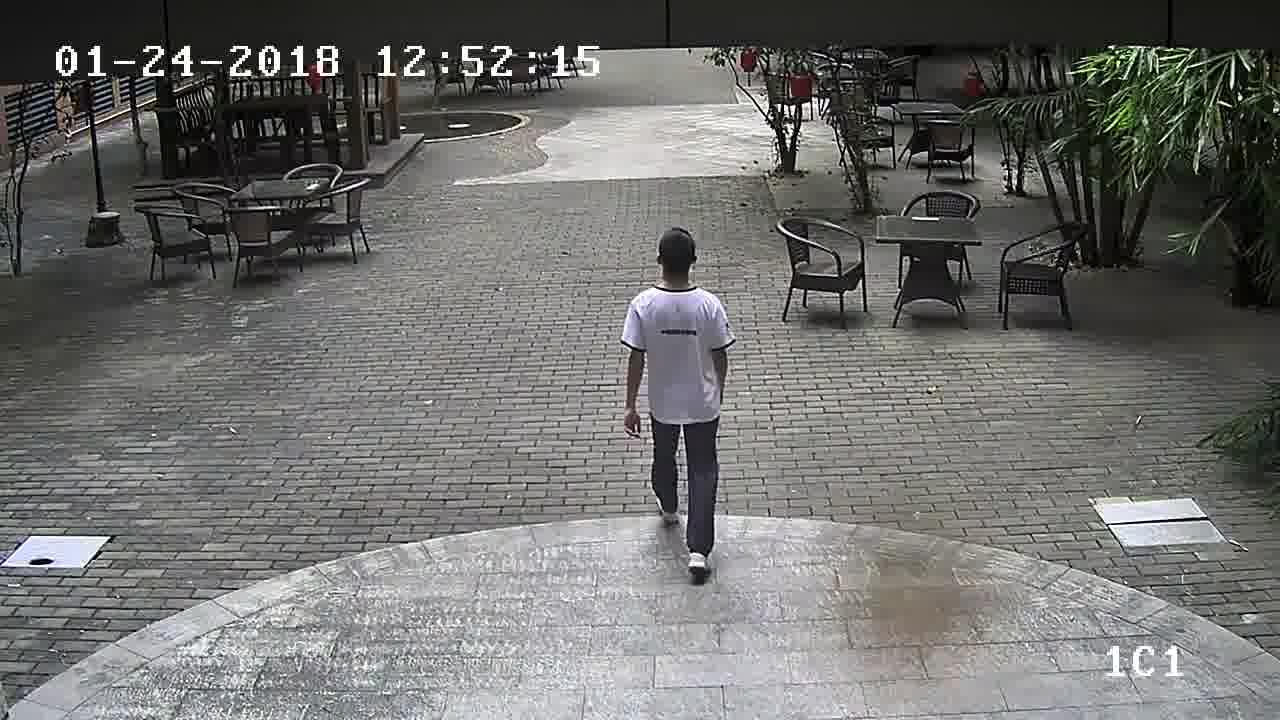
\includegraphics[width=25mm]{1-4}~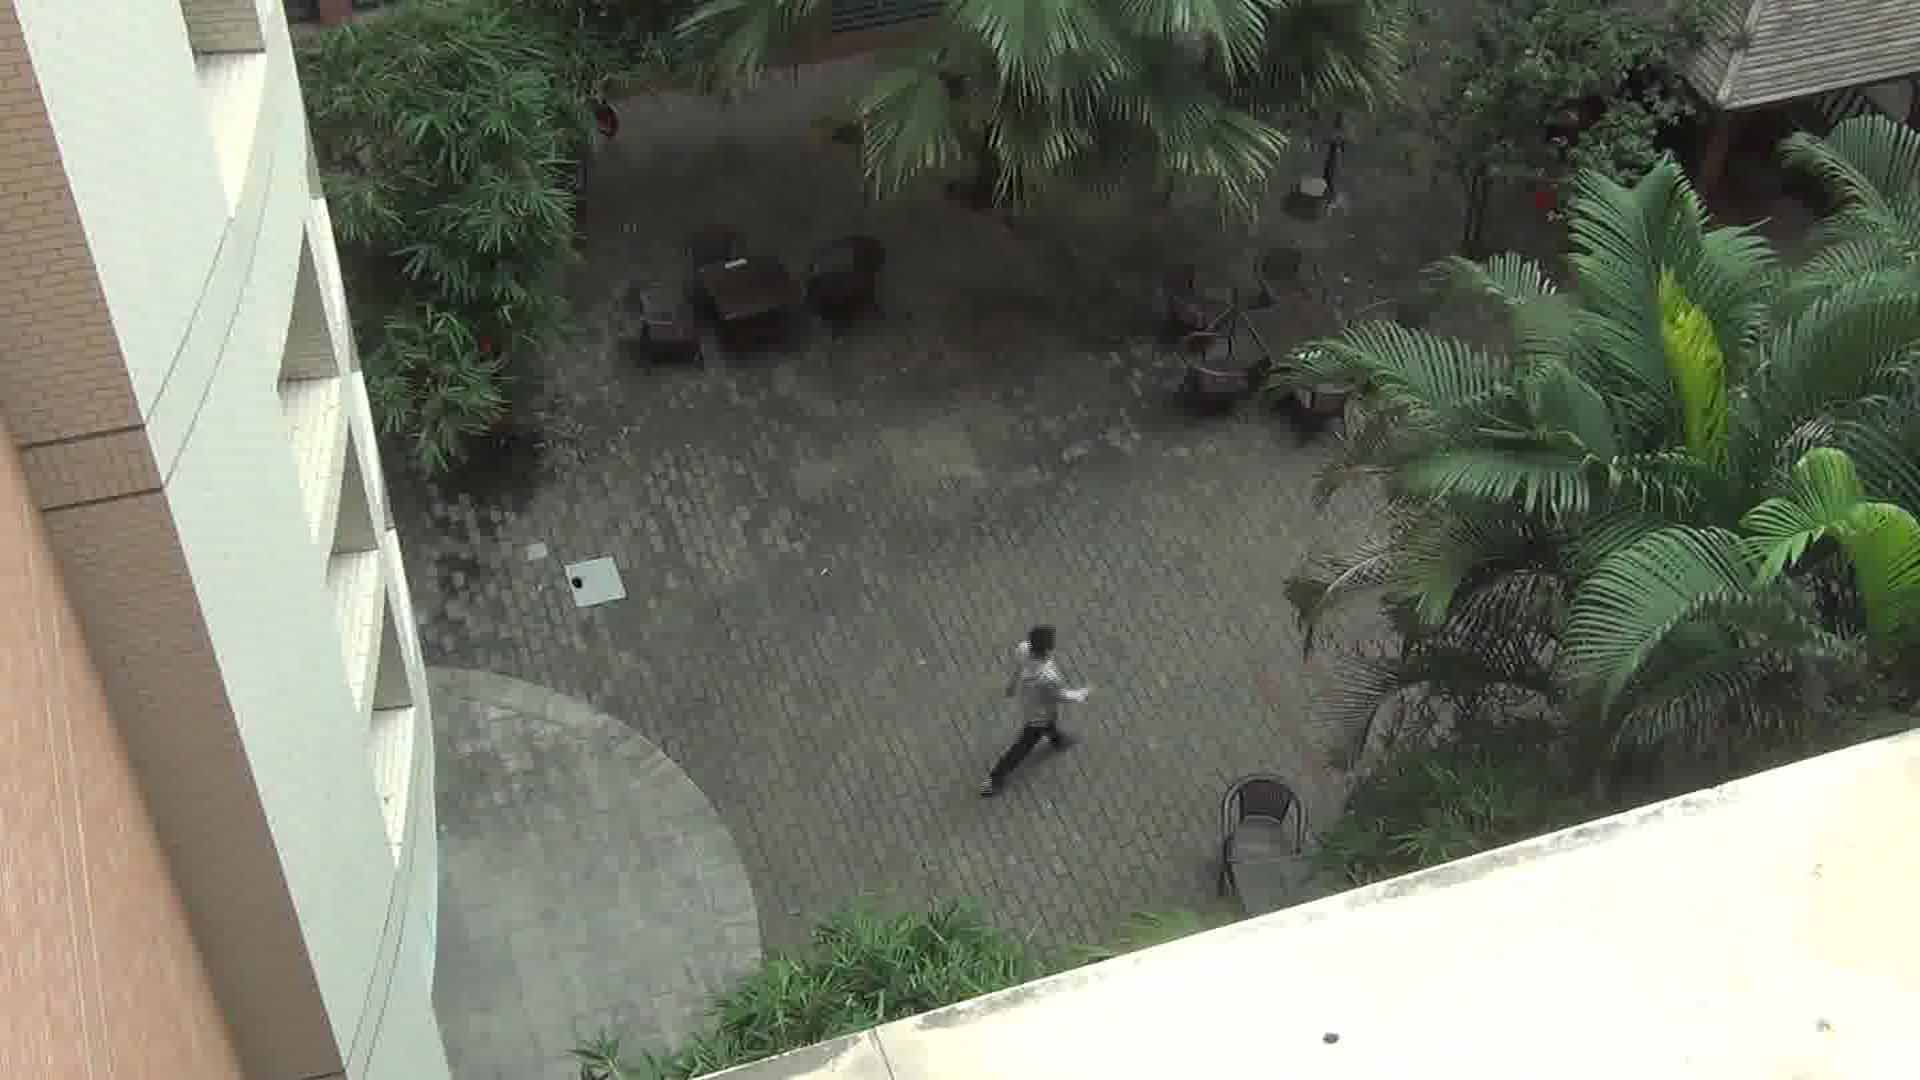
\includegraphics[width=25mm]{1-5}~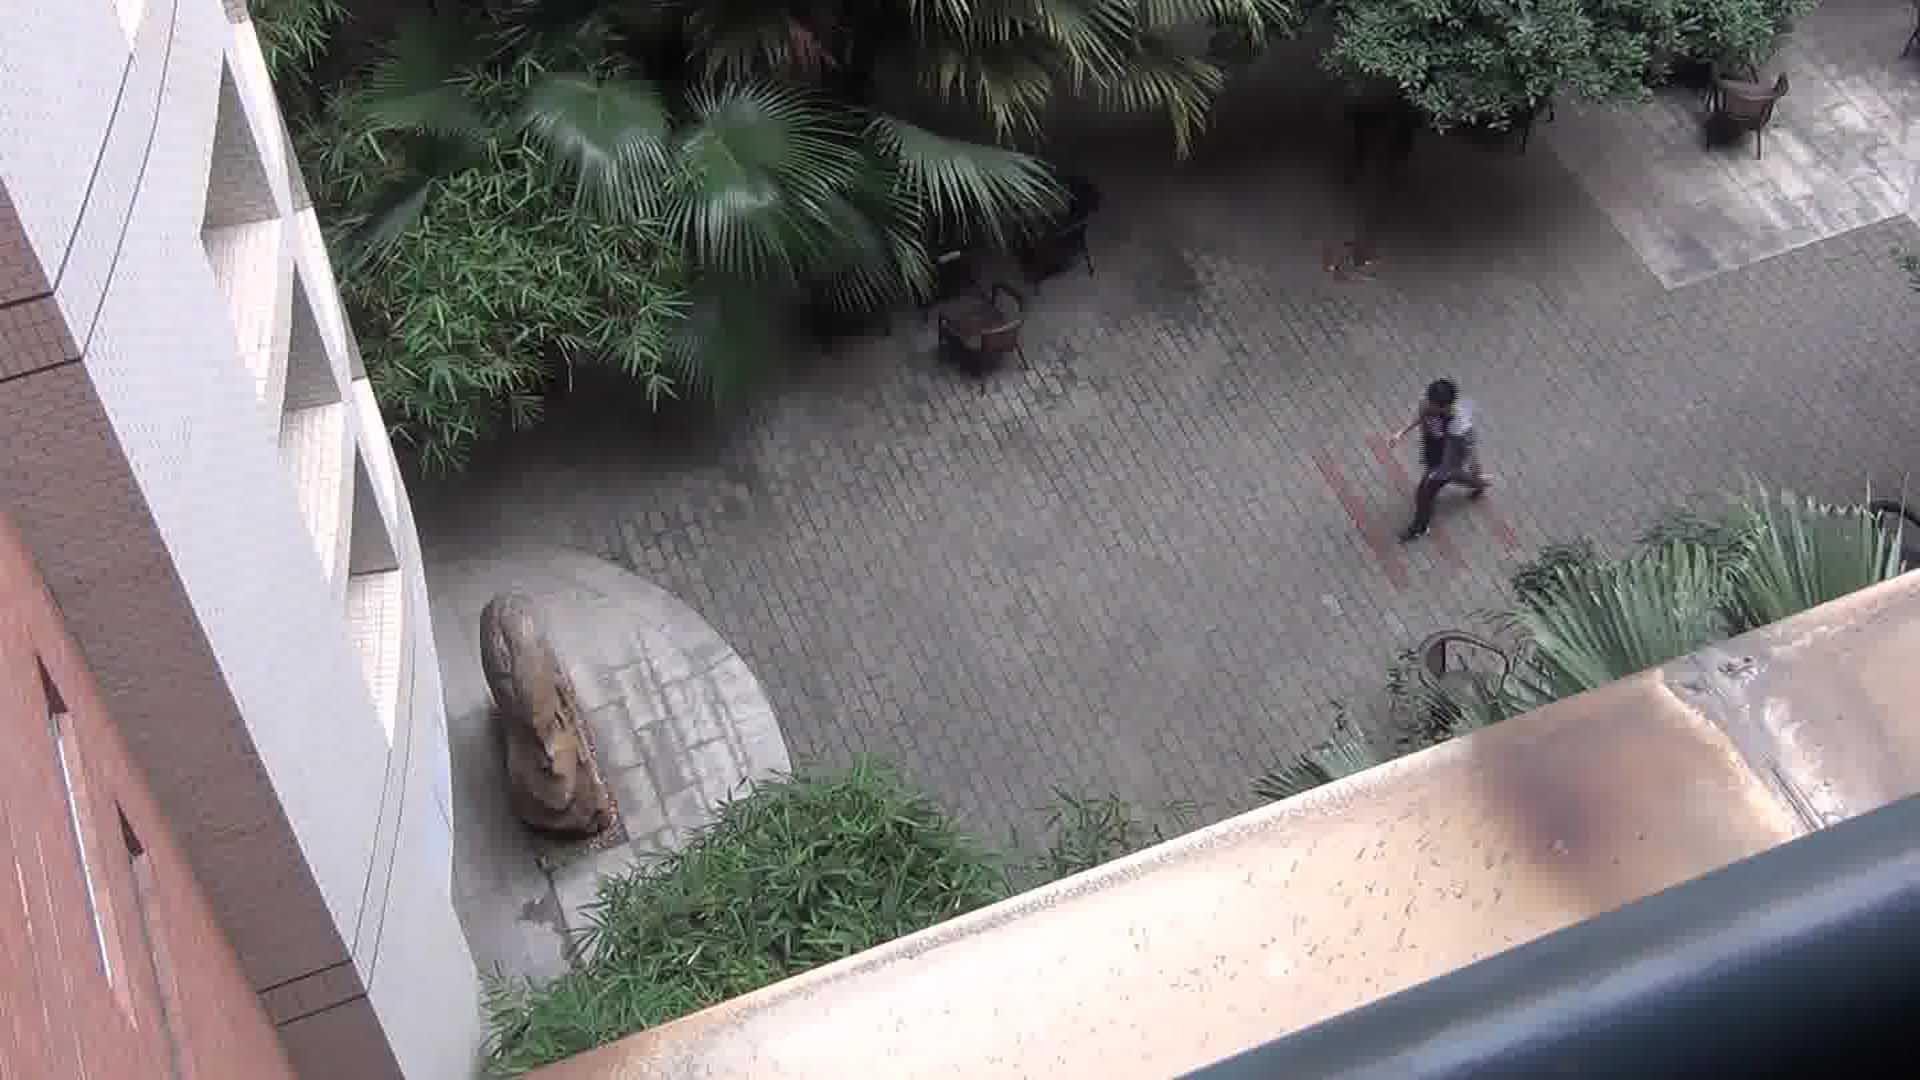
\includegraphics[width=25mm]{1-6} \\
3. 二楼走廊 & 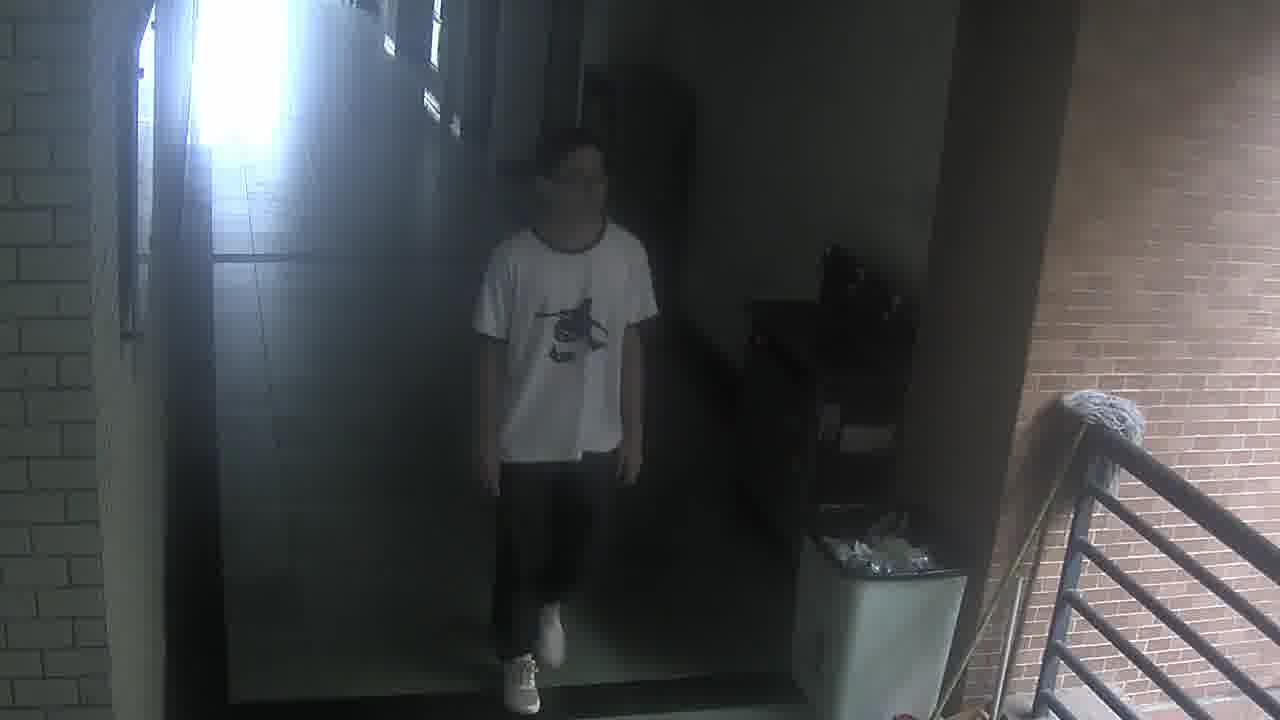
\includegraphics[width=25mm]{2-1}~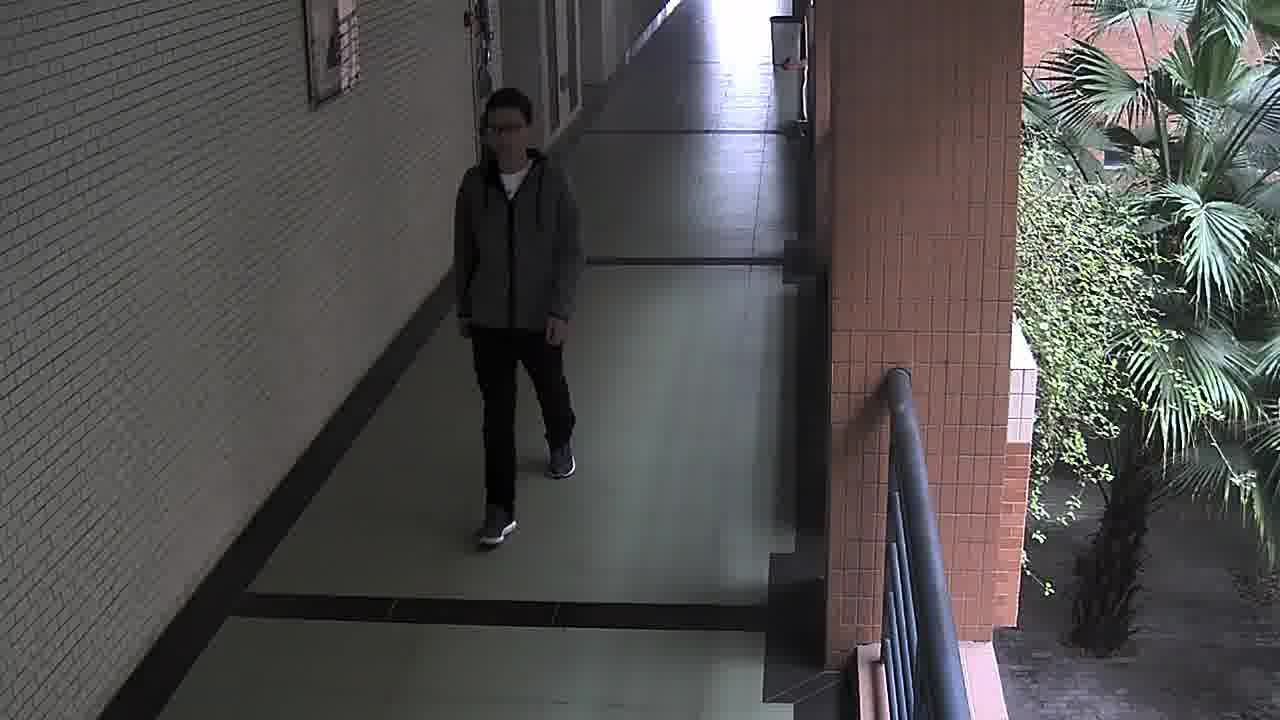
\includegraphics[width=25mm]{2-2}~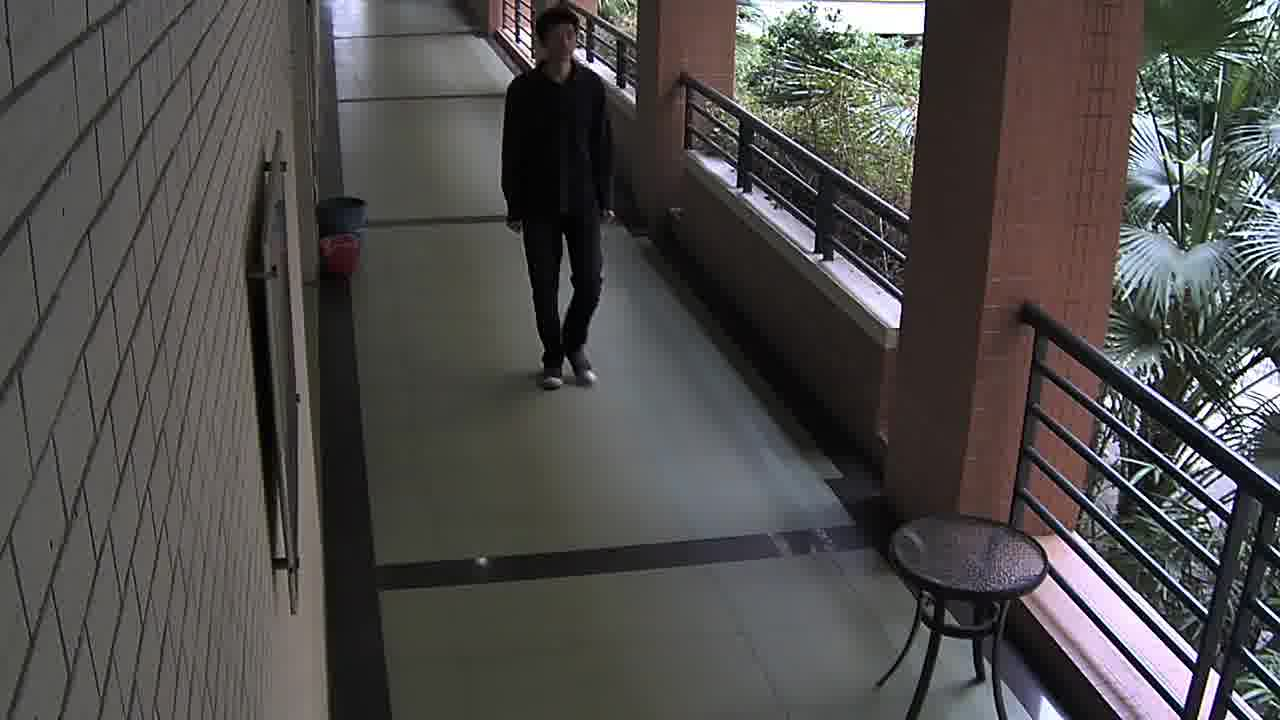
\includegraphics[width=25mm]{2-3}~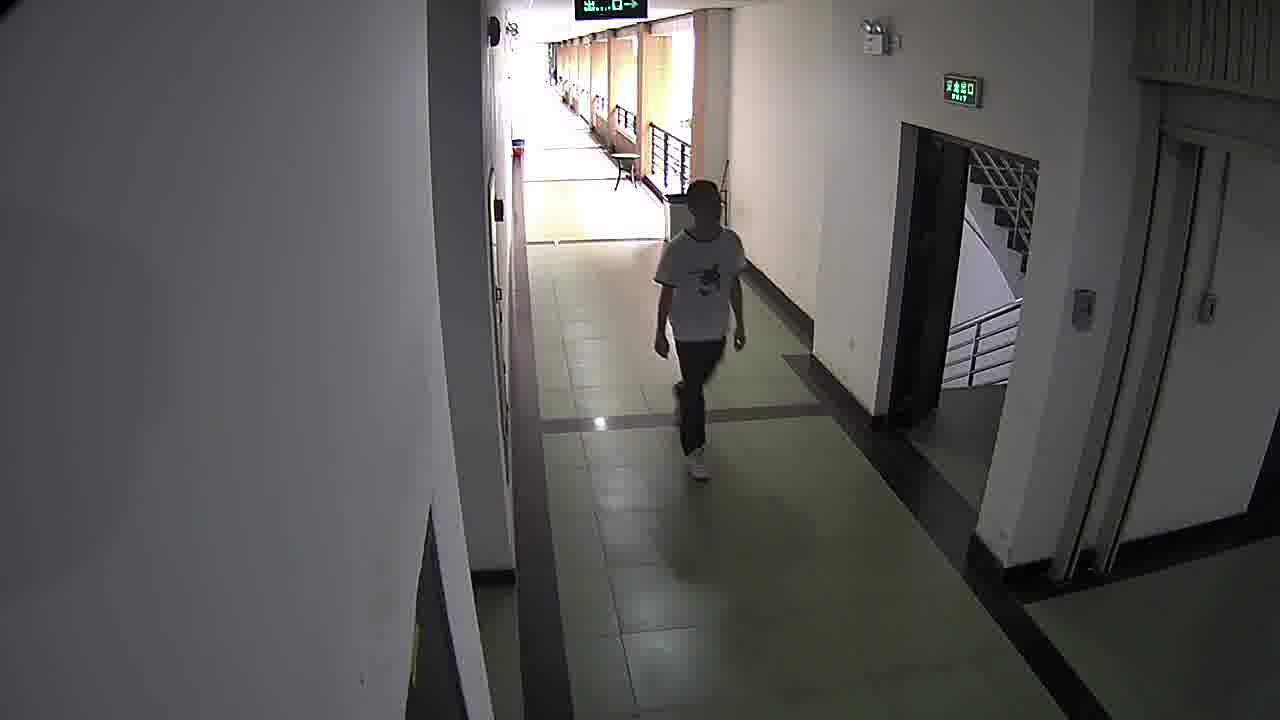
\includegraphics[width=25mm]{2-4} \\
4. 三楼电梯 & 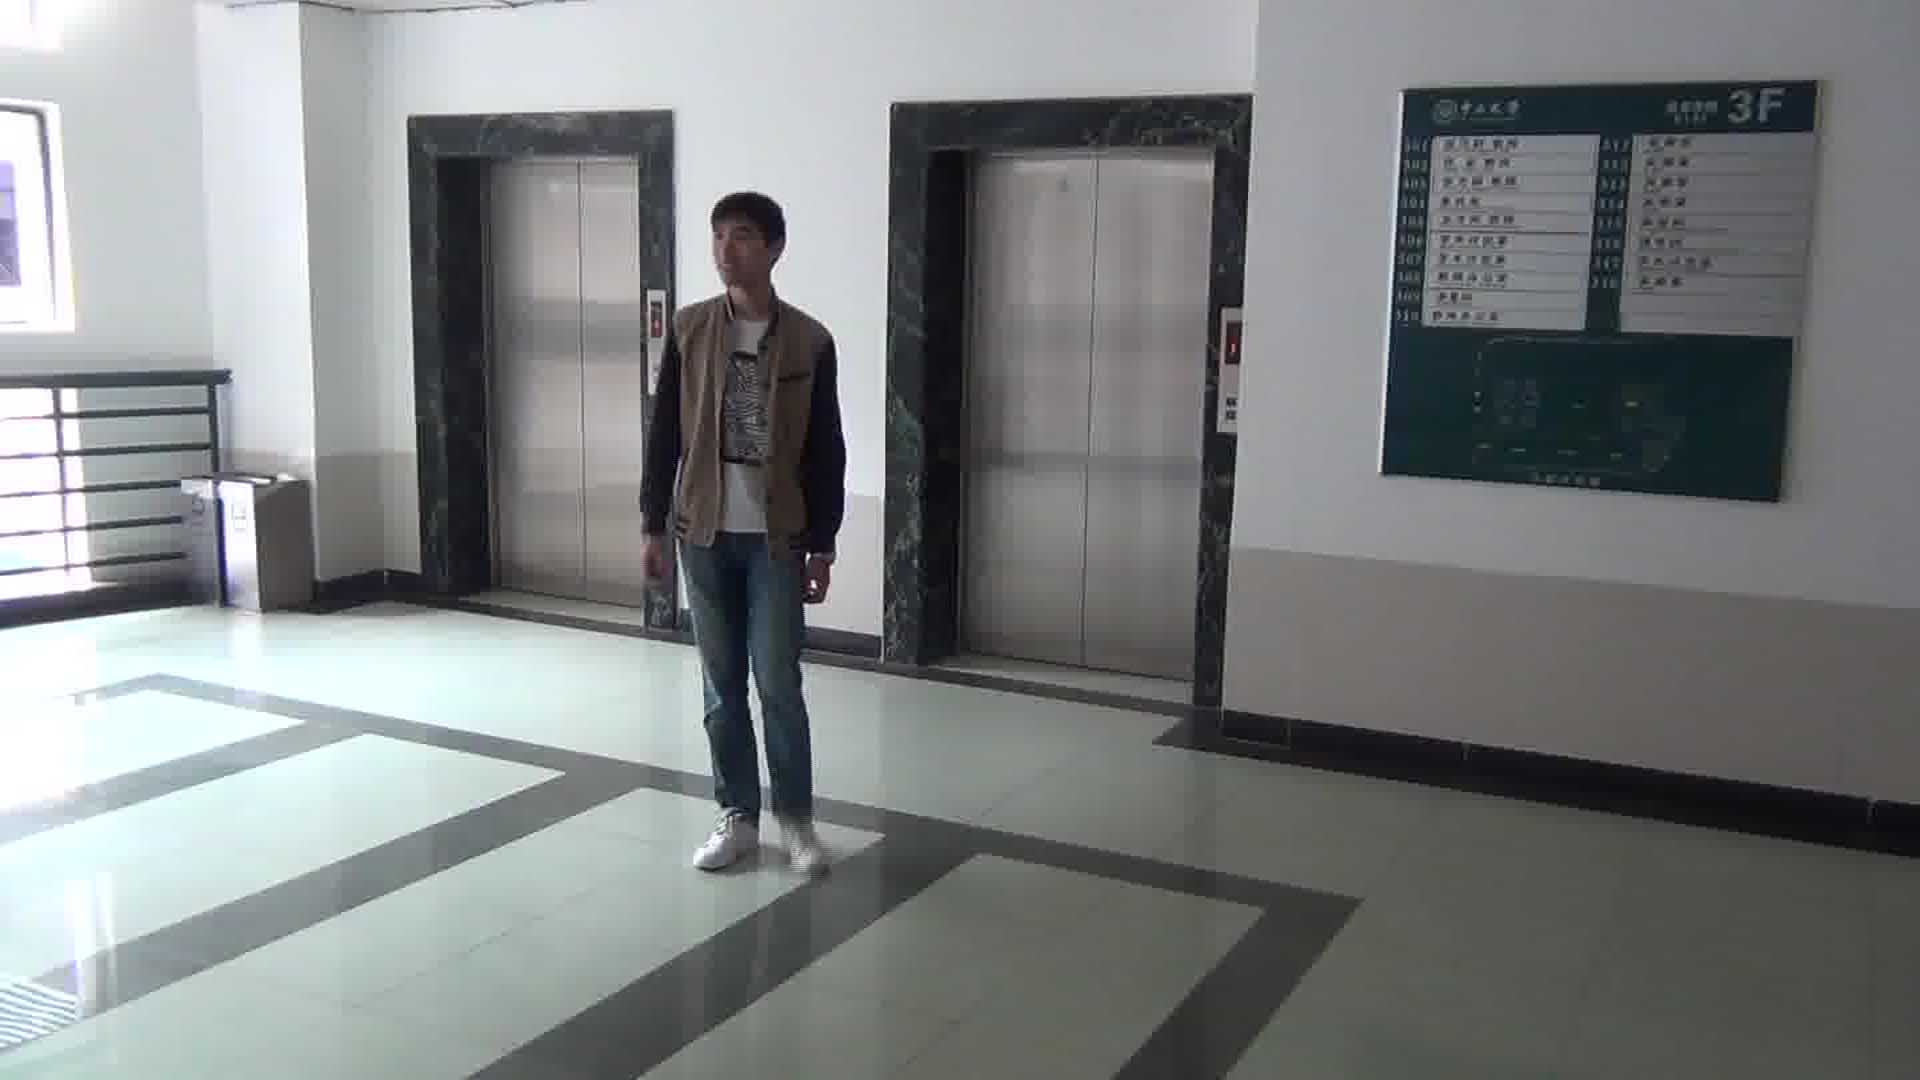
\includegraphics[width=25mm]{3-1}~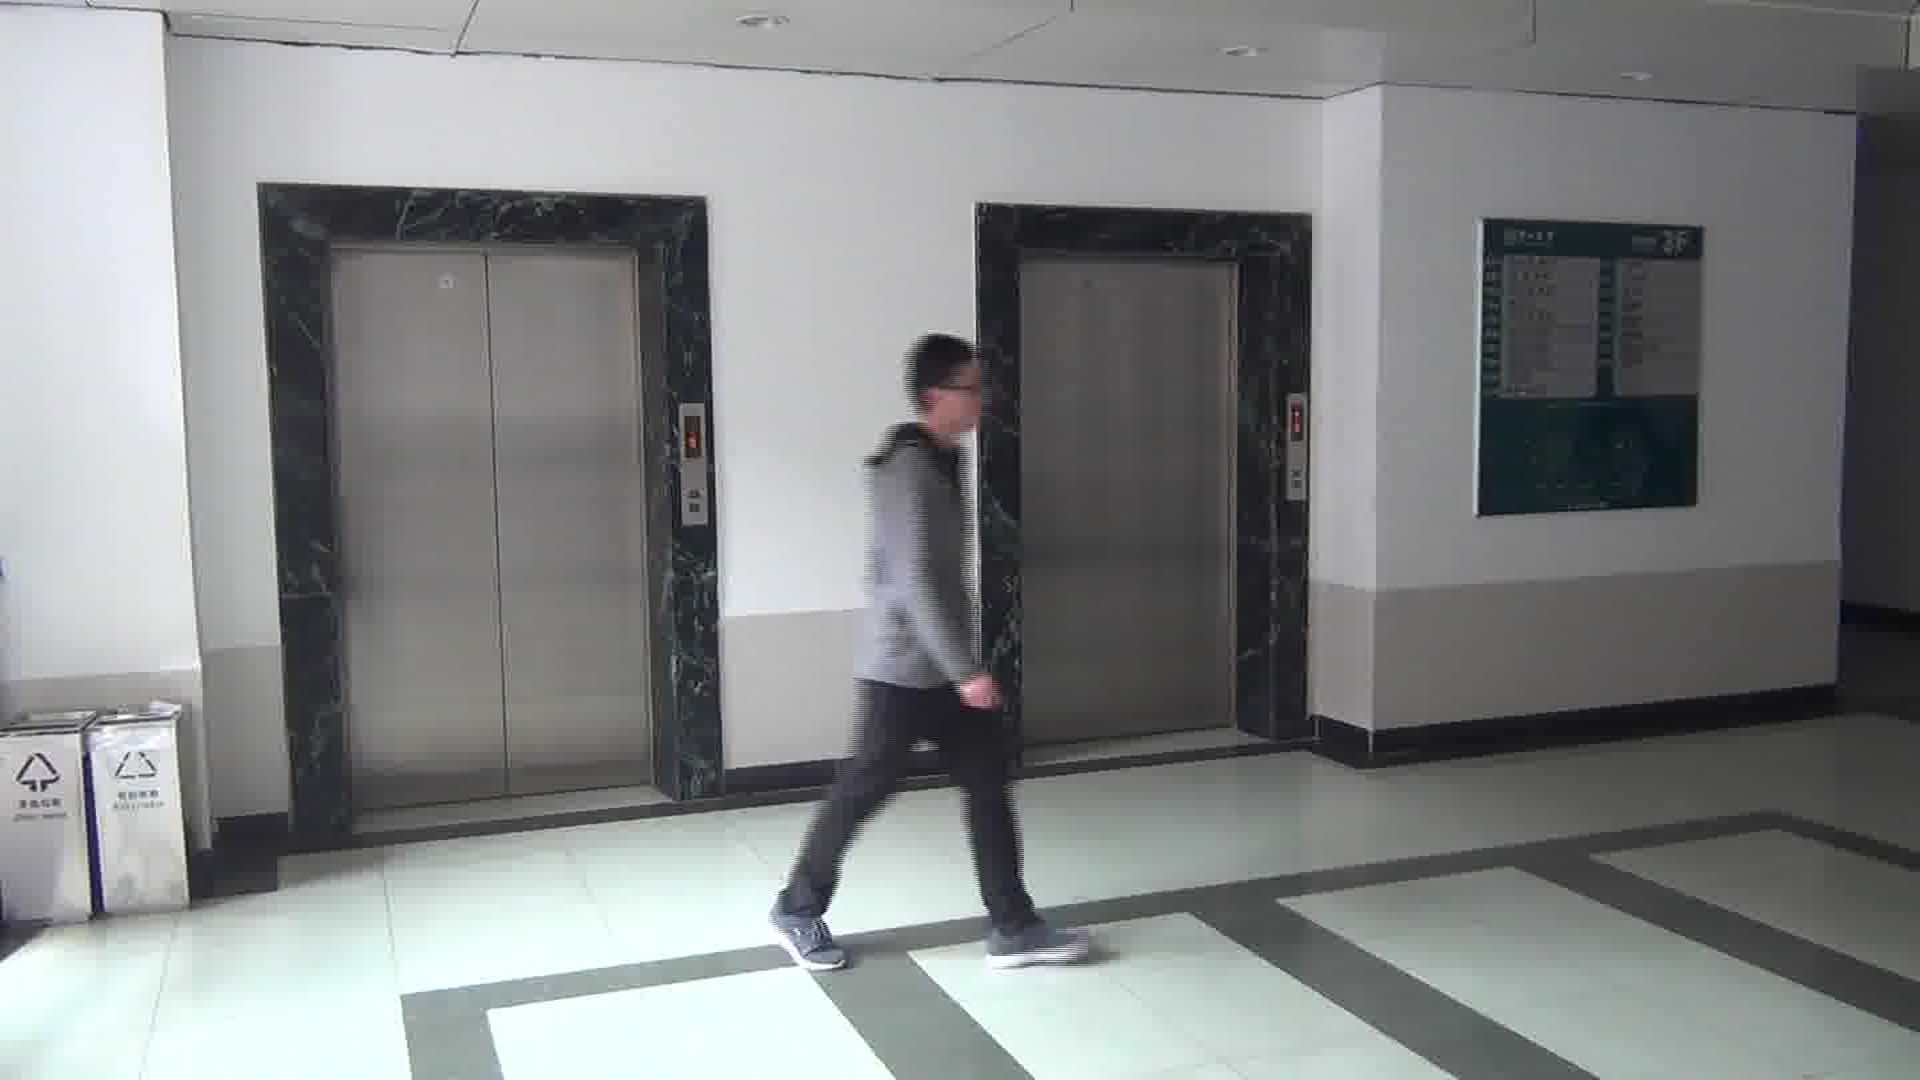
\includegraphics[width=25mm]{3-2}~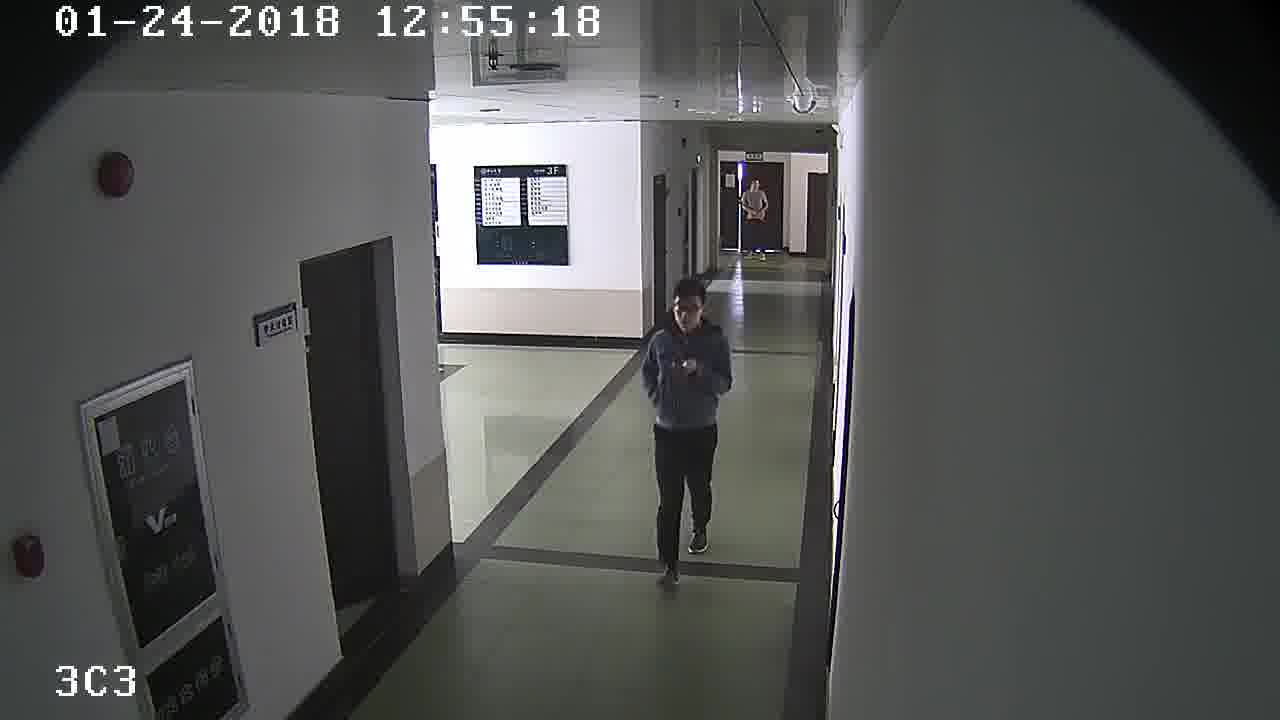
\includegraphics[width=25mm]{3-3} \\
5. 三楼走廊 & 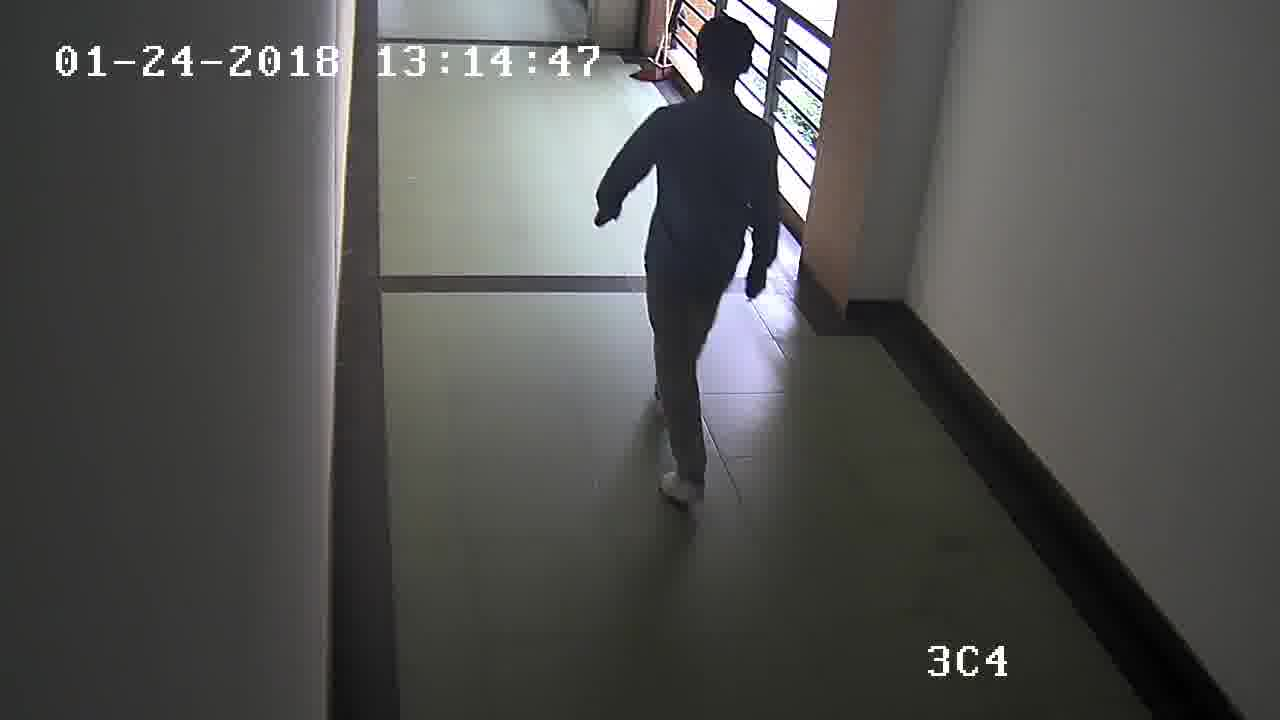
\includegraphics[width=25mm]{3-4}~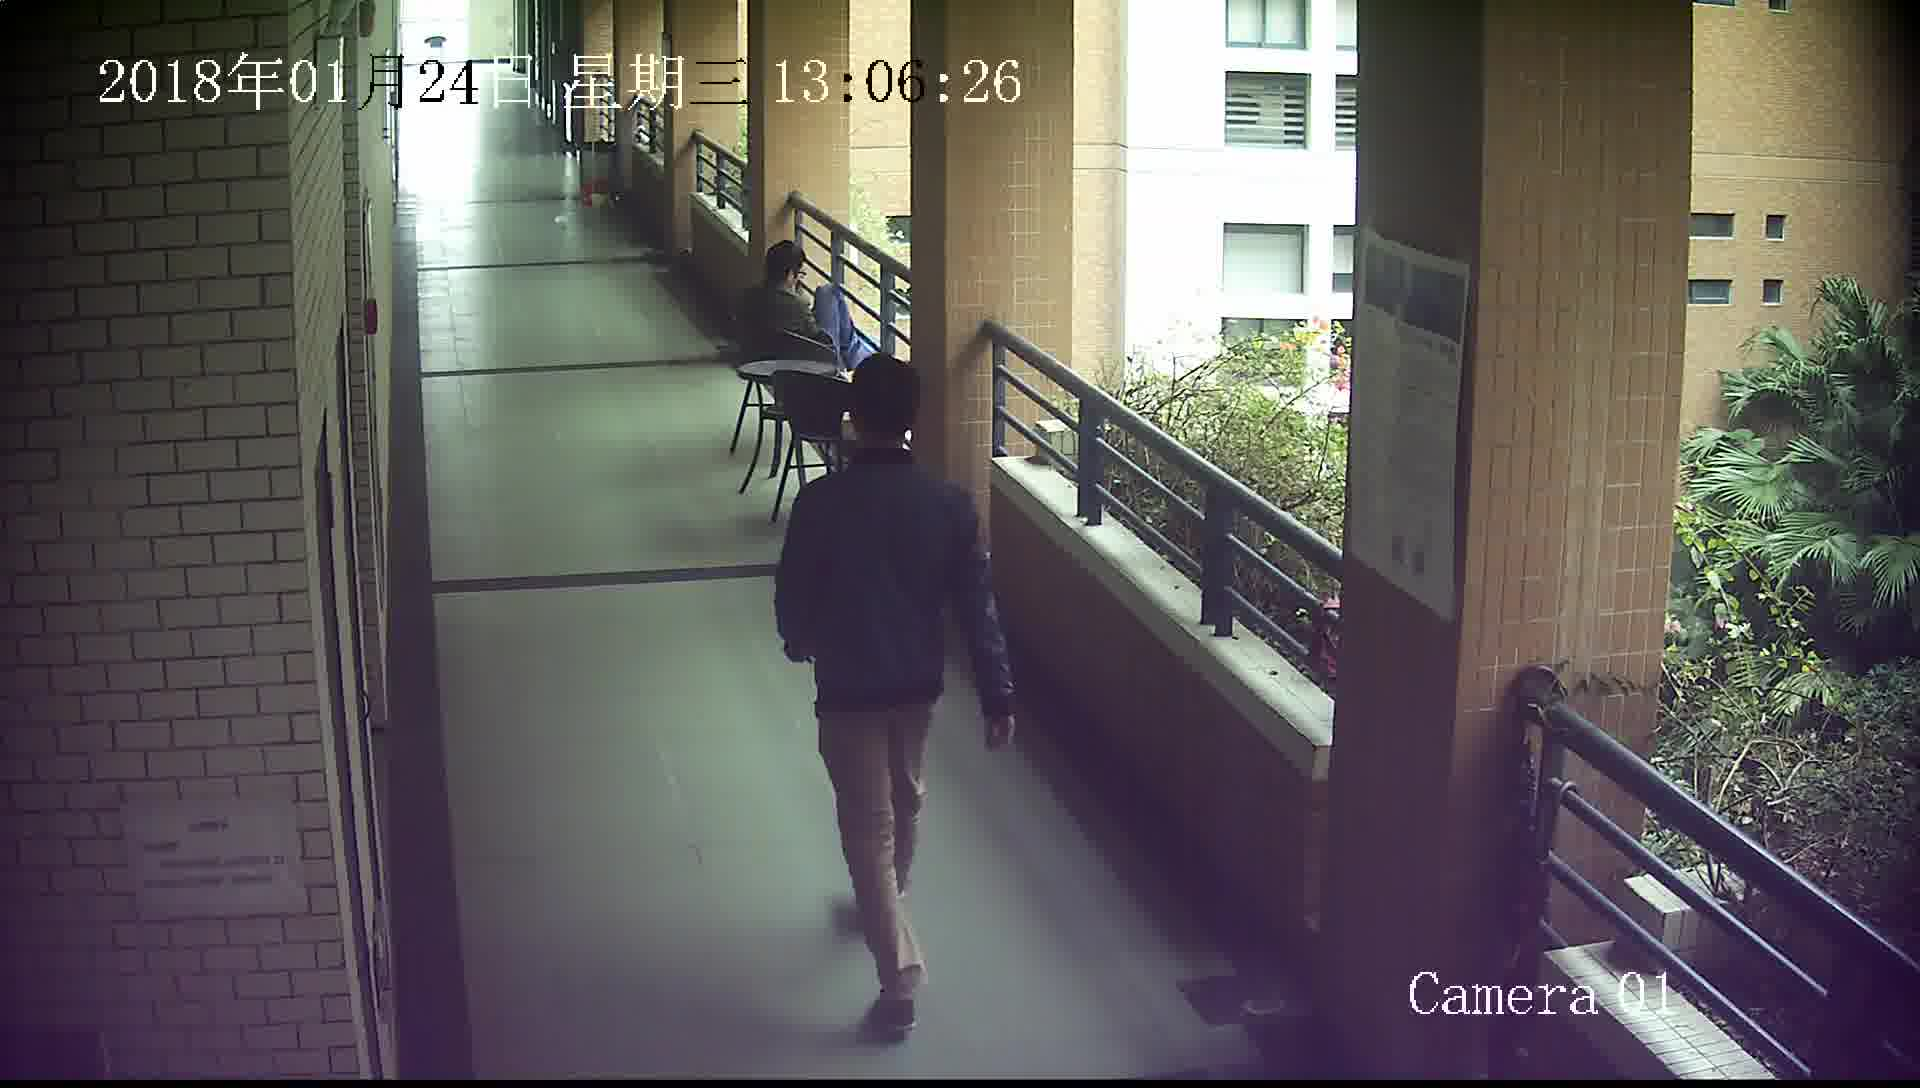
\includegraphics[width=25mm]{3-5}~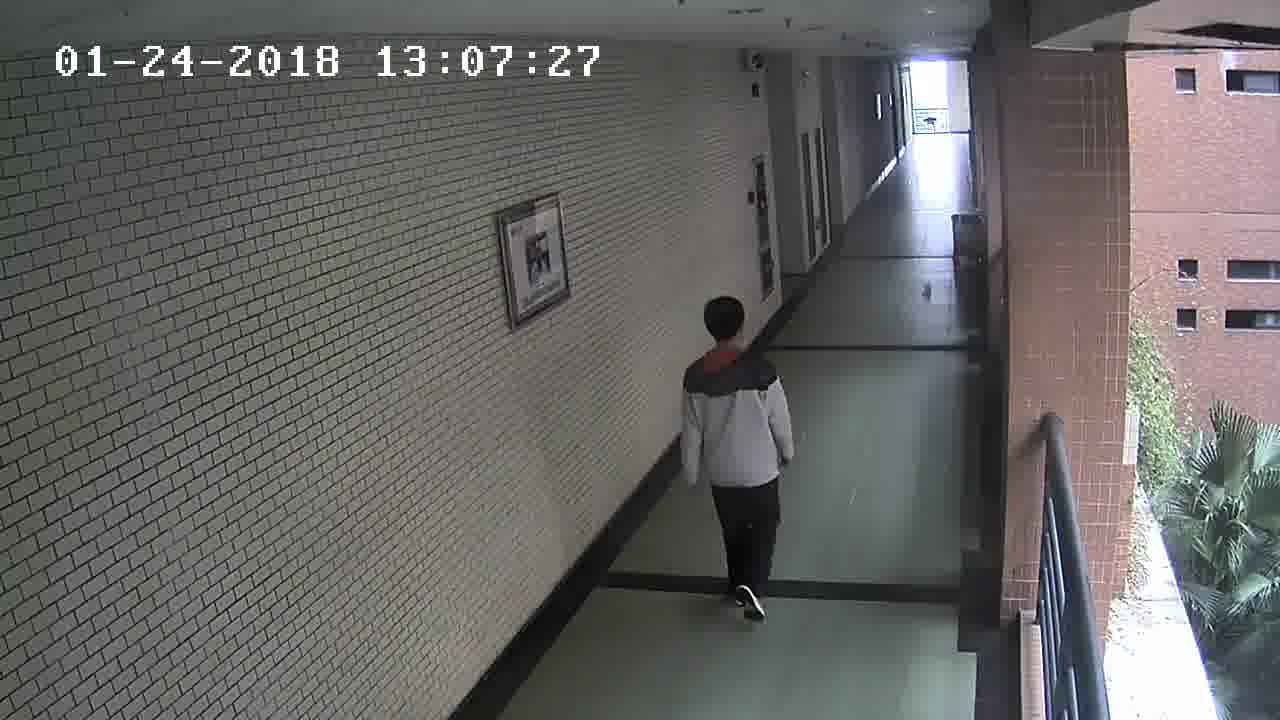
\includegraphics[width=25mm]{3-6}~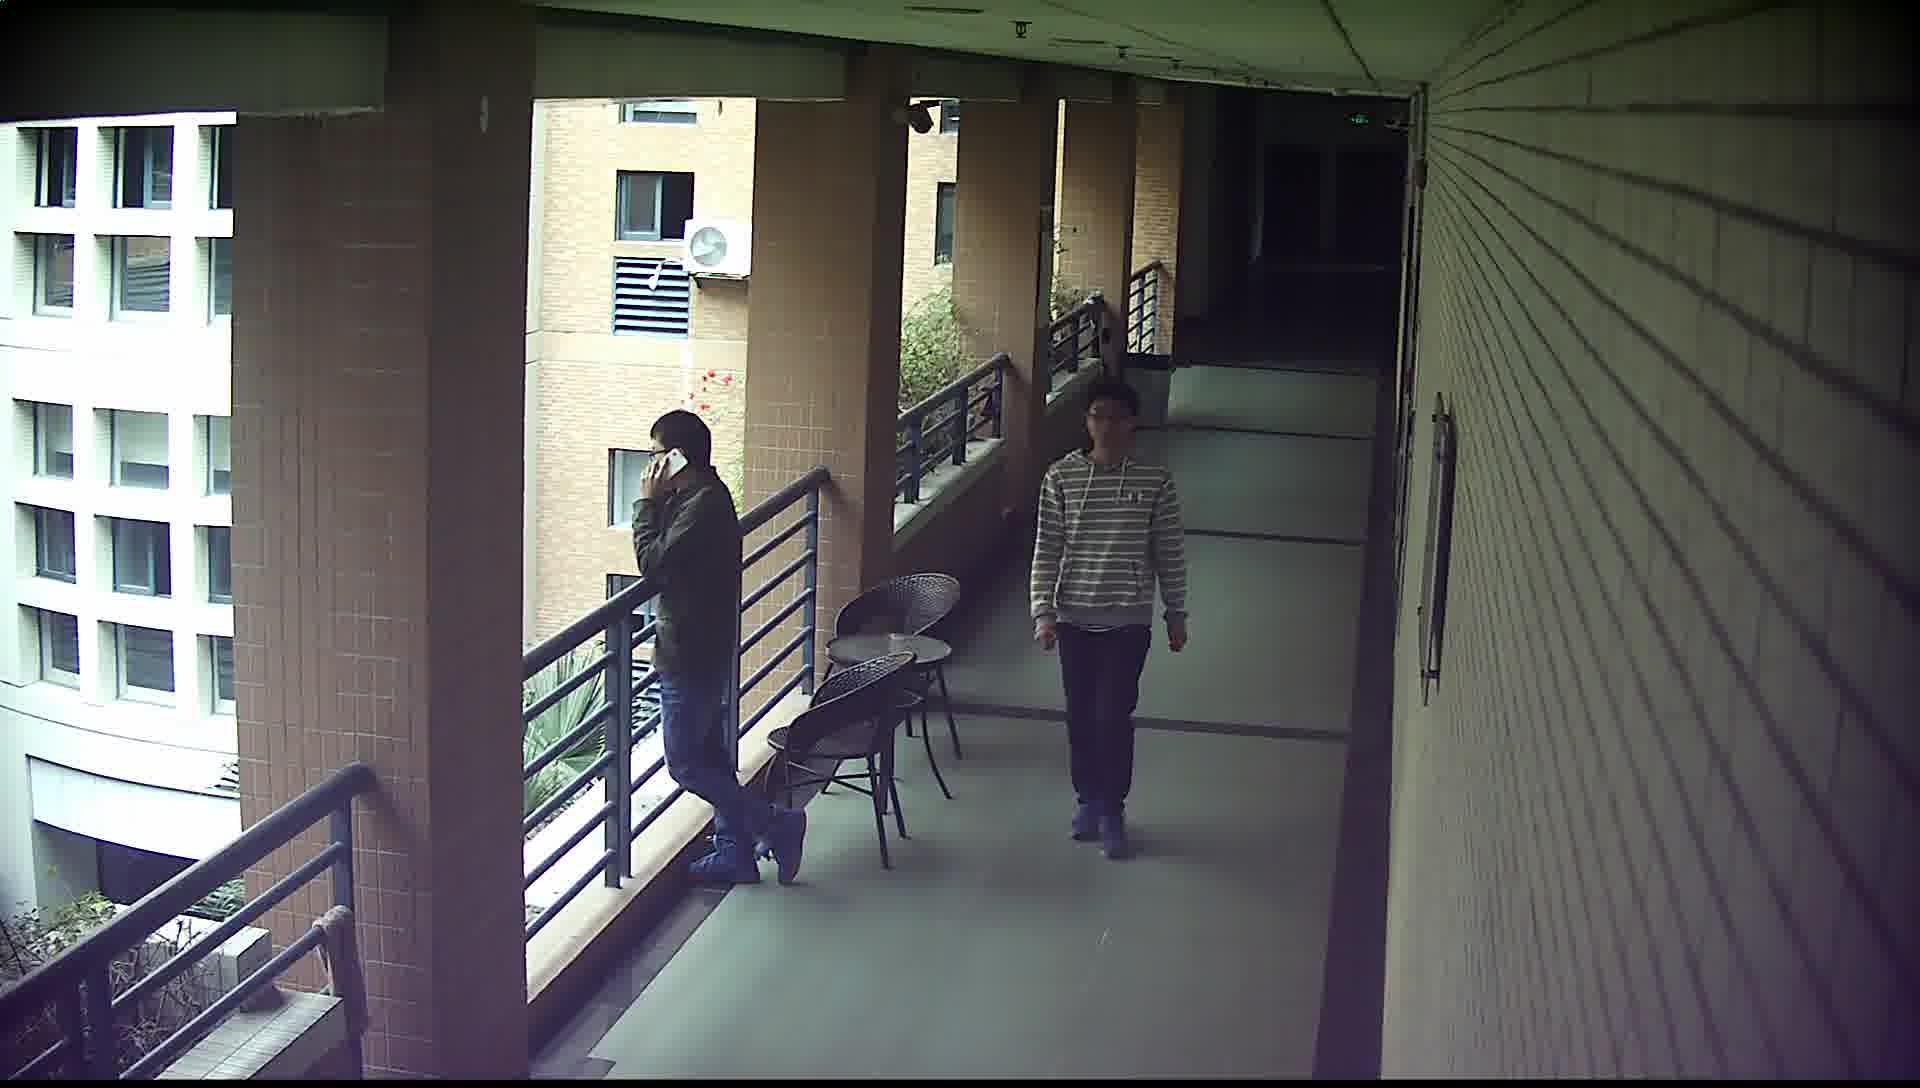
\includegraphics[width=25mm]{3-7} \\
\bottomrule
\end{tabularx}
\end{table}

第5组场景三楼走廊也有类似情况,第1个摄像头的视野很窄,行人能够在很短时间内通过画面,而第4个摄像头则几乎能把行人通过走廊的整个过程记录下来。

\subsection{行人检测效果及人工标注结果}

行人检测使用了Detectron工具,由于Detectron实现了Mask RCNN,所以可以将行人的轮廓分割出来。图\ref{fig:detectron}展示了行人检测可视化的效果。

\begin{figure}[!ht]
\centering
\subfloat[场景1]{\centering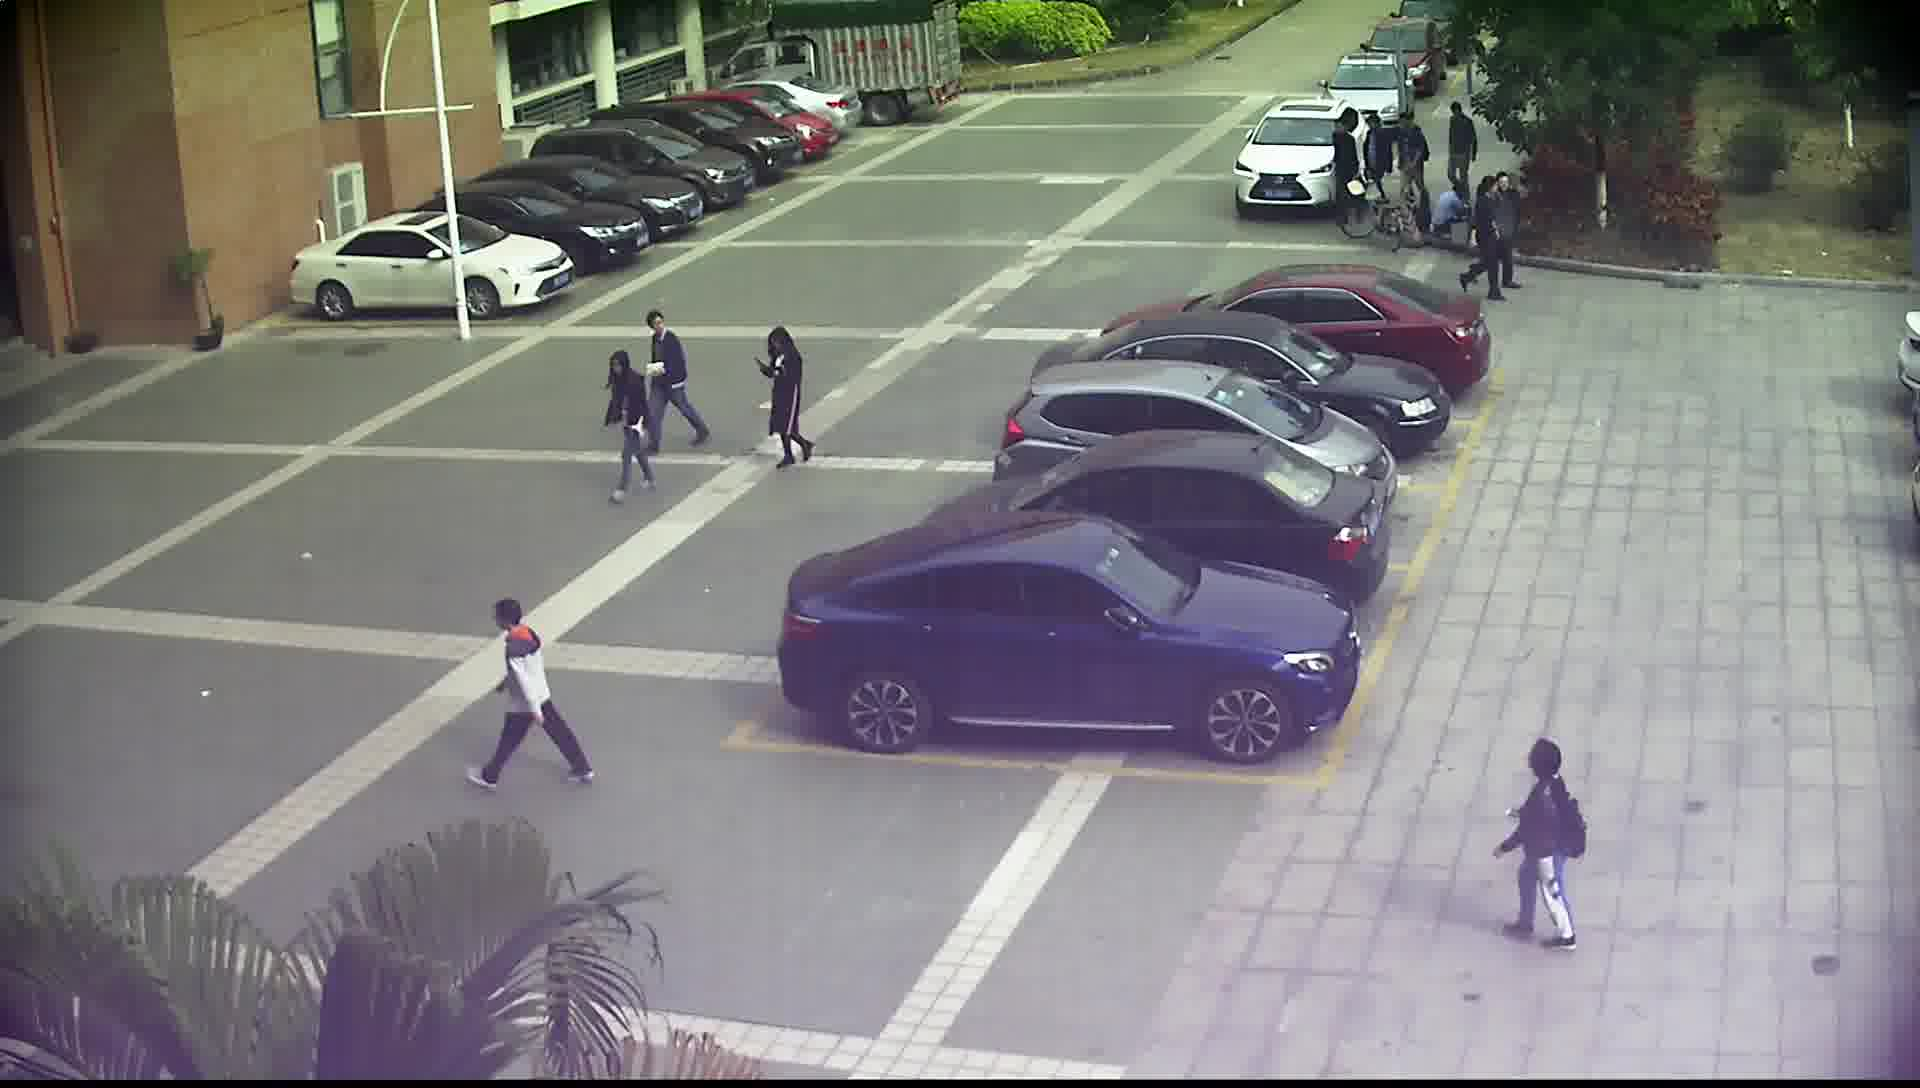
\includegraphics[width=0.4\textwidth]{1-2_5_151}}\quad
\subfloat[场景2]{\centering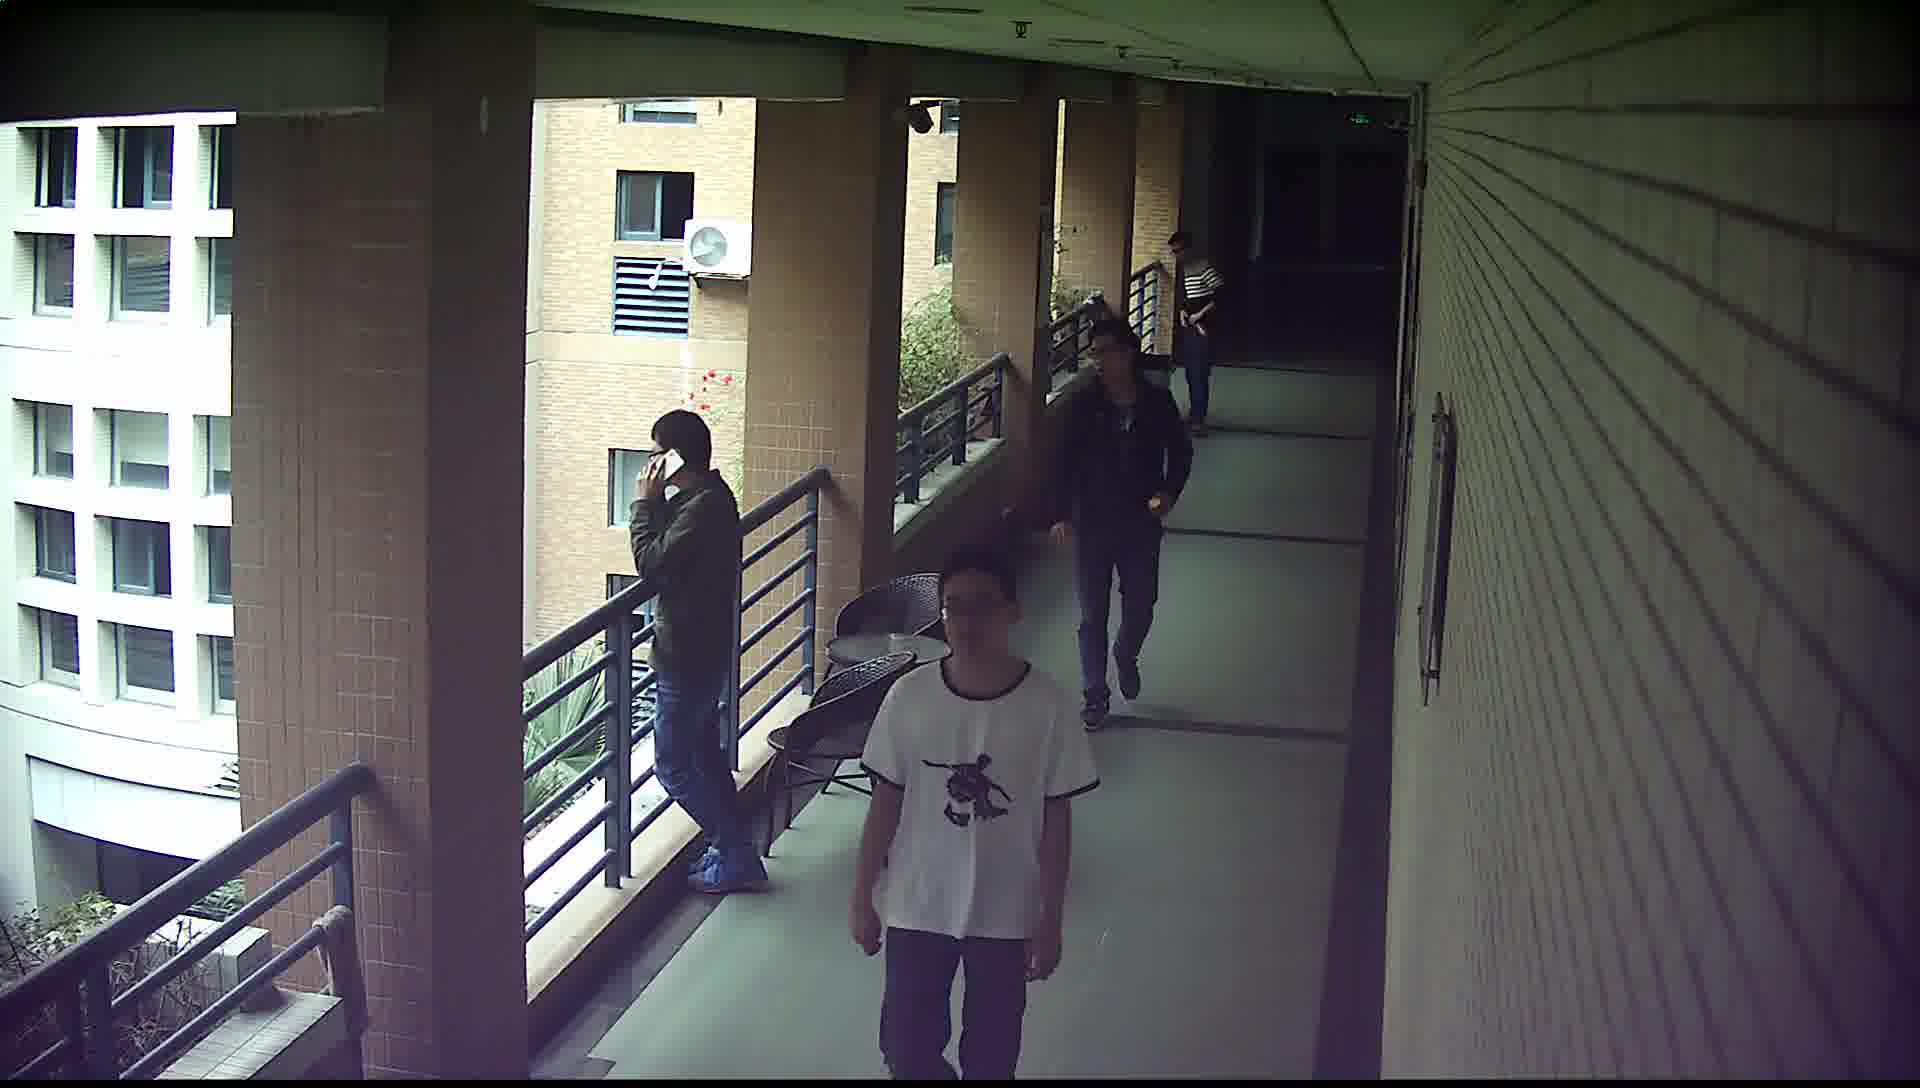
\includegraphics[width=0.4\textwidth]{3-7_10_394}}\\
\subfloat[场景1检测结果]{\centering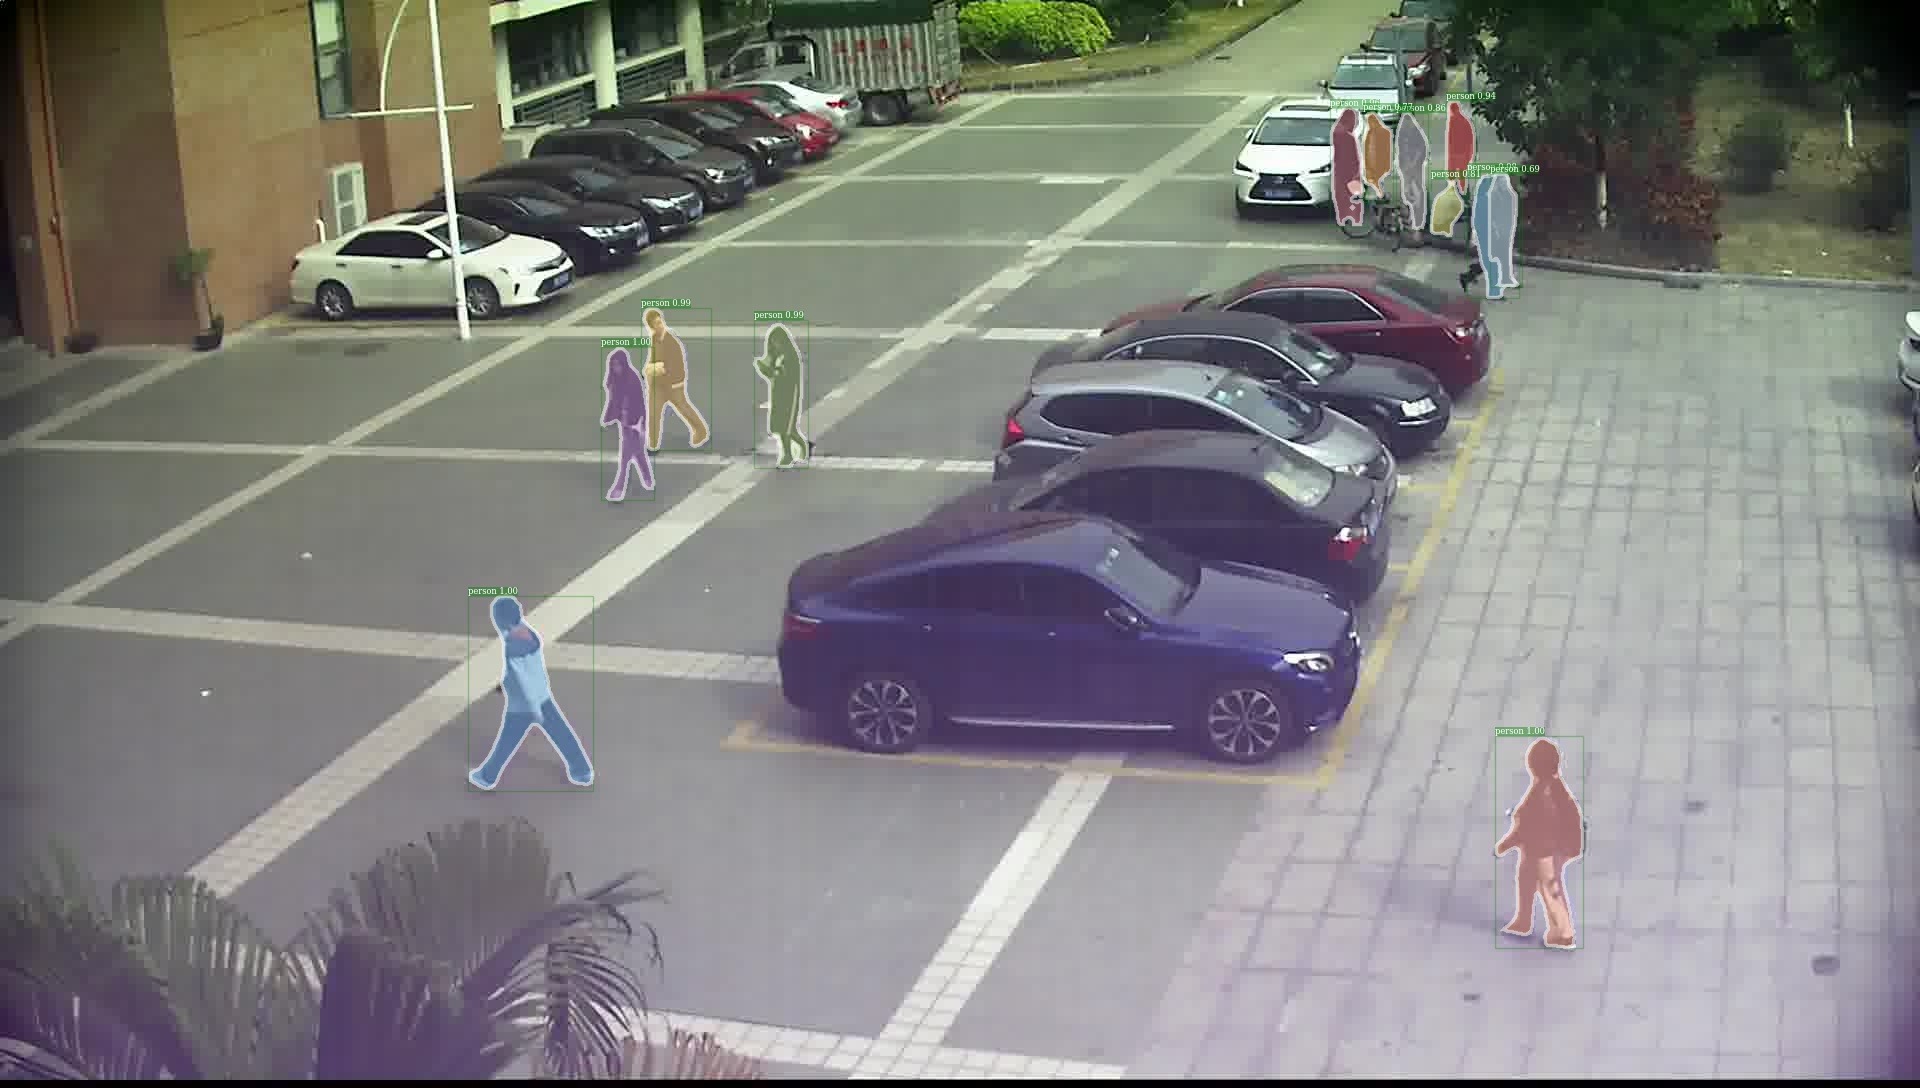
\includegraphics[width=0.4\textwidth]{1-2_5_151_det}}\quad
\subfloat[场景2检测结果]{\centering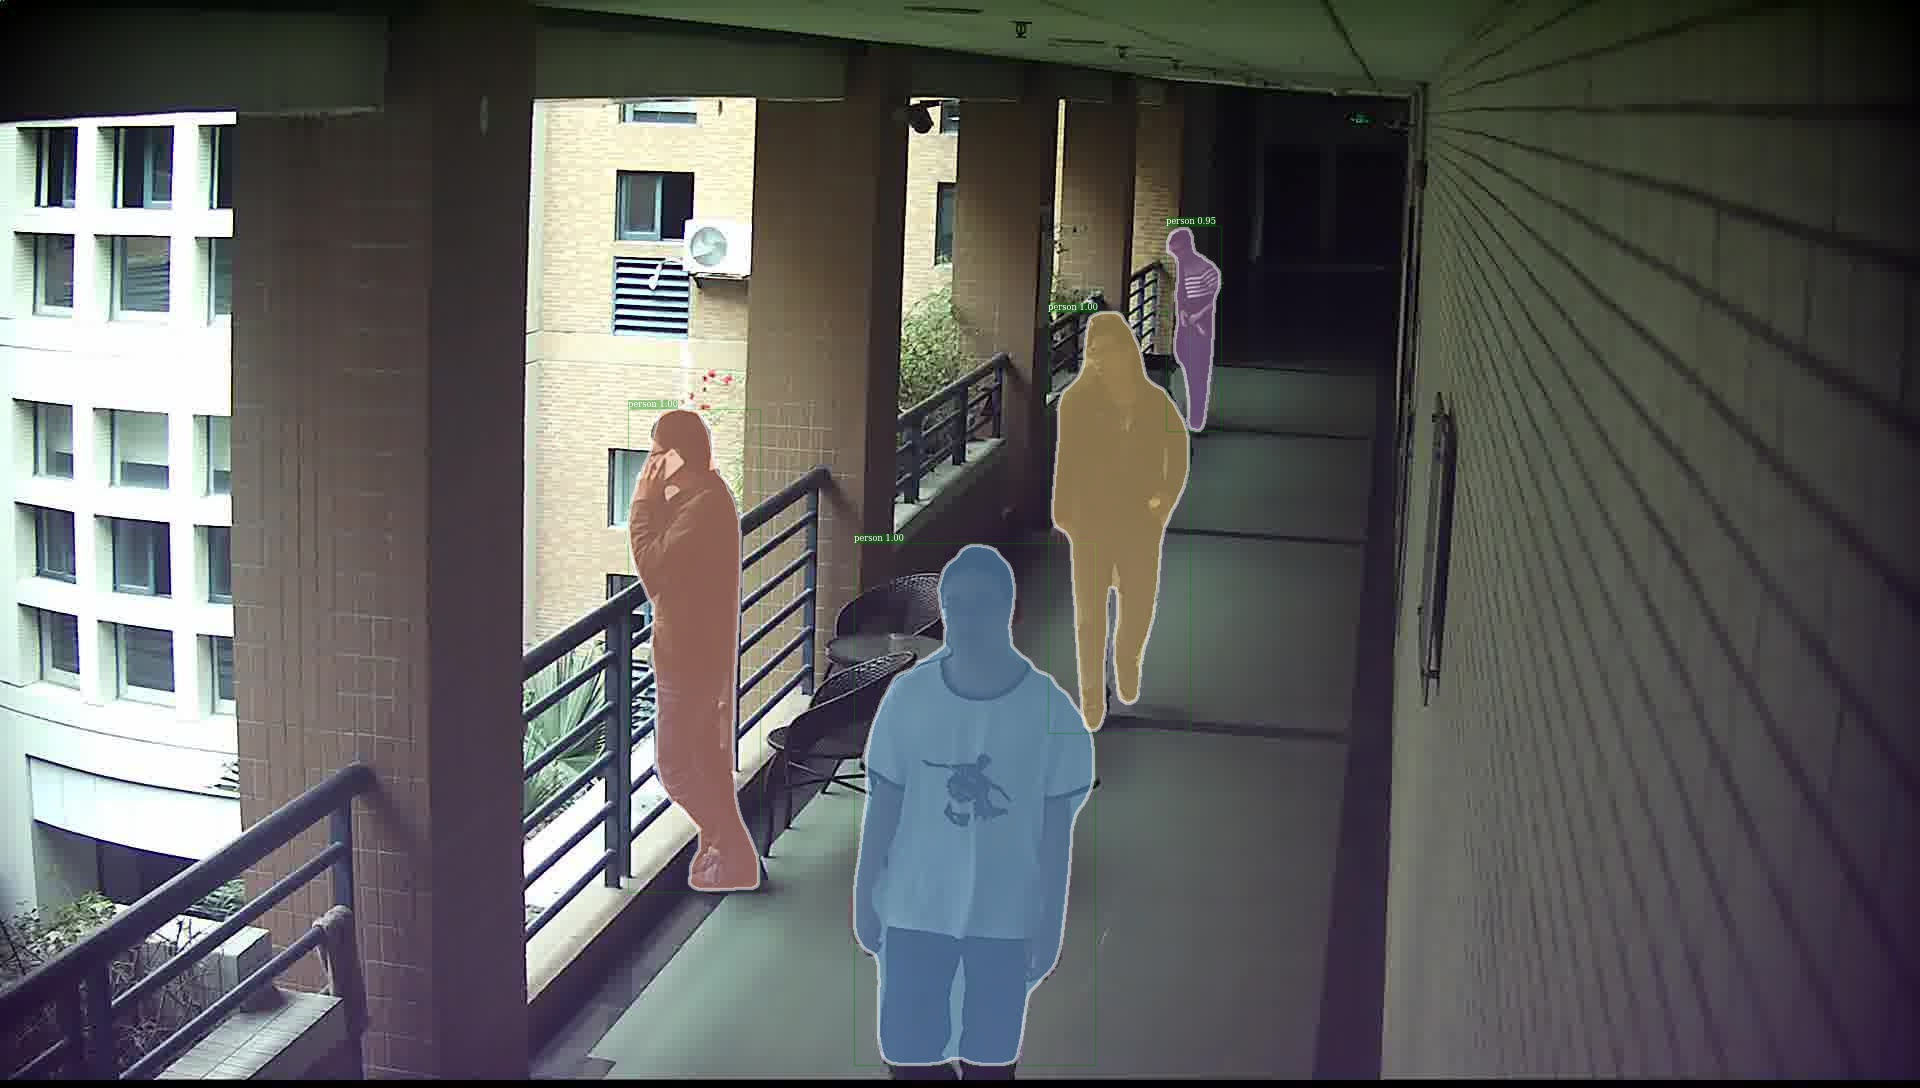
\includegraphics[width=0.4\textwidth]{3-7_10_394_det}}
\caption{Detectron行人检测结果可视化}
\label{fig:detectron}
\end{figure}

图\ref{fig:label}展示了经过人工标注后得到的同一行人在不同摄像头下的图片。从图中可以看出,同一行人在不同的视角下,差距很大,对于行人重识别算法以及人物跟踪任务极具挑战性。

\begin{figure}[!ht]
\centering
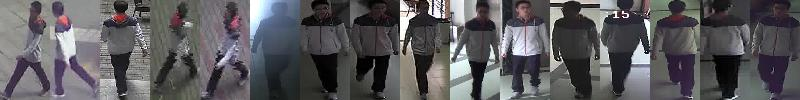
\includegraphics[width=\textwidth]{label}
\caption{同一行人在不同摄像头下的图片}
\label{fig:label}
\end{figure}\vspace{-1em}

\section{行人重识别算法}

\subsection{训练Loss曲线}

训练阶段交叉熵误差(Loss)随着数据集训练批次数(Epoch)变化曲线如图\ref{fig:loss}所示。图中共展示了第\ref{sec:modeltraining}小节所述的3个训练阶段的训练过程,每个阶段包含60个Epoch。从图中可以看出,交叉熵误差在第一训练阶段下降很明显,同时之后的测试结果\cite{sun2017beyond}也显示只使用基线模型也能达到较好的效果,说明了基线模型的稳健性。

\begin{figure}[!ht]
\centering
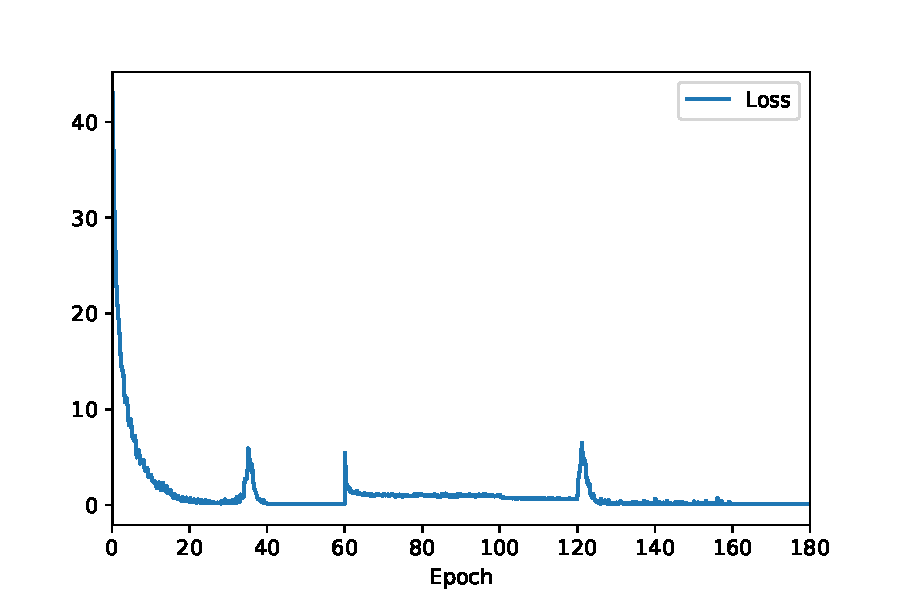
\includegraphics[width=0.6\textwidth]{loss}
\caption{交叉熵误差随着迭代次数变化曲线}
\label{fig:loss}
\end{figure}

\subsection{测试准确率比较}

表\ref{tab:test}为在Market1501测试集上的测试结果,可以看出复现的结果接近达到原论文\cite{sun2017beyond}中显示的结果。从表中可以看出,我们的PCB模型的结果以及很接近原论文中所显示的结果,但存在一个问题,我们的模型中使用RPP方法带来的提升,不及其在原论文中的表现,说明我们RPP方法的实现存在与原论文不符的情况。由于原作者尚未公布源代码,所以只能推测导致这些差异可能存在的原因:一、模型参数的初始化方式不一致,导致我们的模型与原论文中的模型收敛到了不同的局部最小值;二、不确定原始RPP模型中用于像素分类的神经网络层是否加入了Batch Normalization\cite{ioffe2015batch}层和Dropout\cite{srivastava2014dropout}层,以及它们的具体参数是多少;三、训练过程不一致,在原论文中没有清晰地说明三个训练阶段的Epoch数,以及每个训练阶段的学习率变化情况,所以只能靠人工调参。

\begin{table}[!ht]
    \centering
    \caption{Market1501数据集测试结果}
    \label{tab:test}
    \begin{threeparttable}
    \begin{tabularx}{\textwidth}{p{0.28\textwidth}p{0.2\textwidth}<{\centering}p{0.2\textwidth}<{\centering}p{0.2\textwidth}<{\centering}}
    \toprule
                            & mAP~(\%)   & Rank1~(\%) & Rank10~(\%) \\ \midrule
    PCB~(paper)~\tnote{a}    & 77.40  & 92.30  & 98.20   \\
    PCB+RPP~(paper)~\tnote{a}& 81.60  & 93.80  & 98.50   \\
    PCB                      & 73.10  & 87.20  & 93.40   \\
    PCB+RPP                  & 74.03  & 89.43  & 94.40   \\ \bottomrule
    \end{tabularx}
    \begin{tablenotes}
        \footnotesize
        \item[a] 原论文\cite{sun2017beyond}中显示的结果。
    \end{tablenotes}
    \end{threeparttable}

\end{table}

\subsection{测试结果可视化}

图\ref{fig:testvis}是行人重识别模型在Market1501数据集上测试结果的可视化,左边一列是查询图片,每一张查询图片相应的右边一行是从测试库中挑选出来的图片,有红色边框的图片代表该人物标签与相应的查询图片人物标签不一致。从图中可以看出模型的效果比较理想,仅存在少量出错的情况。同时注意到原数据库\cite{zheng2015scalable}中存在ground truth出错的情况,影响了评估指标的准确性。

\begin{figure}[!ht]
    \centering
    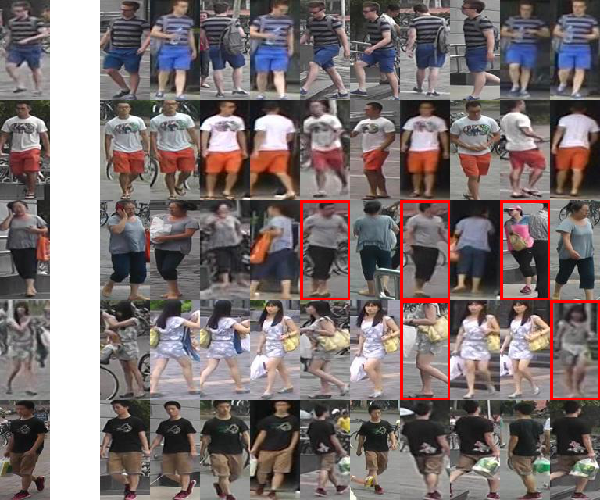
\includegraphics[width=0.7\textwidth]{vis3}
    \caption{测试结果可视化}
    \label{fig:testvis}
\end{figure}

\section{强化学习算法}

\subsection{学习后选择的部署方案}

表\ref{tab:rlresult}为经过强化学习训练后的智能体在应对各种状态时,最有可能采取的行动统计。其中方案~(1, 2, 7, 10, 14)~表示摄像头ID分别为1, 2, 7, 10, 14的部署方案,其它方案的表示可以此类推。表中第二列表示该方案作为其它方案的最优转移方案的频次,第三列表示该方案最优频次占方案总数的比例。

智能体经过强化学习训练,对当前环境有了了解之后,假设采用贪心的策略,即无论当前处于什么状态,都采取使得长期价值最高的动作。基于此假设,表\ref{tab:rlresult}显示,在所有可能的状态中,智能体处于其中的约$2/3$的状态下时都会一次性地转入~(1, 2, 7, 10, 14)~状态,因此该状态可以认为是智能体所选择的最优状态,该状态的可视化结果见图\ref{fig:rlresult}。处于其余约$1/3$的状态下时会转入~(1, 2, 7, 10, 13)~这个次优状态,可以看出,此方案与最优方案之间的区别,仅仅在于最后一组的摄像头的选择,而经过检查,该摄像头的成像质量也比较优秀。与此同时,当智能体处于该次优方案的状态时,长期价值最高的动作是转入最优方案状态。同时剩余的三种状态也会马上转入最优方案状态。因此可以得出结论:无论智能体当前处于什么状态,至多经过两步,即可到达最优状态。

\begin{table}[h!]
    \centering
    \caption{学习后选择的部署方案}
    \label{tab:rlresult}
    \begin{tabularx}{\textwidth}{p{0.4\textwidth}p{0.3\textwidth}p{0.3\textwidth}}
    \toprule
    方案               & 频次  & 占比~(\%)  \\ \midrule
    (1, 2, 7, 10, 14) & 190 & 65.97 \\
    (1, 2, 7, 10, 13) & 78  & 27.08 \\
    (1, 2, 7, 9, 14)  & 18  & 6.15  \\
    (1, 3, 7, 10, 14) & 1   & 0.35  \\
    (0, 2, 7, 10, 14) & 1   & 0.35  \\ \bottomrule
    \end{tabularx}
\end{table}

图\ref{fig:rlresult}是监控方案(1, 2, 7, 10, 14)的可视化结果。图中的每一张图片代表从一组摄像头中选取的一个摄像头所拍摄的场景。从图中可以看到,选取的摄像头光线充足、画面清晰、角度端正、视野范围宽阔,是一个理想的摄像头部署方案。

\begin{figure}[!ht]
    \centering
    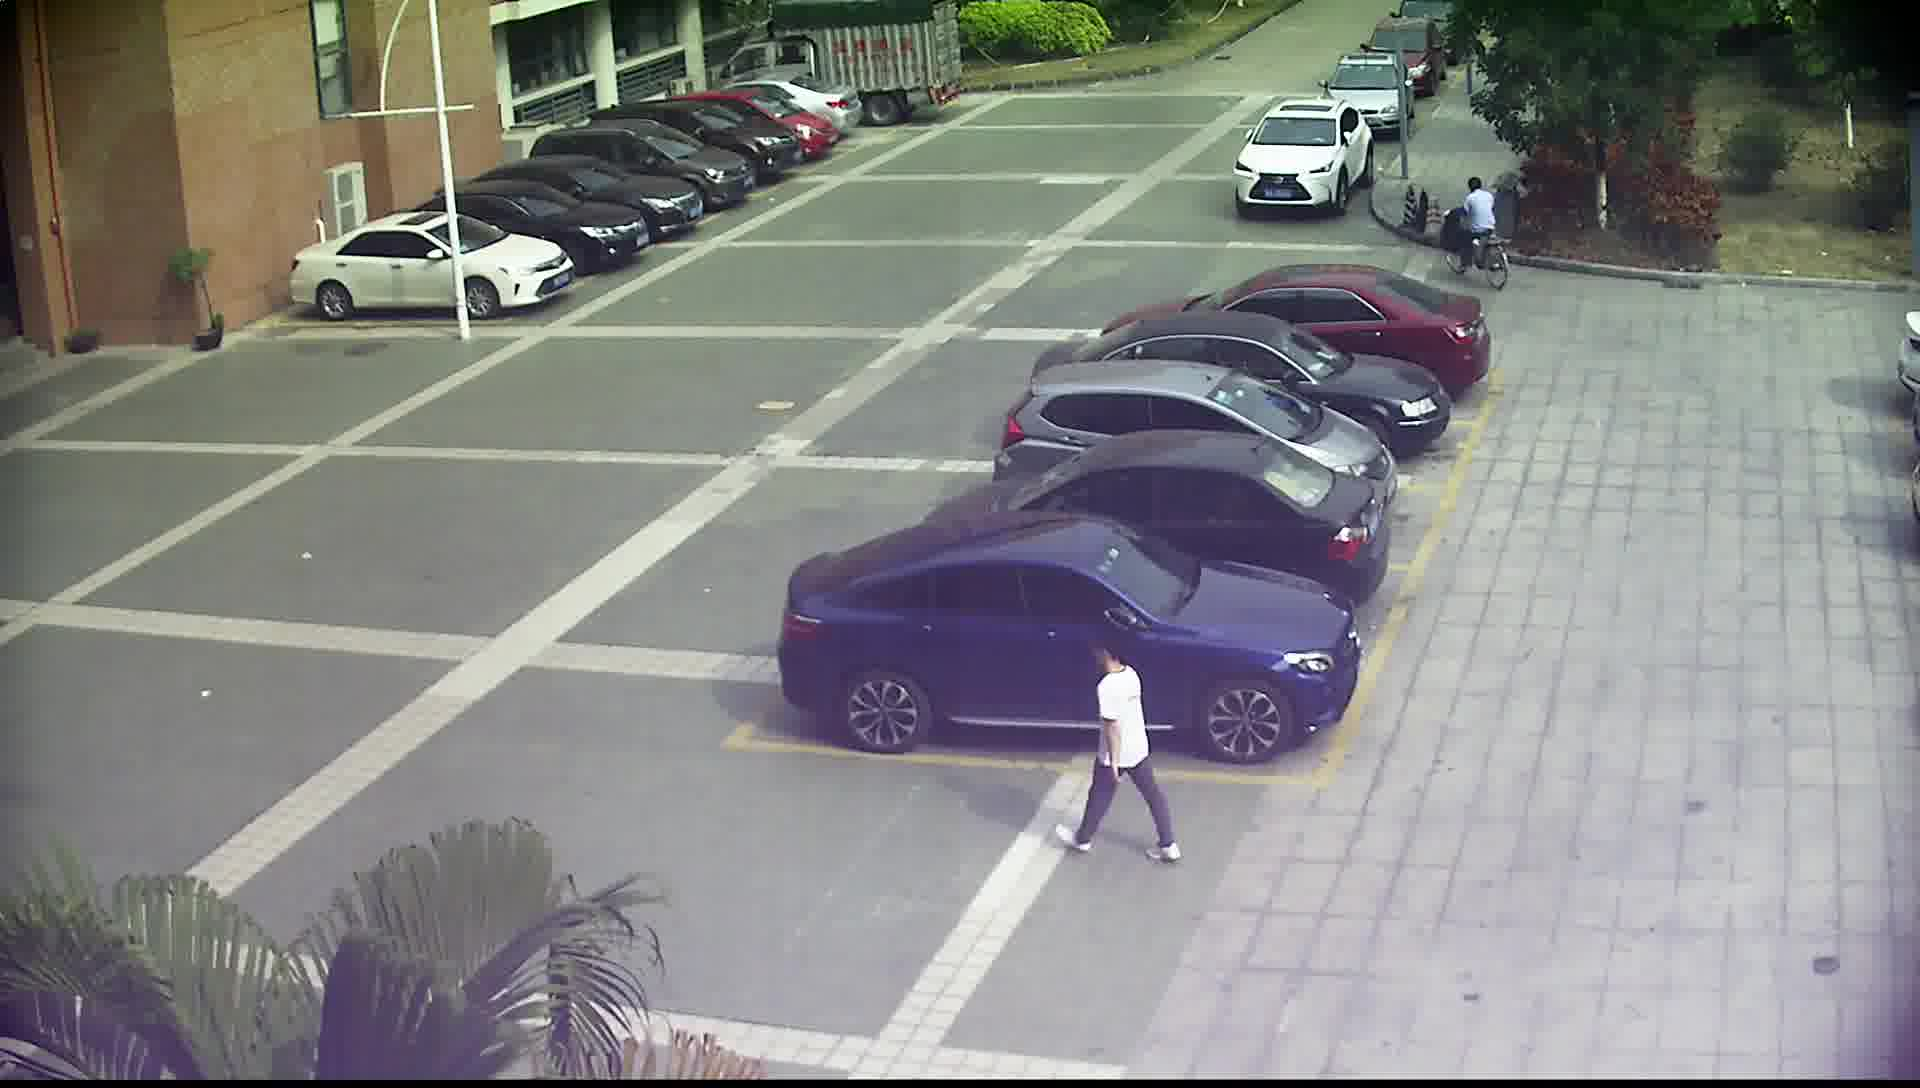
\includegraphics[width=0.3\textwidth]{1-2}
    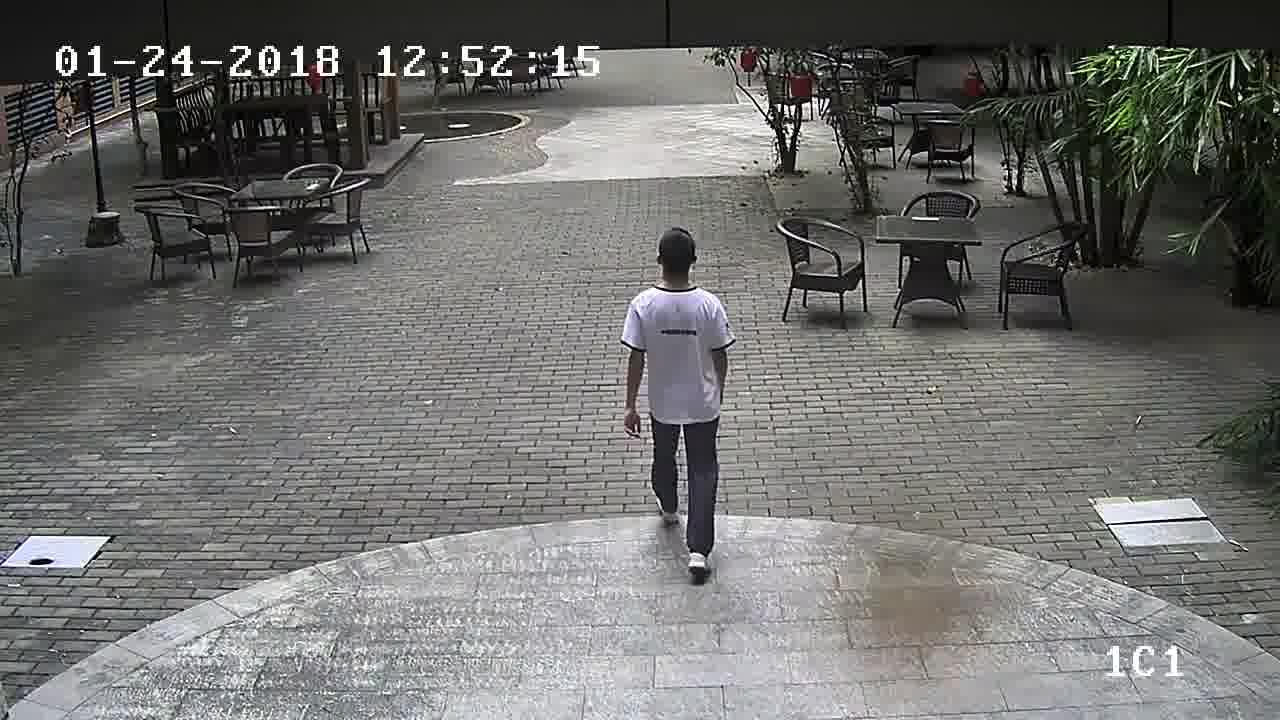
\includegraphics[width=0.3\textwidth]{1-4}\\
    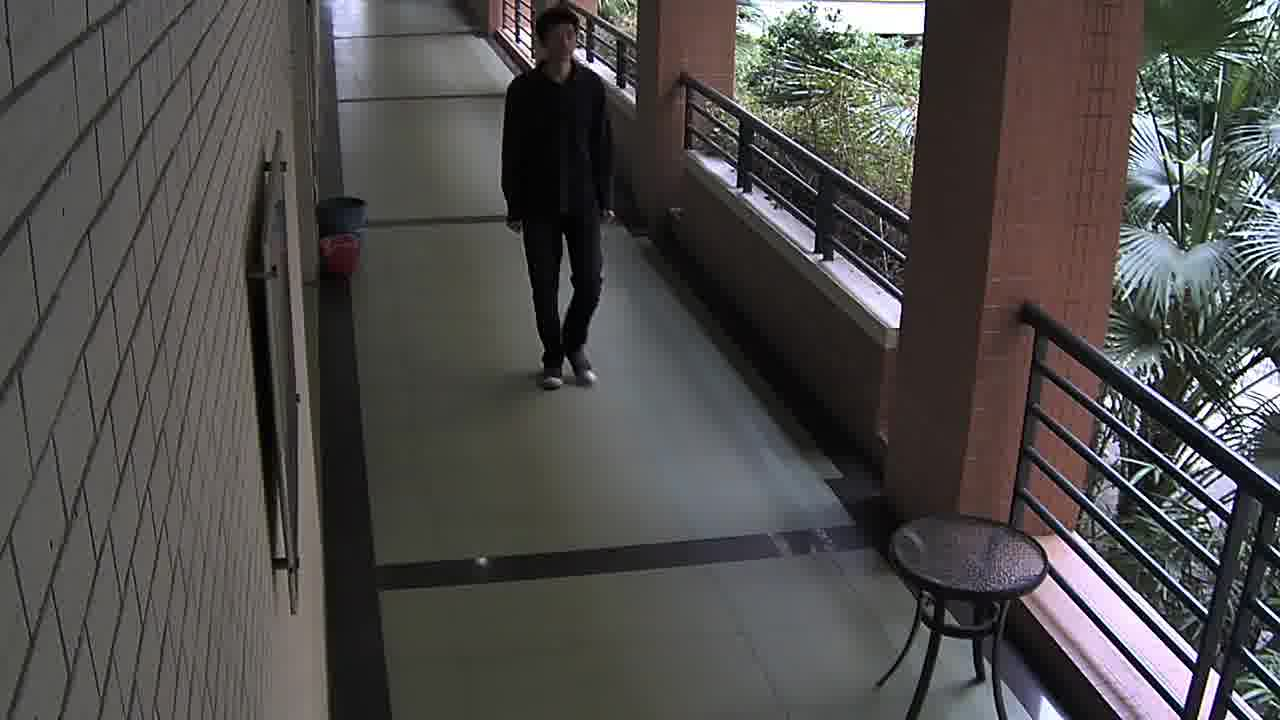
\includegraphics[width=0.3\textwidth]{2-3}
    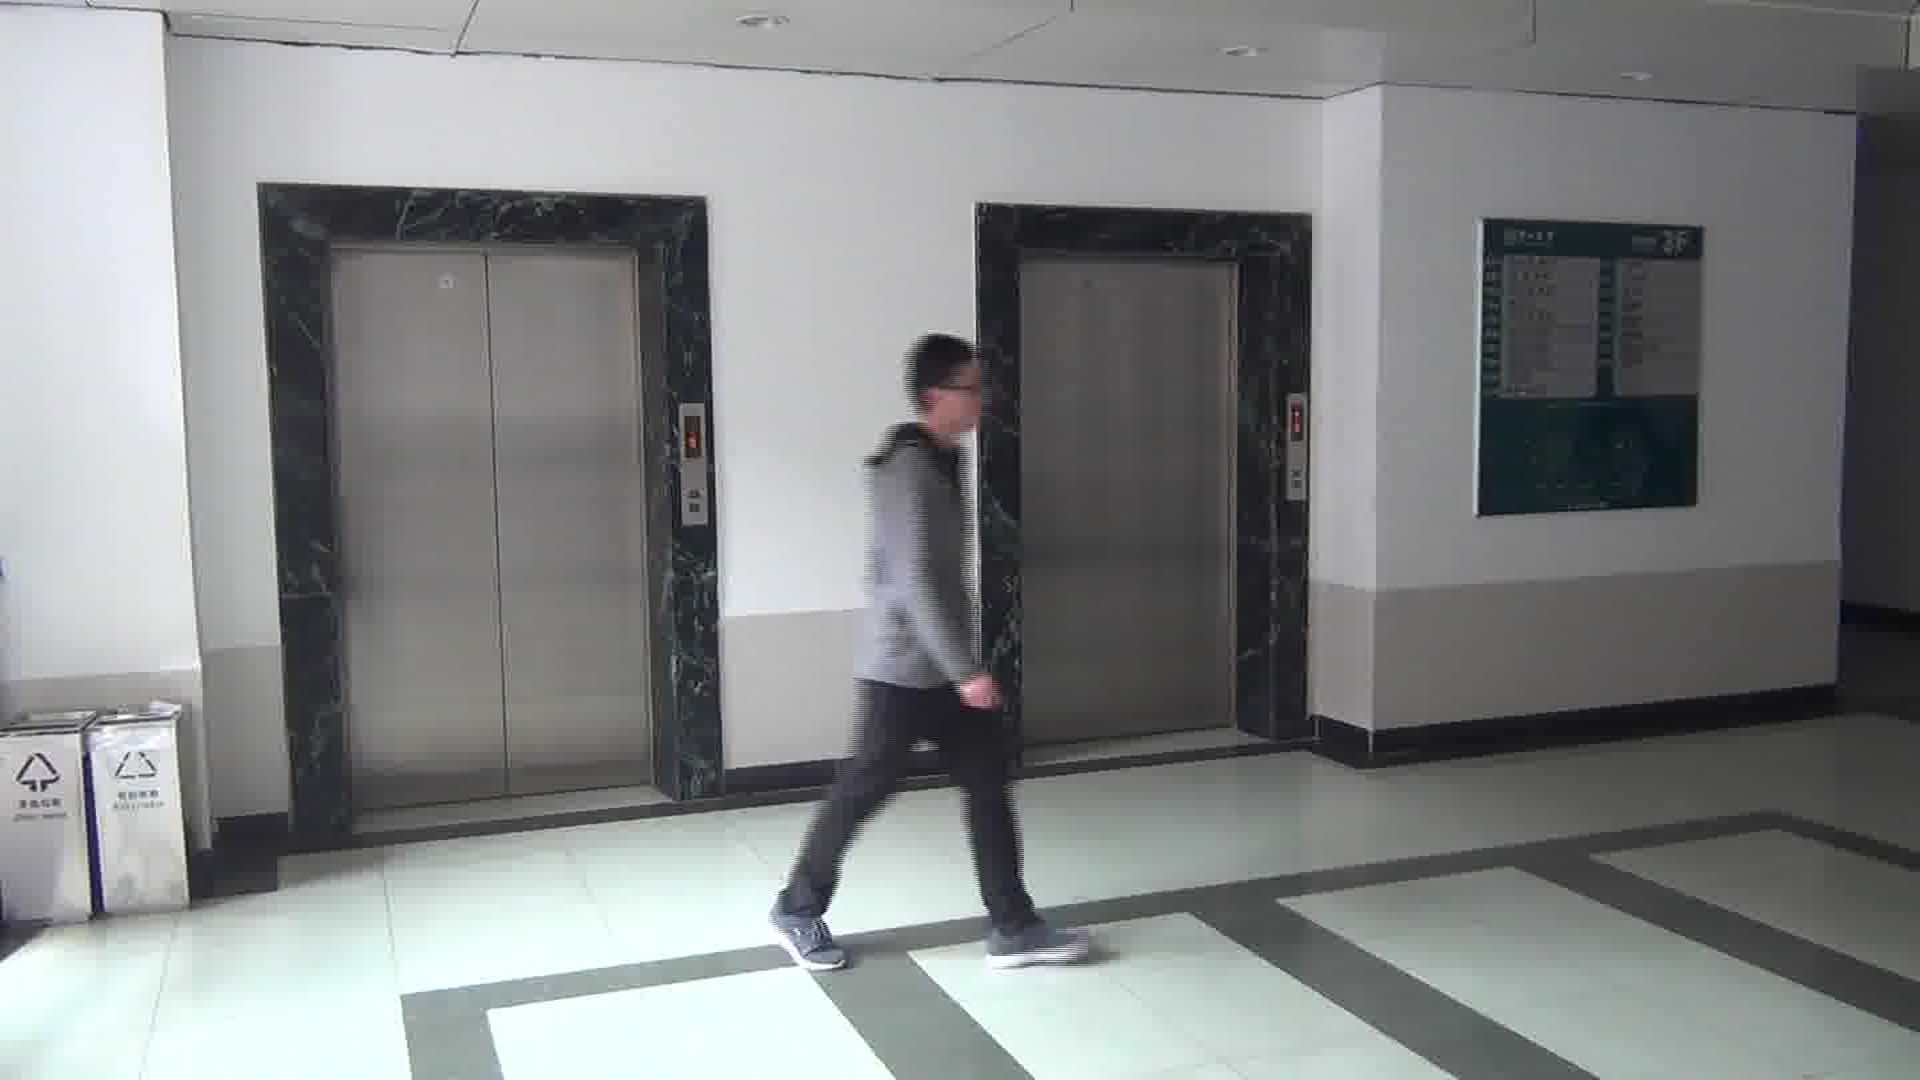
\includegraphics[width=0.3\textwidth]{3-2}
    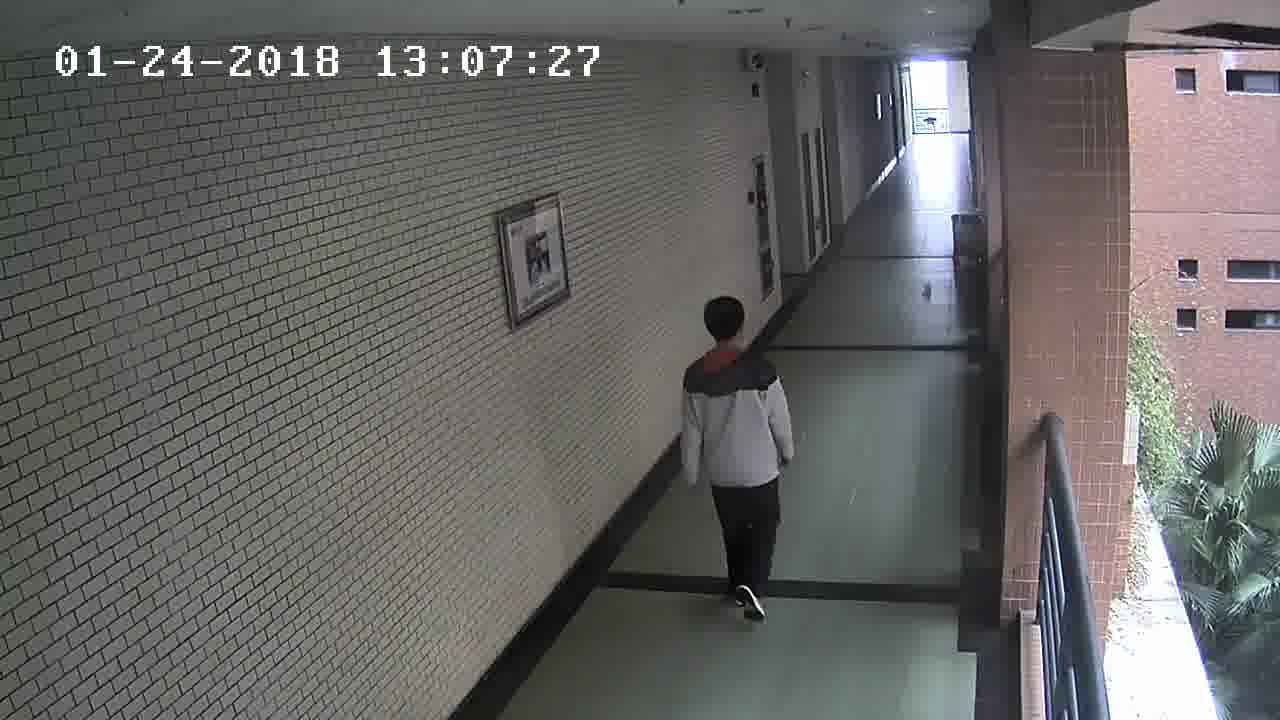
\includegraphics[width=0.3\textwidth]{3-6}
    \caption{最优部署方案}
    \label{fig:rlresult}
\end{figure}

\section{分布式CPU训练}

天河二号拥有约 17920 个计算节点,每个通用节点配备两颗 Xeon E5 系列 12 核心的中央处理器、三个 XeonPhi 57 核心的协处理器(运算加速卡),总内存容量约 1.4PB,全局存储总容量约 12.4PB\cite{tianhe2018config}。2017 年 9 月,天河二号启动升级工程,二期系统天河二号 A 采用国产加速器 Matrix 2000,替换原有的 Xeon Phi 57 加速器,升级后系统峰值运算速度将达到 94.97Pflops\cite{tianhe2017summary}。天河二号各分区的详细配置如表 \ref{tab:tianheconfig}。天河二号的节点分别属于三个分区:CPU 分区、GPU 分区和胖节点分区。本项目使用了天河二号的 GPU 分区,与其它分区最大的不同在于 GPU 分区每个节点都配备了 2 块 NVIDIA Tesla K80 显示卡,显示内存 VRAM 为 24GB,单精度浮点数运算速度为 8.74 TFLOPS,双精度浮点数的运算速度为 2.91 TFLOPS。每个节点同时具备高性能的 CPU 和 GPU 运算能力,方便进行深度神经网络模型训练的对比测试。与此同时,各节点之间通过千兆网络进行连接,可用于搭建多节点分布式计算网络。

天河二号的节点分为登陆节点和计算节点。登陆节点主要用于代码编译、数据解压、环境配置等工作。计算节点配备了高性能的 CPU 和 GPU,主要用于大数据计算,以及大规模的编译任务。登陆节点和计算节点的操作系统均为 CentOS 7,系统使用 slurm 作业管理系统管理作业队列,使用 module 管理各种可选的软件包、运行库。

\begin{table}[!ht]
\centering
\caption{天河二号各分区配置表}
\label{tab:tianheconfig}
\begin{tabularx}{\textwidth}{p{0.08\textwidth}<{\centering}p{0.08\textwidth}<{\centering}p{0.35\textwidth}<{\centering}p{0.10\textwidth}<{\centering}p{0.25\textwidth}<{\centering}}
\toprule
\multicolumn{2}{c}{节点 / 分区}  & CPU                          & 内存    & GPU                  \\ \midrule
\multicolumn{2}{c}{CPU 分区}  & 2 $\times$ 12 Intel Xeon E5-2692 v2 & 64GB  & -                    \\
\multicolumn{2}{c}{GPU 分区}  & 2 $\times$ 10 Intel Xeon E5-2660 v3 & 256GB & 2 $\times$ NVIDIA Tesla K80 \\
\multirow{3}{*}{胖节点} & 128GB & 2 $\times$ 12 Intel Xeon E5-2692 v2 & 128GB & -                    \\
                        & 3TB   & 4 $\times$ 14 Intel Xeon E7-4850 v3 & 3TB   & -                    \\
                        & 6TB   & 8 $\times$ 16 Intel Xeon E7-8867 v3 & 6TB   & -                    \\ \bottomrule
\end{tabularx}
\end{table}

\subsection{多CPU集群分布式训练与单机的比较}

表\ref{tab:comp1}展示了深度行人重识别模型分别在单机及多CPU集群上训练的时间性能。第二行代表模型完整训练一个数据批次(epoch)所需的时间。从表中可以看出,采用多CPU集群取得的时间收益,与CPU节点个数近似地成线性比例关系,仅仅增加了一些节点之间通信的开销。同时,随着节点数目的增加,节点之间的通信开销也没有快速增长的趋势,说明了分布式训练的正确性和有效性。

\begin{table}[!ht]
    \centering
    \caption{多CPU集群分布式训练与单机的比较}
    \label{tab:comp1}
    \begin{threeparttable}
    \begin{tabularx}{\textwidth}{X<{\centering}X<{\centering}X<{\centering}}
    \toprule
    集群节点个数 & 时间~(~s/epoch~) & 分布式开销~(~s~)~\tnote{a} \\ \midrule
    1 & 5821 & 0   \\
    2 & 3016 & 211 \\
    4 & 1536 & 323 \\
    5 & 1219 & 274 \\ \bottomrule
    \end{tabularx}
    \begin{tablenotes}
        \footnotesize
        \item[a] 分布式开销$=$分布式训练所用时间$\times$节点个数$-$单机训练时间
    \end{tablenotes}
    \end{threeparttable}
\end{table}

\subsection{多CPU集群分布式训练与GPU的比较}

本文还将多CPU集群与单机GPU训练深度行人重识别模型进行比较,不出意外的是,单机GPU以326 s/epoch的速度将单机CPU远远甩开,按照表\ref{tab:comp1}的结果估计,大约需要包含20个节点的CPU集群才能追平GPU的速度。由此可见在运算速度上,多CPU集群不占优势。而多CPU集群相对于GPU的优势在于,其可能很轻松地拥有海量的内存,且十分容易扩展,因此可以实现同时大批量数据的运算,增大训练中的 Batch Size,使得模型参数的梯度计算更加准确,从而可以使用更大的学习率。与此同时,根据Smith等人\cite{smith2017don}的研究,在训练过程中动态地增加Batch Size,可以代替动态地衰减学习率。使用大的学习率,可以加速模型参数的收敛,因此训练模型可以经历更少的Epoch,达到加速训练的目的。

% 表\ref{tab:comp2}是多CPU集群(包含5个CPU节点)与GPU在训练深度行人重识别模型时,不同的Batch Size、学习率、Epoch数以及准确率的比较。

% \begin{table}[h!]
%     \centering
%     \caption{多CPU集群分布式训练与GPU的比较}
%     \label{tab:comp2}
%     \begin{threeparttable}
%     \begin{tabularx}{\textwidth}{X<{\centering}X<{\centering}X<{\centering}X<{\centering}X<{\centering}X<{\centering}}
%     \toprule
%     模型    & Batch Size & 学习率~\tnote{a} & Epoch数 & 训练时间~(s) & Rank1~(\%)  \\ \midrule
%     GPU     & 48 & 0.1 & 60 & - & 89.43 \\
%     CPU集群1 & 128 & 0.5 & 40 & - & - \\
%     CPU集群2 & 256 & 1.0 & 30 & - & - \\
%     CPU集群3 & 512 & 2.0 & 20 & - & - \\
%     CPU集群4 & 768 & 3.0 & 10 & - & - \\ \bottomrule
%     \end{tabularx}
%     \begin{tablenotes}
%         \footnotesize
%         \item[a] 初始的基准学习率
%     \end{tablenotes}
%     \end{threeparttable}
% \end{table}
        % 结论与展望
        % conclusion.tex
%
% Aetf <aetf@unlimitedcodeworks.xyz>
% Copyright 2016 Aetf <aetf@unlimitedcodeworks.xyz>
%
% multiple1902 <multiple1902@gmail.com>
% Copyright 2011~2012, multiple1902 (Weisi Dai)
%
% Project Home: https://github.com/Aetf/xjtuthesis
%
% It is strongly recommended that you read documentations located at
%   https://github.com/Aetf/xjtuthesis/wiki
% in advance of your compilation if you have not read them before.
%
% This work may be distributed and/or modified under the
% conditions of the LaTeX Project Public License, either version 1.3
% of this license or (at your option) any later version.
% The latest version of this license is in
%   http://www.latex-project.org/lppl.txt
% and version 1.3 or later is part of all distributions of LaTeX
% version 2005/12/01 or later.
%
% This work has the LPPL maintenance status `maintained'.
%
% The Current Maintainer of this work is Aetf.
%
\chapter{结论与展望}
\echapter{Conclusions}
\cite{niubi-paper}
    \xjtuendcontent

    % 致谢
    % acknowledgements.tex
%
% Aetf <aetf@unlimitedcodeworks.xyz>
% Copyright 2016 Aetf <aetf@unlimitedcodeworks.xyz>
%
% multiple1902 <multiple1902@gmail.com>
% Copyright 2011~2012, multiple1902 (Weisi Dai)
%
% Project Home: https://github.com/Aetf/xjtuthesis
%
% It is strongly recommended that you read documentations located at
%   https://github.com/Aetf/xjtuthesis/wiki
% in advance of your compilation if you have not read them before.
%
% This work may be distributed and/or modified under the
% conditions of the LaTeX Project Public License, either version 1.3
% of this license or (at your option) any later version.
% The latest version of this license is in
%   http://www.latex-project.org/lppl.txt
% and version 1.3 or later is part of all distributions of LaTeX
% version 2005/12/01 or later.
%
% This work has the LPPL maintenance status `maintained'.
%
% The Current Maintainer of this work is Aetf.
%

\xjtuspchapter{致谢}{致\qquad 谢}

\iffalse
感谢国家
\fi


    % 参考文献
    \xjtubib{bibliography}

    % 附录
    \xjtuappendix
        \xjtuappendixchapter{外文文献翻译}

    \begin{center}
        \sihao\textbf{Mask R-CNN:用于预测遮罩的区域卷积神经网络}
    \end{center}

    \textbf{摘要}:我们展现了一个概念意义上简单、稳定以及通用的目标实例划分框架。我们的方法能够高效地检测图片中目标,与此同时还能为目标实例生成高质量的划分遮罩。我们的方法在Faster R-CNN的基础上,增加了一条用于预测目标物体遮罩的分支,与现存的预测目标物体边界框的分支\emph{并行}。我们将此方法称为Mask R-CNN。Mask R-CNN训练简单,且仅比处理帧速为5fps的Faster R-CNN增加了少量的运算量。不仅如此,在Mask R-CNN框架上增加其它的任务也十分简单,例如允许我们在相同的框架下估计人物的姿势。我们的方法在COCO系列挑战中的三个任务都取得了最佳成绩,包括实例分割、边界框目标检测以及人物姿势检测。在没有使用调参技巧的情况下,Mask R-CNN超过了每个任务中所有现存的单一模型框架,包括COCO 2016挑战的冠军。我们希望我们的模型能够成为一个坚实的基础模型,为今后实例级别的识别研究减轻负担。本框架的源代码已经公开在:\url{https://github.com/facebookresearch/Detectron}.

    \xjtuappendixsection{引言}
    在过去很短的时间内,计算机视觉社区快速地提高了目标检测和语义分割的结果。在很大的程度上,一些强大的基础模型驱动了这些结果,例如用于目标检测任务的Fast/Faster R-CNN 框架以及用于语义分割的全卷积网络(FCN)框架。这些方法的概念很新颖,在提供了灵活性和稳健性的同时,也提供了快速的训练和检测。我们本次工作的目标是开发一个同等有效的\emph{实例分割}框架。

    实例分割非常具有挑战性,因为它需要在正确地检测出一张图片中所有目标的同时,精确地划分每一个实例物体。因此实例分割问题包含了传统计算机视觉领域中的\emph{目标检测}和\emph{语义分割}任务。其中目标检测的任务是对于图片中的每一个目标进行分类,并使用边界框定位目标。而语义分割的目标是将图片中的每一个像素分类为一些固定的类别,而不区分每一个目标实例。\footnote{我们使用术语\emph{目标检测}表示检测目标的边界框,而不是遮罩;使用术语\emph{语义分割}表示将每一个像素分类而不区分目标实例,与通用的术语一致。同时我们使用术语\emph{实例分割}来表示既包含语义分割也包含目标检测的任务。} 对于实例分割任务,有人可能会认为需要一个复杂的方法才能得到好的结果。然而我们展示了一个极其简单、灵活以及快速的系统,能够超越先前在实例分割领域最先进的成果。

    我们这个称为\emph{Mask R-CNN}的方法是Faster R-CNN的扩展,增加了一个用于预测每一个感兴趣区域(Region of Interest,RoI)的分割遮罩的分支,该分支与现有的用于分类及边界框回归的分支\emph{并行}(图~\ref{fig:teaser})。该遮罩分支是一个应用于每一个感兴趣区域的全连接卷积网络,用于像素到像素级别的分割遮罩预测。Faster R-CNN框架便于用很多种灵活的架构设计实现,对于一个特定的Faster R-CNN网络,基于此的Mask R-CNN模型很也容易实现和训练。不仅如此,遮罩分支仅增加了少量的计算量,使得一个快速的系统和实验成为可能。

    Mask R-CNN的原则是作为Faster R-CNN的一个直观的扩展框架,然而正确地构造遮罩分支是取得好结果的关键。更重要的是,Faster R-CNN不是为在输入和输出之间像素到像素对齐而设计的。这种设计在\emph{RoIPool}运用粗粒度的空间量化进行特征提取时最为明显。其中RoIPool是\emph{事实上的}处理实例的核心操作。为了解决不对齐的问题,我们提出了简单、免量化的层,称为\emph{RoIAlign},其完整地保留了额外的空间位置。尽管这看上去是一个很小的改变,然而具有很大的影响:它将遮罩预测的准确率相对提升了10\%到50\%,并且在更严格的评估方式下提升更明显。我们的第二个发现是,有必要将遮罩预测与分类预测\emph{解耦}:我们独立地对每个类别进行二元遮罩预测,取消了不同类别之间的竞争,同时利用网络中RoI分类分支进行类别预测。与之相反的,全卷积网络通常用于对每个像素进行多分类操作,该操作将分割与分类耦合起来,这样的传统方法在我们的实验的实例分割任务中表现不佳。

    在没有使用任何调参技巧的情况下,Mask R-CNN的表现超过了所有先前在COCO实例分割任务中最优秀的单模型的结果,包括依靠高度工程化技巧赢得2016年挑战的冠军。作为一个附带的结果,我们的方法在COCO目标检测任务中依然表现出色。在控制变量分析对比实验中,我们评估了模型中多个基本的组成部分,这让我们能够评估模型的稳健性以及分析核心元素的影响。

    我们的模型在单张GPU上每一帧的运行时间大约为200毫秒,在一台拥有8张GPU的机器上使用COCO数据集进行训练大约需要花费两天。我们相信如此快的训练和测试速度,以及模型的灵活性和准确性,能够让今后的实例分割研究获益。

    最后,我们通过利用COCO姿势关键点数据库完成人类姿势估计任务简单展示了该框架的通用性。通过将每一个关键点看作是一个有固定个数1的二元遮罩,再加上一些很小的修改,就可以将原始的Mask R-CNN框架应用于检测每一个人物实例的姿势。在没有任何调参技巧的情况下,Mask R-CNN的表现超过了COCO 2016人物姿势关键点挑战的获胜者,同时检测速度依然是每秒5帧。因此Mask R-CNN可以更宽泛地看作是一个用于\emph{实例级别}的识别的灵活框架,并且可以很轻易地扩展到其它的复杂任务当中。

    我们已经将源代码公开以促进今后的研究工作。

    \xjtuappendixsection{相关工作}

    \paragraph{R-CNN:} 基于区域的卷积神经网络(Region-based CNN,R-CNN)这样的用于边界框目标检测的方法,通常被用于处理大量的目标候选区域,同时独立地在每一个RoI上评估卷积网络。在2014年,经过扩展的R-CNN可通过RoIPool用于处理在特征图上的RoI,使其取得更高的准确率和更快的速度。Faster R-CNN再度扩展了此项工作,其使用区域候选网络(Region Proposal Network,RPN)来学习注意力机制。Faster R-CNN相比于之后的改进模型更加灵活和稳健 ,同时其依然是当前多个评估标准中领先的框架。

    \xjtuendappendix

\end{document}